%*********************PRACA MAGISTERSKA*******************************

\documentclass[12pt, a4paper, oneside, titlepage, final]{book}

%=====================PREAMBUŁA===============================

%**************************************************************************
%**************************************************************************
%**************************PREAMBUŁA***************************************
%**************************************************************************
%**************************************************************************

%***************************PAKIETY****************************************
\usepackage[digitsep]{siunitx}
\usepackage{tocloft}
\usepackage[table,dvipsnames]{xcolor}
\usepackage{StronaTytulowa//strtyt} %mój pakiet ze stroną tytulową
\usepackage{geometry}				%pakiet potrzebny do marginesów
\usepackage{underscore}			%pakiet do właściwej obsługi 
\usepackage{pdflscape}				% horyzontalny układ strony
\usepackage{array}			% pakiet potrzebny do tabel
\newcolumntype{P}[1]{>{\centering\arraybackslash}p{#1}}
\newcolumntype{M}[1]{>{\centering\arraybackslash}m{#1}}
\usepackage[polish]{babel}			%pakiet językowy
\usepackage[pdfencoding=auto]{hyperref}               % pakiet do hiperlinków, pdfencoding potrzebne, że dobrze wyświetlał znaki w zakładkach pdfa
\usepackage[all]{hypcap} 			%pakiet poprawiający działanie hiperlinków
\usepackage{titlesec}				% pakiet do  hiperlinków sekcji
\usepackage{pifont}
\usepackage{moresize}				% dodaje dwie nowe wielkości czcionki ssmall i HUGE
\usepackage{stata//stata}			%pakiet potrzeny do formatu staty
\usepackage{underscore}			%pakiet do właściwej obsługi 
\usepackage{dcolumn}				% pakiet do tabeli ze staty
\usepackage{changepage}
\usepackage{booktabs,tabularx}		% pakiet do tabeli ze staty
\usepackage{graphicx}			% pakiet do grafik
\usepackage{epstopdf}
\usepackage{caption}			% tytuły nad obrazkami
\usepackage{subcaption}
\captionsetup[table]{name=Tabela} %zmiana nazwy z Tabel na Tabela
\captionsetup[figure]{name=Wykres} %zmiana nazwy z Figure na Wykres
\usepackage{floatrow}			% tytuły nad obrazkami
\usepackage{amsmath}			% równania wieloliniowe
\usepackage[OT4]{polski}
\usepackage[utf8]{inputenc} 
\usepackage[T1]{fontenc}
\usepackage{mathptmx}			% Kind of Times New Roman 
\usepackage{cite}				% For citations
\usepackage{url}				% for breaking url
\usepackage{indentfirst}		% pakiet do wcięć na początku rozdziału
\usepackage[hang]{footmisc} 	% pakiet do obsługi layout footnota 1/2
\usepackage{lipsum}				% pakiet do obsługi layout footnota 2/2
\usepackage{amsfonts} % for the \checkmark command 
\usepackage[doublespacing]{setspace} %interlinia w stópce
\usepackage{longtable}		% tabele na kilka stron
\usepackage{multirow}
\usepackage{blindtext}
\usepackage{titlesec}
\usepackage[printonlyused]{acronym}
%**************************************************************************

%*************************USTAWIENIA GLOBALNE*************************
\setcounter{secnumdepth}{0}			%ustawienia hiperlinków
\hypersetup{colorlinks, citecolor=black, filecolor=black, linkcolor=black, urlcolor=black} %kolor hiperlinków
\linespread{1.5} %1.5 odstęp pomiędzy wierszami
\newgeometry{tmargin=2.5cm, bmargin=2.5cm, lmargin=2.5cm, rmargin=2.5cm}
\setlength\footnotemargin{10pt} % ustawianie marginu dla footnota
\pagestyle{plain} %brak nagłówków w całym dokumencie
\floatsetup[figure]{capposition=top}% opisy obrazków na górze rysunku
\floatsetup[table]{capposition=top} % opisy tabel na górze
\captionsetup{labelfont=bf}
%**************************************************************************
\graphicspath{{./Rysunki/}} % ustawia sciezke do rysunków 
\setlength\parindent{1cm} % ustawia rozmiar wcięcia
\setlength\heavyrulewidth{0.05cm} %szerokość toprule w tabelach
\urlstyle{same} % ustawiania tego samego fontu w url co w pliku
\def\sym#1{\ifmmode^{#1}\else\(^{#1}\)\fi} % ustawianie gwiazdek istotności na wydrukach ze staty
\sisetup{output-decimal-marker = {,}}
\addto\captionspolish{\renewcommand{\listfigurename}{Spis wykresów}}
\addto\captionspolish{\renewcommand{\listtablename}{Spis tabel}}

\InputIfFileExists{\jobname.acr}{\def\haveACRO{0}}   
\immediate\openout15=\jobname.acr\relax
\let\oldac=\ac  
\def\ac{%
   \immediate\write15{\string\gdef\string\haveACRO{1}}\oldac} %
\AtEndDocument{\closeout15}
\renewcommand{\cftlottitlefont}{\Large\bfseries}
\renewcommand{\cftloftitlefont}{\Large\bfseries}

%=============================================================

\begin{document}
%=====================STRONA TYTUŁOWA=========================

\uniwersytet{Uniwersytet Warszawski}
\wydzial{Wydział Nauk Ekonomicznych}
\title{Skuteczność niekonwencjonalnej polityki monetarnej Rezerwy Federalnej w~czasie kryzysu gospodarczego}
\podtytul{Analiza dla lat 2008-2016} 
\author{Mateusz Gomulski}
\indeks{293646}
\kierunek{Informatyka i Ekonometria}
\promotor{prof. UW Ryszarda Kokoszczyńskiego}
\katedra{z Zakładu Finansów Ilościowych WNE UW}
\date{Warszawa, styczeń 2017}
\maketitle %tworzy stronę tytułową

%=============================================================

%=====================OŚWIADCZENIE============================

%*********************************Oświadczenie****************************************

\newpage

\vspace{3cm}

{\setlength{\parindent}{0cm}

\textit{Oświadczenie kierującego pracą}

\vspace{0.5cm}

Oświadczam, że niniejsza praca została przygotowana pod moim kierunkiem i stwierdzam, że spełnia ona warunki do przedstawienia jej w postępowaniu o nadanie tytułu zawodowego.
 
\vspace{1.5cm}

\hspace{1cm} Data  \hspace{8cm}  Podpis kierującego pracą

\vspace{8cm}

\textit{Oświadczenie autora pracy}

\vspace{0.5cm}

Świadom odpowiedzialności prawnej oświadczam, że niniejsza praca magisterska została napisana przeze mnie samodzielnie i nie zawiera treści uzyskanych w sposób niezgodny z obowiązującymi przepisami.

\vspace{0.5cm}

Oświadczam również, że przedstawiona praca nie była wcześniej przedmiotem procedur związanych z uzyskaniem tytułu zawodowego w wyższej uczelni.

\vspace{0.5cm}

Oświadczam ponadto, że niniejsza wersja pracy jest identyczna z załączoną wersją elektroniczną.

\vspace{1.5cm}

 \hspace{1cm} Data  \hspace{8cm}  Podpis autora pracy
 
 }

%=============================================================

%=====================STRESZCZENIE============================

%*********************************Streszczenie itp****************************************

\newpage

\vspace{1cm}
\section*{Streszczenie}

\noindent Niniejsza Praca podejmuje problematykę skuteczności niekonwencjonalnej polityki monetarnej stosowanej przez Rezerwę Federalną w~latach 2008-2016, w~szczególności siły jej oddziaływania na amerykańską gospodarkę oraz rynki finansowe. W~kolejnych częściach opisywane są podstawy teoretyczne niekonwencjonalnej polityki monetarnej, literatura badawcza dotycząca problematyki oraz badanie statystyczne mające na celu zweryfikowanie najważniejszych hipotez. Głównym narzędziem badawczym jest model VAR oszacowany na danych miesięcznych pochodzących z~amerykańskiej gospodarki dla lat 2008-2016. Najważniejsze wnioskami są: stwierdzenie istotnego wpływu niekonwencjonalnej polityki monetarnej na wzrost indeksów na giełdach w~USA oraz na wzrost rentowności amerykańskich obligacji skarbowych.

\vspace{1cm}
\section*{Słowa kluczowe}

\noindent niekonwencjonalna polityka monetarna, kryzys gospodarczy, luzowanie pieniężne, Rezerwa Federalna

\vspace{1cm}
\section*{Dziedzina pracy (kody wg programu Socrates-Erasmus)}

\noindent Ekonomia (14300)

\vspace{1cm}
\section*{Tytuł pracy w języku angielskim}

\noindent The effectiveness of unconventional monetary policy of the Federal Reserve during the economic crisis. Analysis for the period of 2008-2016.


%=============================================================

%======================SPIS TREŚCI============================
\newpage
\tableofcontents
%=============================================================

%=========================Główna część========================

% Wstęp
%*********************************WSTĘP****************************************
\newpage
\chapter*{Wstęp}
 \addcontentsline{toc}{chapter}{Wstęp}
 
Wybuch kryzysu gospodarczego w~2008~roku zaburzył równowagę gospodarczą większości krajów współczesnego świata stawiając im nowe wyzwania w~zakresie zarówno polityki fiskalnej, jak i~monetarnej. Szczególnie mocno naruszył on fundamenty gospodarcze takich krajów rozwiniętych jak: Japonia, Stany Zjednoczone, Wielka Brytania, czy strefa euro. Władze monetarne tych krajów po wykorzystaniu większości konwencjonalnych narzędzi polityki pieniężnej zdecydowały się na zastosowanie nadzwyczajnych działań, które miały na celu pobudzenie wzrostu gospodarczego poprzez stymulowanie akcji kredytowej banków komercyjnych. Zespół tych nadzwyczajnych działań władz monetarnych został następnie określony mianem niekonwencjonalnej polityki monetarnej (ang. \textit{Unconventional Monetary Policy - UMP})\footnote{W dalszej części pracy określana skrótem \acs{NPM}} po to by zaznaczyć ich odrębność w~stosunku do konwencjonalny metod działań banków centralnych. Poniższa praca powstała w~celu zgłębienia tematyki niekonwencjonalnej polityki monetarnej, starając się zarysować jej podstawy teoretyczne oraz sprawdzić jej skuteczność w~kontekście oddziaływania na gospodarkę oraz rynki finansowe.

W niniejszej pracy autor jako hipotezę badawczą przyjął, iż \textbf{niekonwencjonalna polityka monetarna Rezerwy Federalnej stosowana od 2008~roku zamiast pobudzać do wzrostu realnego \acs{PKB} oraz~zbliżać amerykańską gospodarkę do pełnego zatrudnienia przyczyniła się przede wszystkim do wygenerowania ponadprzeciętnych wzrostów cen akcji notowanych na giełdach w~Stanach Zjednoczonych}. Kolejne rozdziały niniejszej pracy maję na celu zebranie informacji koniecznych do zweryfikowania tej hipotezy.

Pierwszy rozdział poświęcony został zarysowaniu podstaw teoretycznych niekonwencjonalnej polityki monetarnej, w~tym w~szczególności zdefiniowaniu i~usystematyzowaniu najważniejszych jej instrumentów oraz kanałów jej transmisji do realnej gospodarki. Wydaje się to niezbędne by móc bez wątpliwości przystąpić do weryfikacji hipotezy badawczej. Drugi rozdział stanowi przegląd wybranych artykułów badawczych poruszających zagadnienie \acs{NPM} w~kontekście jej zastosowania w~przez Rezerwę Federalnej w~latach 2008-2016. Analiza przeprowadzona w~tym rozdziale pozwoli przeanalizować hipotezy badawcze zawarte w~innych pracach badawczych oraz sposoby ich weryfikacji. Ostatni rozdział początkowo koncentruje się na opracowaniu odpowiednich modeli statystycznych, które posłużą do weryfikacji hipotezy badawczej, następnie dochodzi do ich oszacowania, przedstawienia wyników, wyciągnięcia finalnych wniosków  oraz weryfikacji hipotez.

Jako główne narzędzie badawcze w~niniejszej pracy posłuży model wektorowej autoregresji (ang. \textit{Vector Autoregressive Model - VAR}), który został wybrany ze względu na dużą częstość stosowania w~literaturze badawczej poruszającej zagadnienie niekonwencjonalnej polityki monetarnej. Badanie zostanie przeprowadzone dla lat 2008-2016, na danych miesięcznych z~amerykańskiej gospodarki, w~ogromnej większości pochodzących ze strony internetowej Banku Rezerwy Federalnej Saint Louis (\url{http://research.stlouisfed.org}). Wyniki uzyskane z~modelu \acs{VAR} zostaną przeanalizowane za pomocą: funkcji odpowiedzi na impuls, dekompozycji wariancji błędów prognoz oraz analizy wstecznej trafności prognoz uzyskanych z~modelu.
% Podstawy Teoretyczne Modelu
\newpage
\chapter*{Rozdział 1 \\ \vspace{1cm} \Large{Podstawy teoretyczne niekonwencjonalnej polityki monetarnej}}
\addcontentsline{toc}{chapter}{1. Podstawy teoretyczne niekonwencjonalnej polityki monetarnej}

\noindent Pierwszy rozdział niniejszej pracy został poświęcony przeglądowi i~usystematyzowania dostępnej wiedzy dotyczącej niekonwencjonalnej polityki monetarnej (ang. \textit{Unconventional Monetary Policy - UMP}),  a~w~szczególności jej najważniejszych narzędzi oraz kanałów transmisji do realnej gospodarki. Jasne i~przejrzyste zdefiniowanie pojęć związanych z~niekonwencjonalną polityką monetarną jest o~tyle istotne, iż polityka ta jest zagadnieniem stosunkowo nowym - do czasu wybuchu światowego kryzysu gospodarczego w~2008 roku była ona rzadko opisywana w~literaturze badawczej. Omawiany rozdział został podzielony na trzy części. Pierwsza z~nich skupia się na wstępnym, ogólnym nakreśleniu pojęcia niekonwencjonalnej polityki pieniężnej. Druga część rozdziału została poświęcona szczegółowemu opisowi i~klasyfikacji instrumentów niekonwencjonalnej polityki pieniężnej wraz z~przedstawieniem przykładów ich zastosowania przez władze monetarne kilku krajów świata. Ostatnia części niniejszego rozdziału prezentuje potencjalne kanały transmisji impulsów monetarnych niekonwencjonalnej polityki pieniężnej do realnej gospodarki. Celem omawianego rozdziału będzie więc zapoznanie czytelnika z~najważniejszymi podstawami teoretycznymi  niekonwencjonalnej polityki monetarnej, tak aby mógł on w~pełni zrozumieć sens oraz specyfikę problemu badawczego poruszanego w~niniejszej pracy. Zrozumienie tych kwestii będzie kluczowe do właściwej analizy treści zamieszczonych w~kolejnych rozdziałach oraz interpretacji wniosków wypływających z~całości przeprowadzonego badania.

\phantomsection	
\hypertarget{podroz11}{}
\section*{\large{1.1. Najważniejsze założenia niekonwencjonalnej polityki monetarnej}}
\addcontentsline{toc}{section}{1.1. Najważniejsze założenia niekonwencjonalnej polityki monetarnej}

Terminem niekonwencjonalna polityka monetarna w~literaturze badawczej określa się zazwyczaj zbiór ponadstandardowych działań banków centralnych w~takich krajach jak Stany Zjednoczone, Wielka Brytania, Japonia, Szwajcaria czy kraje strefy euro w~reakcji na wybuch światowego kryzysu gospodarczego w~2008 roku. Niekonwencjonalność tych działań nie wynika jednak z~faktu, iż zostały one pierwszy raz zastosowane po wybuchu ostatniego kryzysu gospodarczego, gdyż większość z~nich była już wcześniej stosowana przez władze monetarne różnych krajów świata na przestrzeni ostatnich 100~lat (w~zmodyfikowanych wariantach). Niekonwencjonalne w~tym przypadku są skala i~intensywność ich stosowania, zakres oddziaływania na rynki finansowe oraz wpływ na wielkość i~kompozycję bilansu banku centralnego oraz bilansów uczestników rynków finansowych zarówno z~sektora prywatnego, jak i~publicznego. Niekonwencjonalne działania banków centralnych ze statusu ciekawostek orientalnej lub prehistorycznej bankowości centralnej zyskały status głównych instrumentów do walki z~największym kryzysem finansowym od czasu wielkiego kryzysu gospodarczego lat 30.~XX~wieku. Stąd też wzbudzają one ogromne zainteresowanie współczesnych ekonomistów oraz przedostały się do świadomości społecznej szerokiej rzeszy ludności na całym świecie. Brak jest jednak jednoznacznej klasyfikacji i~terminologii dotyczącej niekonwencjonalnej polityki monetarnej - w~wielu pracach badawczych pojawiają się często sprzeczne jej definicje, co utrudnia prowadzenie efektywnej debaty na temat jej pożyteczności, czy też skuteczności. Dlatego też w~tej części rozdziału przedstawiona zostanie jasna klasyfikacja i~terminologia dotycząca badanych niekonwencjonalnej polityki pieniężnej tak, aby maksymalnie ułatwić czytelnikowi zrozumienie istoty badanego w~niniejszej pracy problemu unikając mylących uproszczeń i~generalizacji.

\textbf{Niekonwencjonalna polityka monetarna to zespół nadzwyczajnych działań władz monetarnych oddziałujących na gospodarkę danego kraju za pomocą zmian w~wartości lub kompozycji bilansu banku centralnego. Działania te są najczęściej podejmowane w~sytuacji głębokiego kryzysu gospodarczego lub w~jego następstwie, gdy konwencjonalne narzędzia polityki monetarnej nie przynoszą oczekiwanych efektów. Ich głównym celem jest wywarcie presji na obniżenie stóp procentowych na rynku międzybankowym w~momentach wzmożonej niepewności pomiędzy uczestnikami tego rynku - nadmiernej premii za ryzyko}. Cel ten jest realizowany poprzez obniżanie średnio- i~długoterminowych rynkowych stóp procentowych za pomocą zakupów przez władze monetarne dłużnych papierów wartościowych o~znacznej wartości od banków komercyjnych oraz inwestorów instytucjonalnych. Bezpośrednim skutkiem większości takich operacji jest wzrost bazy monetarnej. Niekonwencjonalna polityka pieniężna jest polityką czysto bilansową oznacza to, iż poprzez zmiany w~kompozycji (strukturze udziału poszczególnych aktywów/pasywów lub średniej zapadalności portfela) i~w~wartości bilansu banku centralnego władze monetarne starają się wpłynąć na kompozycję i~wielkość bilansów członków sektora publicznego i~prywatnego. To w~jaki sposób dany niekonwencjonalny instrument oddziałuje na bilans banku centralnego jest najczęściej spotykanym wyznacznikiem ich podziału.

\phantomsection % do hiperlinków dla sekcji w spisie treści
\hypertarget{podroz11}{}
\section*{\large{1.2. Podstawowe instrumenty niekonwencjonalnej polityki monetarnej}}
\addcontentsline{toc}{section}{1.2. Podstawowe instrumenty niekonwencjonalnej polityki monetarnej}

Podstawowe instrumenty niekonwencjonalnej polityki monetarnej można podzielić na dwie grupy ze względu na sposób oddziaływania na bilans banku centralnego: instrumenty powodujące zmianę wartości bilansu banku centralnego oraz instrumenty niepowodujące takiej zmiany - zmieniające jedynie udział/strukturę poszczególnych aktywów w~bilansie lub średni czas zapadalności jego składników.

\phantomsection % do hiperlinków dla sekcji w spisie treści
\hypertarget{podroz111}{}
\subsection*{\large{1.2.1. Instrumenty powodujące zmianę wartości bilansu banku centralnego}}
\addcontentsline{toc}{subsection}{1.2.1. Instrumenty powodujące zmianę wartości bilansu banku centralnego}

Do grupy niekonwencjonalnych instrumentów polityki pieniężnej powodujących zmianę wartości bilansu banku centralnego należy zaliczyć:

\begin{itemize}
\setlength\itemsep{0.05cm}
\item luzowanie ilościowe (ang. \textit{Quantitative Easing - QE}),
\item luzowanie kredytowe (ang. \textit{Credit Easing - CE}),
\item długoterminowe operacje refinansowe (ang. \textit{Long Term Refinancing Operations - LTRO}),
\item ujemne stopy procentowe (ang. \textit{Negative Interest Rates - NIR}).
\end{itemize}

\textbf{Luzowanie ilościowe} jest niekonwencjonalnym instrumentem polityki pieniężnej stosowanym przez władze monetarne w~formie zakupów od banków komercyjnych długoterminowych krajowych obligacji rządowych lub innych długoterminowych instrumentów finansowych gwarantowanych przez skarb państwa. Transakcje te mają zazwyczaj na celu spłaszczenie krzywej dochodowości dłużnych papierów skarbowych poprzez wpływanie na wzrost ich cen, a~finansowane są ze środków pieniężnych uzyskanych przez powiększenie bilansu banku centralnego prowadzące do wzrostu bazy monetarnej. W~trakcie przeprowadzania tej operacji główny nacisk kładziony jest na monitorowanie wzrostu wartości nadobowiązkowych rezerw trzymanych przez banki komercyjne na kontach w~banku centralnym, bardziej istotne w~tym przypadku są więc pasywa banku centralnego, a~nie skład i~kompozycja jego aktywów. Takie działanie władz monetarnych ma skłonić banki komercyjne do obniżenia kosztów uzyskania kredytów dla gospodarstw domowych i~przedsiębiorstw, zwiększyć krajowy popyt wewnętrzny i~inwestycje, a~w~konsekwencji pobudzić wzrost gospodarczy oraz inflację. Bank Japonii jako pierwszy wprowadził i~zastosował instrument o~nazwie luzowanie ilościowe w~latach 2001-2006, aby zwalczyć deflację i~pobudzić wzrost gospodarczy. W~różnych wariantach i~z~różnymi skutkami instrument ten był wykorzystywany po wybuchu kryzysu finansowego z~2008 roku przez banki centralne Stanów Zjednoczonych, Wielkiej Brytanii, strefy euro oraz Japonii.

Szczególnym przypadkiem zastosowania luzowania ilościowego są działania Szwajcarskiego Banku Narodowego (SBN) na tamtejszym rynku pieniężnym w~sierpniu 2011~roku. Działania te różniły się od klasycznej definicji luzowania ilościowego głównie tym, iż władze monetarne Szwajcarii skupowały od banków komercyjnych przede wszystkim krótkoterminowe papiery wartościowe (bony pieniężne), a~nie długoterminowe obligacje skarbowe - niekonwencjonalna polityka monetarna miała pomóc w~dalszym obniżaniu krótkoterminowych stóp procentowych\footnote{Część badaczy sugeruje, iż pomimo przeprowadzania interwencji jedynie na rynku pieniężnym Szwajcarski Bank Narodowy doprowadził również do obniżenia rentowności długoterminowych obligacji skarbowych poprzez znaczące zwiększenie wartości rezerw nadobowiązkowych\cite{christensen21}}. Wyjątkowa była też skala interwencji w~relatywnie krótkim czasie - w~ciągu trzech tygodni \acs{SBN} wydał na zakup bonów pieniężnych ponad 170~miliardów franków szwajcarskich czyli równowartość 30\% krajowego \acs{PKB}. Żaden bank centralny nie powiększał swojego bilansu w~tamtym czasie w~tak gwałtownym tempie - od 3~sierpnia do 17~sierpnia 2011~roku wartość bilansu Szwajcarskiego Banku Narodowego wzrosła o~ponad 40\% \cite{christensen21}. Bezpośrednim celem tych niekonwencjonalnych działań \acs{SBN} było doprowadzanie do deprecjacji kursu krajowej waluty. Podobnie jak w~przypadku innych zastosowań luzowania ilościowego kładziono główny nacisk na modelowanie wzrostu wartości rezerw nadobowiązkowych banków komercyjnych w~banku centralnym, co miało doprowadzić do silnego osłabienia kursu franka szwajcarskiego (znaczące obniżenie krótkoterminowych krajowych stóp procentowych miało odstraszyć zagranicznych inwestorów), a~w~konsekwencji pobudzić eksport i~zapobiec deflacji.

\textbf{Luzowanie kredytowe} jest niekonwencjonalnym instrumentem polityki pieniężnej stosowanym przez władze monetarne w~formie zakupów od uczestników rynków finansowych nieskarbowych dłużnych papierów wartościowych, przede wszystkim: obligacji przedsiębiorstw, obligacji przedsiębiorstw sponsorowanych przez rząd (ang. \textit{Government-Sponsored Enterprise - GSE}), papierów komercyjnych przedsiębiorstw, listów zastawnych oraz papierów wartościowych opartych na aktywach (ang. \textit{Asset-Backed Securities - ABS}). Celem tej operacji jest zmniejszenie spreadu kredytowego pomiędzy oprocentowaniem obligacji skarbowych, a~oprocentowaniem nieskarbowych papierów dłużnych o~zbliżonym ratingu. Takie działanie ma doprowadzić do obniżenia rentowności kupowanych instrumentów, zachęcić uczestników rynku do dokonywania innych bardziej ryzykownych inwestycji i~w~konsekwencji doprowadzenie do obniżenia kosztów uzyskania kredytu dla gospodarstw domowych i~przedsiębiorstw. Podobnie jak w~przypadku luzowania ilościowego, luzowanie kredytowe prowadzi do wzrostu wartości bilansu banku centralnego, gdyż zakupy nowych nieskarbowych instrumentów dłużnych odbywają się zazwyczaj za pomocą środków pieniężnych specjalnie na ten cel wygenerowanych. 

W~przeciwieństwie do luzowania ilościowego w~luzowaniu kredytowym władze monetarne nie koncentrują się na stronie pasywów bilansu banku centralnego tylko na stronie aktywów - jak ich kompozycja i~średnia zapadalność wpływa na warunki uzyskania kredytu przez gospodarstwa domowe i~przedsiębiorstwa. Luzowanie kredytowe w~sposób oczywisty wpływa na narażenie bilansu banku centralnego na większe ryzyko niż to jest w~przypadku luzowania ilościowego, gdyż nieskarbowe dłużne papiery wartościowe charakteryzują się dużo niższą płynnością i~większym stopniem ryzyka bankructwa niż papiery gwarantowane przez skarb państwa. Dlatego też stosując ten instrument władze monetarne powinny w~sposób bardziej ostrożny i~precyzyjny dobierać kupowane aktywa, tak by nie narazić swojego bilansu na zbyt dużą ekspozycję na ryzyko. Po 2008~roku z~luzowania kredytowego korzystały banki centralne Stanów Zjednoczonych, Wielkiej Brytanii oraz Japonii.

\textbf{Długoterminowe operacje refinansowe} to jedno z~podstawowych narzędzi Europejskiego Banku Centralnego (EBC) stosowane by zarządzać średnioterminową płynnością banków komercyjnych strefy euro poprzez udzielanie pożyczek pieniężnych pod zastaw papierów wartościowych o~określonej jakości. W~swojej podstawowej formie (zapadalność do 6~miesięcy, wysokie wymagania co do zabezpieczenia, ograniczona dostępność środków, nieistotny wpływ na wielkość bilansu banku centralnego), należy zaliczyć to narzędzie do jednej z~lokalnych modyfikacji transakcji depozytowo-kredytowych. Jednak w~grudniu 2011~roku oraz w~lutym 2012~roku długoterminowe operacje refinansowe zostały zawarte z~bankami komercyjnymi strefy euro na zupełnie innych warunkach niż dotychczas sprawiając, iż można je było zacząć zaliczać do niekonwencjonalnych narzędzi polityki pieniężnej. 

Przede wszystkim wydłużono czas na spłatę pożyczki udzielonej przez bank centralny, zazwyczaj omawiane w~poprzednim akapicie transakcje były zawierane na czas jednego miesiąca\cite{ebc22}, w~szczególnych przypadkach było to 6~miesięcy. Jednak transakcje zawierane w~grudniu 2011~i~w~lutym 2012~miały trzyletnią zapadalność po to by zapewnić długookresową wypłacalność zainteresowanym instytucjom. Poza tym rozszerzono paletę możliwych zabezpieczeń pod te transakcje o~papiery wartościowe z~niskim ratingiem oraz wcześniej nie wykorzystywane instrumenty finansowe, po to by banki komercyjne mogły, w~szczególności, pozbyć się ze swoich bilansów obligacji skarbowych krajów strefy euro zagrożonych bankructwem (tzw. kraje \acs{PIIGS}\footnote{Do krajów \acs{PIIGS} zaliczane były następujące europejskie kraje: Portugalia (ang. \textit{\textbf{P}ortugal}), Irlandia (ang. \textit{\textbf{I}reland}), Włochy (ang. \textit{\textbf{I}taly}), Grecja (ang. \textit{\textbf{G}reece}) oraz Hiszpania (ang. \textit{\textbf{S}pain}).}. Dodatkowo każdy bank zainteresowany zawarciem długoterminowej operacji refinansowej mógł pozyskać od EBC dowolną kwotę pieniężną, nie było ograniczeń co do wartości transakcji. W~końcu koszt pozyskania środków w~ramach transakcji z~przełomu 2011~i~2012~roku był niezwykle korzystny. Stąd też długoterminowe operacje refinansowe z~21 grudnia 2011~roku i~29 lutego~2012 roku cieszyły się ogromnym zainteresowaniem skorzystało z~nich ponad 800~banków komercyjnych strefy euro pozyskując łącznie ponad bilion euro. Tak duży popyt na środki pieniężne spowodował proporcjonalny wzrost wartości bilansu Europejskiego Banku Centralnego oraz nieproporcjonalny wzrost ryzyka w~tym bilansie spowodowany głównie przyjmowaniem w~zastaw toksycznych obligacji skarbowych. Zmieniona została więc kompozycja bilansu \acs{EBC} pod kątem udziału poszczególnych aktywów oraz ryzykowności i~średniej zapadalności zarówno aktywów jak i~pasywów. 

W~czerwcu 2014~roku Europejski Bank Centralny ogłosił program będący modyfikacją programu długoterminowych operacji refinansowych nazywając go programem ukierunkowanych długoterminowych operacji refinansowych (ang. \textit{Targeted Long Term Refinancing Operations - TLTRO}). Główną różnicą w~stosunku do poprzedniego programu był fakt, iż wartość środków, które dany bank komercyjny mógł uzyskać od Europejskiego Banku Centralnego w ramach \acs{TLTRO} wynosiła do 7\% wartości pożyczek, które dany bank udzielił gospodarstwom domowym (z~wyłączeniem kredytów hipotecznych) oraz przedsiębiorstwom niefinansowym. Środki pozyskane w~ramach ukierunkowanych długoterminowych operacji refinansowych mogły mieć maksymalnie czteroletnią zapadalność, a~ich oprocentowanie było stałe i~równe głównej stopie refinansowej w~strefie euro w~momencie ich pozyskania powiększonej o~10 punktów bazowych. W~ramach 7~aukcji \acs{TLTRO}, pomiędzy październikiem 2014~a~czerwcem 2016, Europejski Bank Centralny przekazał bankom komercyjnym w~strefie euro około 425~miliardów euro zastępując wygasające na początku 2015~roku operacje \acs{LTRO}. 10~Marca~2016 roku władze monetarne strefy euro ogłosiły kolejny program ukierunkowanych długoterminowych operacji refinansowych (TLTRO2), który różni się w~stosunku do swojego poprzednika przede wszystkim tym, iż wynagradza on banki, które zwiększą wartość udzielonych pożyczek dla przedsiębiorstw niefinansowym i~gospodarstw domowych o~2,5\% w~ciągu dwóch lat \cite{tahiri33}.

\textbf{Ujemne stopy procentowe} dotyczą oprocentowania nadobowiązkowych rezerw oraz krótkoterminowych depozytów banków komercyjnych w~banku centralnym i~do momentu wybuchu kryzysu finansowego w~2008~roku zastosowane zostały tylko raz - w~latach 70. XX wieku przez Szwajcarski Bank Narodowy. Miało to miejsce tuż po upadku systemu walutowego z~Bretton-Woods, w~latach 1972-1978, celem ich zastosowania była obrona kursu franka szwajcarskiego przed zbyt silną aprecjacją, która osłabiała konkurencyjność eksportu Szwajcarii\cite{megg23}. Po 2008~roku narzędzie to w~podobnym celu wykorzystywała również Szwecja (2012), Dania (2012) oraz ponownie Szwajcaria (2014). 

Europejski Bank Centralny ogłosił 5~czerwca~2014~roku wprowadzenie ujemnych stóp procentowych. Intencją władz monetarnych strefy euro było pobudzenie inflacji oraz wzrostu gospodarczego w~unii walutowej. Miało to nastąpić poprzez skłonienie banków komercyjnych głównie z~północy strefy euro do zmniejszania nadobowiązkowych rezerw deponowanych w~\acs{EBC} za pomocą transakcji z~bankami z~południa oraz poprzez spłacanie zawartych na przełomie 2011~i~2012~roku 3-letnich długoterminowych operacji refinansowych, co z~kolei miało wpłynąć na obniżenie kosztów uzyskania kredytu. Ujemne stopy procentowe poprzez koszty odsetek od utrzymywanego w~banku centralnym kapitału mogą wpływać na stopniowe wycofywanie go z~depozytów, co powinno w~dłuższym okresie prowadzić do zmniejszania bilansu banku centralnego i~zmianę jego kompozycji szczególnie po stronie pasywów.

\phantomsection % do hiperlinków dla sekcji w spisie treści
\hypertarget{podroz112}{}
\subsection*{\large{1.2.2. Instrumenty niepowodujące zmiany wartości bilansu banku centralnego}}
\addcontentsline{toc}{subsection}{1.2.2. Instrumenty niepowodujące zmiany wartości bilansu banku centralnego}

Do grupy niekonwencjonalnych instrumentów polityki pieniężnej niepowodujących zmiany wartości bilansu banku centralnego (wpływających jedynie na strukturę poszczególnych aktywów/pasywów lub średnią zapadalność portfela) należy zaliczyć dwa narzędzia wykorzystywane dotąd przez Europejski Bank Centralny (pierwsze z~nich) oraz Rezerwę Federalną (drugie z~nich):

\begin{itemize}
\setlength\itemsep{0.05cm}
\item luzowanie jakościowe (ang. \textit{Qualitative Easing - QLE}),
\item operację Twist (ang. \textit{Operation Twist - OT}).
\end{itemize}

\textbf{Luzowanie jakościowe} jest niekonwencjonalnym instrumentem polityki pieniężnej stosowanym przez władze monetarne w~formie zakupów niskopłynnych aktywów finansowych obarczonych znaczącym ryzykiem przy jednoczesnej sprzedaży wysokopłynnych aktywów obarczonych niższym ryzykiem. Stosowanie tego narzędzia nie powoduje więc zmiany wartości bilansu banku centralnego, gdyż środki pieniężne na nowe zakupy pozyskiwane są ze sprzedaży posiadanych papierów, następuje jednak narastanie ryzyka w~bilansie banku centralnego przeprowadzającego tego rodzaju operacje. Celem przeprowadzania luzowania jakościowego jest najczęściej chęć wpłynięcia na obniżenie rentowności konkretnej grupy dłużnych papierów wartościowych lub przywrócenie odpowiedniej płynności na konkretnym rynku finansowym. Przykładem zastosowania omawianego w~tym akapicie instrumentu są interwencje Europejskiego Banku Centralnego na rynku obligacji skarbowych krajów strefy euro w~latach 2010-2012, kiedy to \acs{EBC} skupował obligacje krajów \acs{PIIGS} (głównie Grecji), w~celu obniżenia rentowności tych papierów, ale również po to aby wykupić toksyczne aktywa z~bilansów instytucji finansowych strefy euro\cite{bagus23}.

\textbf{Operacja Twist\footnote{Operacja Twist nie jest oficjalną nazwą stosowaną przez władze monetarne Stanów Zjednoczonych. W~momencie wprowadzania tego instrumentu w~2011~roku został on nazwany \textit{Maturity Extension Program - MEP}, czyli Program Wydłużenia Zapadalności.}} jest niekonwencjonalnym instrumentem polityki pieniężnej stosowanym przez władze monetarne w~formie sprzedawania przez bank centralny krótkoterminowych obligacji skarbowych (zapadalność do trzech lat) przy jednoczesnym kupowaniu długoterminowych obligacji skarbowych (zapadalność powyżej pięciu lat). W~ten sposób wydłużana jest średnia zapadalność aktywów znajdujących się w~bilansie banku centralnego (bez wpływu na średnią zapadalność pasywów), skróceniu ulega natomiast średnia zapadalność aktywów znajdujących się w~bilansach uczestników rynku finansowego. Głównym celem operacji Twist jest wpłynięcie na spłaszczenie krzywej dochodowości dłużnych papierów rządowych poprzez podniesienie cen długoterminowych obligacji skarbowych i~obniżenie cen ich krótkoterminowych odpowiedników, co podobnie jak w~przypadku luzowania ilościowego i~kredytowego ma wpłynąć na obniżenie kosztów uzyskania kredytów przez gospodarstwa domowe i~przedsiębiorstwa. Najważniejszą zaletą operacji Twist jest brak wpływu na zmianę wartości bilansu banku centralnego oraz umocnienie krajowego kursu walutowego. Największymi ograniczeniami tej operacji są skończony zasób obligacji długoterminowych, które władze monetarne mogą sprzedać w~danym momencie oraz zaburzenie relacji pomiędzy zapadalności aktywów i~pasywów w~bilansie banku centralnego. Operację Twist zastosowano dotychczas dwukrotnie w~Stanach Zjednoczonych w~latach 1961-1965 oraz 2011-2012.

Analiza wniosków wypływających z~zagadnień poruszanych w~niniejszym podrozdziale wskazuje, iż banki centralne posiadają szeroką paletę niekonwencjonalnych instrumentów polityki pieniężnej, dzięki którym są w~stanie reagować na pojawiające się ryzyka w~systemie finansowym. Jednak skuteczność wszelkich działań władz monetarnych szczególnie w~oddziaływaniu na szeroką gospodarkę zależy w~dużej mierze od drożności i~efektywności kanałów transmisji impulsów polityki monetarnej. Dlatego przed przystąpieniem do analizy empirycznej warto rozpoznać i~wyszczególnić najważniejsze kanały transmisji monetarnej, za pomocą których bank centralny może wpływać na badany system finansowy. Temu zagadnieniu poświęcony został kolejny podrozdział.

\phantomsection	% do hiperlinków dla sekcji w spisie treści
\section*{\large{1.3. Kanały transmisji impulsów niekonwencjonalnej polityki monetarnej}}
\addcontentsline{toc}{section}{1.3. Kanały transmisji impulsów niekonwencjonalnej polityki monetarnej}

W~poprzednich dwóch podrozdziałach przedstawiono definicję niekonwencjonalnej polityki monetarnej oraz wskazano główne narzędzia, za pomocą których banki centralne mogą tę politykę realizować. Jednak wspomniane narzędzia nie działają bezpośrednio na system finansowy i~gospodarczy, zazwyczaj służą one jedynie do stymulowania konkretnych procesów, które w~konsekwencji mają wywołać oczekiwany efekt w~realnej gospodarce. Efekt ten jest osiągany zazwyczaj za pomocą tzw. kanałów transmisji polityki monetarnej, czyli ścieżek, dzięki którym impulsy pieniężne wysyłane przez bank centralny docierają do podmiotów gospodarczych takich jak gospodarstwa domowe czy przedsiębiorstwa. Do najważniejszych z~nich w kontekście niekonwencjonalnej polityki monetarnej należą:

\begin{itemize}
\setlength\itemsep{0.05cm}
\item kanał pożyczek bankowych,
\item kanał cen akcji,
\item kanał kursu walutowego,
\item kanał oczekiwań.
\end{itemize}

\noindent Każdy z~wymienionych powyżej kanałów posiada swoją specyfikę - w~odrębny sposób i~z~różnym natężeniem oddziałuje na realną gospodarkę. Dlatego też warto szczegółowo przeanalizować każdy z~nich, aby w~pełni zrozumieć mechanizmy warunkujące ich funkcjonowanie.

\subsubsection*{\normalsize{Kanał pożyczek bankowych}}

Kanał pożyczek bankowych jest związany ze specjalną rolą banków komercyjnych, które zapewniają dostęp do rynku kredytowego podmiotom, które bez pośrednictwa banku nie mogłyby uczestniczyć w~tym rynku ze względu na niski wolumen potrzebnych środków oraz brak szczegółowej informacji o~ich sytuacji finansowej. Władze monetarne mogą starać się stymulować zmiany w~podaży kredytów udzielanych przez banki komercyjne podmiotom prywatnym za pomocą kształtowania wartości rezerw znajdujących się na kontach w~banku centralnym. Robią to w~szczególności stosując niekonwencjonalną politykę monetarną, gdzie wygenerowane nadobowiązkowe rezerwy silnie przewyższają stany w~konwencjonalnych czasach. Im wyższa wartość nadobowiązkowych rezerw tym banki komercyjne mają silniejszą skłonność do udzielania kredytów, aby zaabsorbować w~swoich bilansach dodatkową płynność. Działanie omawianego w~tym paragrafie kanału transmisji monetarnej w kontekście niekonwencjonalnej polityki monetarnej można zobrazować za pomocą poniższego schematu przyczynowo-skutkowych:

\begin{equation}
UMP\uparrow \Longrightarrow R\uparrow \Longrightarrow L\uparrow \Longrightarrow I\uparrow \Longrightarrow Y\uparrow	
\end{equation}
\vspace{-1cm}
\begin{adjustwidth}{2.5em}{0pt}
{\footnotesize Gdzie:  \\
$UMP$ - niekonwencjonalna polityka monetarna, \\
$R$ - rezerwy banków komercyjnych na koncie w~banku centralnym, \\
$L$ - zagregowana wartość udzielonych pożyczek, \\
$I$ - wydatki inwestycyjne (również wydatki konsumpcyjne), \\
$Y$ - zagregowana produkcja.}
\end{adjustwidth}
\vspace{0.3cm}

\noindent Ważną implikacją zaprezentowanego powyżej rozumowania jest fakt, iż niekonwencjonalna polityka pieniężna oddziałująca przez kanał pożyczek bankowych powinna silniej wpływać na wydatki inwestycyjne małych i~średnich firm niż dużych przedsiębiorstw. Dzieje się tak gdyż to właśnie małe i~średnie firmy mają silnie ograniczony dostęp do rynku kredytowego (nie są w~stanie emitować obligacji) i~muszą polegać na kredytach udzielonych im przez banki.

Podstawowym zamysłem władz monetarnych większości krajów świata była naprawa wadliwie działającego po kryzysie kanału pożyczek bankowych za pomocą kilku uzupełniających się mechanizmów. Pierwszym z~nich było przywrócenie płynności na rynku międzybankowym, poprzez większą elastyczność banku centralnego przy zawieraniu operacji repo z~bankami komercyjnymi (m.in. większy wachlarz instrumentów akceptowalnych jako zabezpieczenie, dłuższy okres zawierania transakcji, większa ilość dopuszczonych do operacji podmiotów). Kolejnym etapem naprawy kanału pożyczek bankowych było wygenerowanie na kontach banków komercyjnych w~banku centralnym ogromnych nadmiarowych rezerw poprzez zakup od nich długoterminowych instrumentów dłużnych. Miało to zarówno obniżyć rentowność tych instrumentów (zniechęcając banki do dalszego inwestowania w~nie), jak i~udostępnić bankom środki, które te mogłyby przeznaczyć na udzielanie nowych kredytów. Skuteczność opisanych powyżej działań udrażniających kanał kredytowy jest przedmiotem analizy w~dalszej części niniejszej pracy.

\subsubsection*{\normalsize{Kanał cen akcji}}

Kanał cen akcji można podzielić na dwa mechanizmy: związany z~teorią q~Tobina oraz związany z~efektem majątkowym oddziałującym na konsumpcję. Teoria q~Tobina dostarcza podstaw do analizy w~jaki sposób polityka monetarna może wpływać na gospodarkę poprzez zmiany wycen akcji. Została ona opisana przez Jamesa Tobina w~1969~roku w~artykule \textit{A general equilibrium approach to monetary theory} i~zakładała wyznaczanie współczynnika q~powstałego przez podzielenie wyceny kapitału na giełdzie przez ekonomiczny koszt jego odtworzenia. Współczynnik miał pomóc w~interpretacji zachowań przedsiębiorstw na giełdach - gdy q~jest wyższe od 1, wycena rynkowa firm przewyższa koszt odtworzenia kapitału, co skłania je do emisji nowych akcji i~uzyskania za nie wysokiej ceny. Tak pozyskane środki firmy mogą przeznaczyć na zakupy dóbr inwestycyjnych napędzając tym samym gospodarkę. Współczynnik q~poniżej 1 zniechęca przedsiębiorstwa do pozyskiwania kapitału na giełdzie poprzez emisję akcji, są one bardziej skłonne kupować inne już istniejące firmy - nowe wydatki inwestycyjne nie są generowane.

Niekonwencjonalna polityka monetarna poprzez zwiększenie podaży pieniądza w~gospodarce powinna prowadzić do relatywnego zmniejszenia się zysków uzyskiwanych z~obligacji i~innych instrumentów dłużnych oraz do powstania nadmiarowych środków płynnych w~portfelach podmiotów rynkowych (podaż pieniądza przewyższająca popyt), co może przełożyć się na wzrost inwestycji w~akcje, wzrost ich cen, podwyższenie q~Tobina - w~konsekwencji mobilizując firmy do pozyskiwania kapitału na giełdzie i~reinwestowania go w~rozwój własnych biznesów. Mechanizm ten prezentuje następujący uproszczony schemat:		

\begin{equation}
UMP\uparrow \Longrightarrow P_e\uparrow \Longrightarrow q\uparrow \Longrightarrow I\uparrow \Longrightarrow Y\uparrow	
\end{equation}
\vspace{-1cm}
\begin{adjustwidth}{2.5em}{0pt}
{\footnotesize Gdzie: \\
$P_e$ - ceny akcji, \\ 
$q$ - q~Tobina.}
\end{adjustwidth}
\vspace{0.3cm}

Alternatywny kanał transmisji impulsów niekonwencjonalnej polityki monetarnej za pomocą cen akcji ma miejsce poprzez wpływ rzeczywistego majątku na konsumpcję. Na tym kanale skupił się słynny ekonomista Franco Modigliani konstruując swój model cyklu życia. Zakładał on, iż wydatki konsumpcyjne są determinowane strumieniem zasobów z~całego życia danej jednostki - zasoby te definiował jako kapitał ludzki, kapitał rzeczywisty oraz majątek finansowy. Zakładając więc, że główny komponent majątku finansowego większości konsumentów stanowią akcje, wzrost ich cen powinien spowodować wzrost majątku finansowego danego konsumenta, co przekłada się na wyższą bieżącą wycenę jego strumienia dochodów, która powinna prowadzić do wzrostu bieżącej konsumpcji, a~w~rezultacie do wzrostu zagregowanego krajowego dochodu. Mając w~pamięci wpływ polityki monetarnej na cenę akcji, nakreśloną w~tym paragrafie teorię można przedstawić następująco: 

\begin{equation}
UMP\uparrow \Longrightarrow P_e\uparrow \Longrightarrow W\uparrow \Longrightarrow C\uparrow \Longrightarrow Y\uparrow	
\end{equation}
\vspace{-1cm}
\begin{adjustwidth}{2.5em}{0pt}
{\footnotesize Gdzie: \\
$W$ - majątek,\\
$C$ - konsumpcja.}
\end{adjustwidth}
\vspace{0.3cm}

\noindent Podobne rozumowanie można zastosować do innego głównego składnika majątku konsumentów jakim są nieruchomości, zakładając, iż teoria q~Tobina dobrze odzwierciedla zachowania uczestników rynku nieruchomości.

\subsubsection*{\normalsize{Kanał kursu walutowego}}

Niekonwencjonalna polityka monetarna może oddziaływać na realną gospodarkę przez kanał kursu walutowego wpływając poprzez wzrost podaży pieniądza w~gospodarce \textit{ceteris paribus} na zmniejszenie atrakcyjności krajowych depozytów w~odniesieniu do depozytów zagranicznych, co z~kolei wpływa na osłabienie się krajowej waluty w~stosunku do walut zagranicznych. Zmiana nominalnego kursu walutowego ma bezpośredni wpływ na opłacalność eksportu netto, a~w~konsekwencji kształtuje poziom dochodu danego kraju. Omawiany mechanizm transmisji monetarnej można zapisać za pomocą następującego uproszczonego schematu przyczynowo-skutkowego:

\begin{equation}
UMP\uparrow \Longrightarrow FX_n\downarrow \Longrightarrow E\downarrow \Longrightarrow NX\uparrow \Longrightarrow Y\uparrow	
\end{equation}
\vspace{-1cm}
\begin{adjustwidth}{2.5em}{0pt}
{\footnotesize Gdzie: \\
$FX_n$ - nominalny kurs walutowy,\\
$E$ - nominalne kurs walutowy,\\
$NX$ - eksport netto.}
\end{adjustwidth}
\vspace{0.3cm}

\subsubsection*{\normalsize{Kanał oczekiwań}}

Kanał oczekiwań jest najbardziej bezpośrednim i~jednocześnie najmniej podlegającym kontroli kanałem transmisji impulsów polityki monetarnej. Jest on również kanałem nie oddziałującym poprzez zmianę wielkości bazy monetarnej, a~wykorzystującym politykę informacyjną banku centralnego. Bezpośredniość tego kanału wynika z~faktu, iż za jego pomocą władze monetarne są w stanie na bieżąco kształtować oczekiwania inflacyjne podmiotów gospodarczych wpływając tym samym na ich decyzje inwestycyjne/zakupowe, a~w~konsekwencji na poziom cen. Pomimo tej bezpośredniości, władze monetarne nie są w~stanie dokładnie kontrolować siły zmiany cen jaką wywołają, mogą jedynie starać się umacniać spójność, wiarygodność i~przewidywalność swojej polityki monetarnej, aby móc z~tego kanału w~miarę efektywnie korzystać. Sygnałami przedostającymi się do podmiotów gospodarczych za pomocą kanału oczekiwań są zazwyczaj decyzje banku centralnego co do ustalenia poziomu stóp procentowych, bezpośredniego celu inflacyjnego lub zapowiedzi przyszłych zmian polityki monetarnej. Podmioty gospodarcze na podstawie dostarczonych im informacji kształtują swoje projekcje dotyczące przyszłego poziomu stóp procentowych i~koniunktury gospodarczej, które przekładają na oczekiwaną inflację oraz oczekiwane zwroty z~inwestycji. Mając na uwadze te wskaźniki podejmują one decyzje inwestycyjne/zakupowe, które wpływają bezpośrednio na poziom cen w~gospodarce i~jej zagregowany dochód. 

Najnowszym krokiem banków centralnych w~kierunku skuteczniejszego werbalnego zarządzania oczekiwaniami inflacyjnymi, a~zatem dbania o~stabilność cen, było wprowadzenie instrumentu o~nazwie \textit{forward guidance}, czyli informowania opinii publicznej o~polityce pieniężnej w~okresie dłuższym niż do następnego posiedzenia jednostki decyzyjnej. Komunikaty takie można podzielić na trzy grupy: czasowe (ang. \textit{calendar-based}), jakościowe (ang. \textit{qualitative}) i~progowe (ang. \textit{threshold-based}) w~zależności od przekazanej informacji dotyczącej celu polityki, długości jej trwania lub wartości progowych, które muszą zostać spełnione, żeby implementacja danej polityka została wstrzymana. \textit{Forward guidance} przez niektórych jest zaliczany do niekonwencjonalnych instrumentów polityki pieniężnej, ze względu na jego spopularyzowanie w~czasie ostatniego światowego kryzysu gospodarczego oraz silny wpływ na zachowanie się inwestorów na rynkach finansowych\footnote{W~niniejszej pracy \textit{forward guidance} nie jest uznawane za niekonwencjonalny instrument polityki monetarnej ze względu na brak istotnego wpływu na wielkość i kompozycję bilansu banku centralnego.}. Instrument ten szczególnie często był stosowany przez Rezerwę Federalną w~latach 2008-2016.

W~ramach kanału oczekiwań ogłoszenie stosowania niekonwencjonalnej polityki pieniężnej polegającej na silnym poszerzaniu bazy monetarnej powinno prowadzić do zdecydowanego podwyższenia oczekiwań inflacyjnych powodując tym samym znaczący wzrost poziomu cen. Rozumowanie to można przedstawić za pomocą następującego schematu przyczynowo-skutkowego:

\begin{equation}
UMP\uparrow \Longrightarrow i_F\downarrow \Longrightarrow OI\uparrow \Longrightarrow I\uparrow \Longrightarrow Y\uparrow	
\end{equation}
\vspace{-1cm}
\begin{adjustwidth}{2.5em}{0pt}
{\footnotesize Gdzie: \\ 
$i_F$ - oczekiwany poziom przyszłych stóp procentowych,\\
$OI$ - oczekiwania inflacyjne.}
\end{adjustwidth}
\vspace{0.3cm}

W~bieżącym rozdziale zarysowane zostały podstawy teoretyczne niekonwencjonalnej polityki monetarnej poczynając od jej spójnej definicji poprzez wykorzystywane przez nią narzędzia na głównych kanałach transmisji tej polityki do realnej gospodarki kończąc. Celem niniejszego rozdziału było przedstawienie najważniejszych kwestii związanych z~niekonwencjonalną polityką monetarną, aby umożliwić dogłębną analizę kolejnych części niniejszej pracy. 
% Analiza literatury
\newpage
\chapter*{Rozdział 2 \\ \vspace{1cm} \Large{Przegląd wybranych badań z~zakresu niekonwencjonalnej polityki monetarnej}}
 \addcontentsline{toc}{chapter}{2. Przegląd wybranych badań z~zakresu niekonwencjonalnej polityki monetarnej}
 
W~niniejszym rozdziale zaprezentowane zostaną wybrane badania naukowe z~zakresu niekonwencjonalnej polityki monetarnej stosowanej przez Rezerwę Federalną po 2008~roku. Przegląd literatury badawczej będzie się skupiać przede wszystkim na analizie artykułów poruszających kwestię efektywności wpływu niekonwencjonalnej polityki monetarnej na amerykańską gospodarkę. Dzięki temu analiza przedstawiona w~bieżącym rozdziale będzie mogła stanowić punkt odniesienia do przedstawionego w~rozdziale trzecim badania własnego.

Pierwszym analizowanym badaniem będzie artykuł \textbf{\textit{The Financial Market Effects of the Federal Reserve’s Large-Scale Asset Purchases}}, którego autorami są J. Gagnon (Instytut Petersona ds. Ekonomii Międzynarodowej), M. Raskin, J.Remache oraz B. Sack (wszyscy  z Banku Rezerwy Federalnej w~Nowym Jorku). Został on opublikowany w~marcu 2011~roku w~\textit{International Journal of Central Banking} \cite{gagnon34}. Celem autorów artykułu była analiza skuteczności niekonwencjonalnej polityki monetarnej Rezerwy Federalnej w~pierwszych latach po wybuchu światowego kryzysu gospodarczego z~2008~roku. Szczegółowej analizie zostały poddane reakcje rentowności długoterminowych amerykańskich obligacji skarbowych na ogłoszenie pierwszego programu luzowania ilościowego przeprowadzonego przez Rezerwę Federalną w~latach 2008-2010. 

Aby zrealizować cel badawczy autorzy analizowanego artykułu posłużyli się dwoma metodami badawczymi: \textit{event study} oraz modelem najmniejszych kwadratów (ang. \textit{Ordinary Least Squares - OLS}) w~jego normalnej oraz dynamicznej formie (z~opóźnieniami zmiennych zależnych). W~badaniu \textit{event study} zbadano reakcję premii za czas do wykupu długoterminowych amerykańskich papierów dłużnych na ogłaszanie kolejnych komunikatów związanych z~niekonwencjonalną polityką monetarną. W~modelu najmniejszych kwadratów zmienną zależną była premia za czas do wykupu dziesięcioletnich amerykańskich papierów wartościowych, a~zmiennymi niezależnymi: luka bezrobocia (różnica pomiędzy bieżącą stopą bezrobocia a~naturalną stopą bezrobocia), inflacja bazowa \acs{CPI}, długoterminowa niezgodność inflacji (mierzona jako międzykwartylowy rozstęp 5-cio do 10-cio letnich oczekiwań inflacyjnych), sześciomiesięczna zrealizowana dzienna zmienność dziesięcioletnich obligacji skarbowych, amerykańskie papiery skarbowe w~publicznym posiadaniu z~co najmniej jednoroczną zapadalnością (jako procent nominalnego \acs{PKB}), papiery skarbowe trzymane w~portfelu Rezerwy Federalnej z~co najmniej jednoroczną zapadalnością (jako procent nominalnego \acs{PKB}), amerykańskie obligacje skarbowe posiadane przez zagraniczne podmioty (jako procent nominalnego \acs{PKB}). Wszystkie zmienne wykorzystane w~badaniu dotyczyły amerykańskiej gospodarki, ich obserwacje miały miesięczną częstotliwość i~pochodziły z~lat 1985-2008.

Najważniejszym wnioskiem przedstawionym w~analizowanym artykule było określenie siły wpływu ogłoszenia pierwszego luzowania ilościowego przez Rezerwę Federalną na obniżenie premii za czas do wykupu dziesięcioletnich amerykańskich papierów wartościowych. Analiza \textit{event study} wskazała, iż wpływ ten wynosił od 50~do 100~punktów bazowych, natomiast model najmniejszych kwadratów wskazał, iż zakup dłużnych instrumentów finansowych o~wartości 1,725 biliona dolarów przez amerykańskie władze monetarne mógł wpłynąć na obniżenie długoterminowej premii za czas do wykupu w~skali od 38~do 82 punktów bazowych. Dodatkowymi wnioskami przestawionymi w~analizowanym artykule były: pozytywny wpływ niekonwencjonalnej polityki monetarnej na poprawę płynności na rynkach instrumentów dłużnych oraz usunięcie szkodliwych aktywów z~portfeli prywatnych inwestorów. Największą słabością analizowanego artykułu wydaje się użycie w~konstrukcji modelu najmniejszych kwadratów obserwacji z~okresu sprzed wybuchu światowego kryzysu gospodarczego do wyciągania wniosków odnośnie interakcji pomiędzy poszczególnymi zmiennymi po tym kryzysie, kiedy to zależności pomiędzy analizowanymi zmiennymi mogły ulec drastycznym zmianom. Warto więc byłoby przeprowadzić podobne badanie na wystarczająco długiej próbie obejmującej obserwacje wyłącznie z~lat po wybuchu światowego kryzysu gospodarczego.

Następnym poddanym analizie artykułem badawczym w~bieżącym rozdziale jest \textbf{\textit{The Effectiveness of Unconventional Monetary Policy at the Zero Lower Bound: A Cross-Country Analysis}} autorstwa L. Gambacorta, B. Hofmann (obaj z Banku Rozrachunków Międzynarodowych) oraz G. Peersman (Uniwersytet Gandawa). Artykuł ten został opublikowany w~czerwcu 2014~roku w~\textit{Journal of Money, Credit and Banking} \cite{gambacorta35}. Celem analizowanego artykułu było zbadanie makroekonomicznej efektywności niekonwencjonalnej polityki monetarnej w~pierwszych latach kryzysu gospodarczego w~ośmiu gospodarkach rozwiniętych, którymi były: Kanada, Japonia, Norwegia, Szwajcaria, Szwecja, Wielka Brytania, strefa euro oraz Stany Zjednoczone. Autorzy badania w~szczególności położyli nacisk na zbadanie wpływu wzrostu wartości bilansu banku centralnego na produkt krajowy brutto danej gospodarki, poziom zmienności na krajowej giełdzie oraz poziom cen. 

Jako metoda badawcza w~artykule Gambacorta, Hofmanna i~Peersmana posłużył strukturalny model wektorowej autoregresji (ang. \textit{Structural Vector Autoregression - SVAR}) , gdzie zmiennymi endogenicznymi były: logarytm naturalny wyrównanego sezonowo realnego PKB, logarytm naturalny wyrównanego sezonowo acs{CPI}, logarytm naturalny wyrównanych sezonowo aktywów banku centralnego oraz poziom implikowanej zmienności krajowego indeksu akcji. Bazując na analizie kryteriów informacyjnych autorzy analizowanego badania zdecydowali się na zastosowanie w~modelu \acs{SVAR} dwóch opóźnień zmiennych endogenicznych. Jako próbę badawczą posłużyły im miesięczne obserwacje od stycznia 2008~roku do czerwca 2011~roku, zostały one pozyskane z~baz danych Banku Rozrachunków Międzynarodowych, \textit{Datastream} oraz krajowych źródeł. Wyniki uzyskane z~modelu \acs{SVAR} zostały przeanalizowane przez autorów omawianego badania za pomocą dwóch podstawowych narzędzi: funkcji odpowiedzi na impuls oraz dekompozycji wariancji błędów prognoz. Aby zapewnić odporność wniosków wynikających ze swojego modelu na jego błędy konstrukcyjne autorzy artykułu \textit{The Effectiveness of Unconventional Monetary Policy at the Zero Lower Bound: A Cross-Country Analysis} postanowili oszacować model \acs{SVAR} w~pięciu dodatkowych wariantach, zmieniając w~każdym z~nich inne konstrukcyjne założenie.

Najważniejszym wnioskiem płynącym z~opisywanego artykułu jest stwierdzenie, iż pomimo różnic w~implementacji niekonwencjonalnej polityki monetarnej pomiędzy poszczególnymi krajami jej efekty były bardzo podobne we wszystkich badanych krajach - niekonwencjonalna polityka monetarna w~pierwszych latach kryzysu gospodarczego (tj. 2008-2011) przyczyniła się do tymczasowego wsparcie gospodarek krajów, w~których została zastosowana. Autorzy stwierdzają w~szczególności istotny wpływ niekonwencjonalnej polityki monetarnej na poziom dochodu narodowego oraz cen, które po szoku wzrostu bilansu Rezerwy Federalnej o~około 3\% reagują (w~perspektywie 24~miesięcy) wzrostem na poziomie średnio 0,05 punktu procentowego (\acs{PKB}) oraz 0,02 p.p. (\acs{CPI}). Z~kolei implikowana zmienność cen akcji (\acs{VIX}) zmniejsza się o~około 1 p.p. w~reakcji na szok, jednak efekt ten niweluje się całkowicie po sześciu miesiącach.  Gambacort, Hofmann i~Peersman konkludują, iż takie wyniki ich badań nie oznaczają jednak, iż wzrost bilansu banku centralnego jest w~każdych okolicznościach pozytywny dla gospodarki, w~której dany bank centralny kontroluje politykę monetarną, gdyż badanie dotyczyło tylko krótkiego okresu silnych wahań gospodarczych. Największą słabością analizowanego artykułu wydaje się stosunkowo mała liczebność próbki dla poszczególnych krajów - miesięczne dane z~3,5~roku światowego kryzysu przekładają się na 42~obserwacje dla każdego z~ośmiu analizowanych krajów. Wydaje się, iż aby móc wyciągać generalne wnioski dotyczące skuteczności niekonwencjonalnej polityki pieniężnej należałby posłużyć się próbką przynajmniej dwa razy dłuższą, tak aby móc uchwycić jeden pełny cykl koniunkturalny.

Kolejnym artykułem badawczym przeanalizowanym w~niniejszym rozdziale będzie \textbf{\textit{The Distributive Effects of Conventional and Unconventional Monetary Policies}}, którego autorem jest K. Davtyan z~Uniwersytetu w~Barcelonie. Artykuł ten został opublikowany w~maju 2016~roku na stronie Instytutu Badań nad Stosowaną Regionalną i~Publiczną Ekonomią w~Barcelonie \cite{davtyan35}. Głównym celem autora artykułu było zbadanie wpływu konwencjonalnej i~niekonwencjonalnej polityki monetarnej na rozkład dochodu narodowego w~amerykańskiej gospodarce, który mierzony był za pomocą współczynnika Giniego, czyli wskaźnika liczbowego wykorzystywanego do pomiaru poziom nierówności społecznych.

Modelem badawczym wykorzystanym w~omawianym artykule K. Davtyana jest strukturalny model wektorowej autoregresji z~następującymi zmiennymi endogenicznymi pochodzącymi z~amerykańskiej gospodarki: \acs{PKB} realne, deflator \acs{PKB}, efektywna stopa funduszy federalnych, wartość aktywów w~bilansie Rezerwy Federalnej, baza monetarna oraz współczynnik Giniego. Ważnym założeniem stworzonego przez Davtyana modelu były restrykcyjne szoki konwencjonalnej polityki monetarnej (ograniczanie bazy monetarnej) oraz ekspansywne szoki polityki niekonwencjonalnej (rozszerzanie bazy monetarnej). Oknem obserwacyjnym dla zastosowanego modelu były miesięczne obserwacje z~lat 1983-2013, przy czym badanie dotyczące konwencjonalnej polityki monetarnej zostało przeprowadzone dla lat 1983-2008, a~dla jej niekonwencjonalnej formy dla lat 2009-2013. Dla większości zmiennych wykorzystanych w~badaniu obserwacje w~interwale miesięcznym nie były dostępne stąd autor analizowanego artykułu posłużył się interpolacją z~danych kwartalnych oraz rocznych (współczynnik Giniego). Wszystkie dane wykorzystane w~badaniu zostały pozyskane z~baz danych OECD oraz Banku Rezerwy Federalnej w~Saint Louis. Podobnie jak w~przypadku badania Gambacorta, Hofmanna i~Peersmana tak i~w~omawianym artykule wyniki modelu \acs{SVAR} były interpretowane za pomocą analizy funkcji odpowiedzi na impuls oraz dekompozycji wariancji błędów prognoz.

Wyniki analizowanego badania wskazują, iż szok konwencjonalnej restrykcyjnej polityki monetarnej Rezerwy Federalnej mógł wpłynąć w~perspektywie 20~miesięcy na: spadek realnego \acs{PKB} o~około 0,35\%, spadek poziomu cen o~około 0,25\% oraz obniżenie współczynnika Giniego o~około 0,1~punktu procentowego (spadek nierówności społecznych). Natomiast szok ekspansywnej niekonwencjonalnej polityki monetarnej mógł doprowadzić do następujących zmian gospodarczych: wzrostu realnego \acs{PKB} o~około 0,25\%, wzrostu poziomu cen o~blisko 0,15\% oraz wzrostu nierówności społecznych, mierzonego za pomocą współczynnika Giniego, o~około 0,07 punktu procentowego. Analiza dekompozycji wariancji błędów prognoz wskazała natomiast, iż szoki niekonwencjonalnej polityki monetarnej tłumaczą zdecydowanie większą część zmienności współczynnika Giniego (40,71\%) niż szoki jej konwencjonalnej odmiany (11,48\%). Dużą słabością analizowanego artykułu jest zastosowanie interpolacji, w~celu uzyskania danych miesięcznych, dla większości zmiennych wykorzystywanych w~badaniu. Jest to szczególnie problematyczne dla modelu badającego wpływ niekonwencjonalnej polityki monetarnej, gdyż opierał się on na danych z~zaledwie 4~lat co oznacza, iż przy założeniu posiadania danych kwartalnych wykorzystywał on zaledwie 16 rzeczywistych obserwacji i~32~obserwacje otrzymane przy pomocy interpolacji, co może poddawać w~wątpliwość uzyskane przez autora badania wyniki. Podobnie jak w~artykule Gambacorta, Hofmanna i~Peersmana wydaje się, iż nieinterpolowana próbka danych miesięcznych dla badania skuteczności niekonwencjonalnej polityki monetarnej powinna obejmować dłuższy okres niż cztery lata aby móc uchwycić przynajmniej jeden pełny cykl koniunkturalny.

Następnym artykułem, który zostanie omówiony w~niniejszym rozdziale będzie badanie Q. Chen, A. Filardo, D. He oraz F. Zhu (Banku Rozrachunków Międzynarodowych) o~tytule \textbf{\textit{Financial crisis, US unconventional monetary policy and international spillovers}}. Badanie to zostało opublikowane w~październiku 2016~roku w~\textit{Journal of International Money and Finance} \cite{chen36}. Celem autorów badania było określenie wpływu niekonwencjonalnej polityki monetarnej Rezerwy Federalnej nie tylko na gospodarkę Stanów Zjednoczonych, ale też na gospodarkę innych wybranych krajów świata. Szczególny nacisk został położony na zbadanie wpływu szoków w~wartościach spreadów amerykańskich obligacji skarbowych oraz obligacji korporacyjnych na gospodarki krajów rozwiniętych (Stany Zjednoczone, strefa euro, Japonia, Zjednoczone Królestwo) oraz rozwijających się (Chiny, Hong Kong, Indie, Indonezja, Korea Południowa, Malezja, Filipiny, Singapur, Tajlandia, Argentyna, Brazylia, Chile, Meksyk).

Metodą badawczą wykorzystaną przez autorów omawianego artykułu był model wektorowej korekty błędem (ang. \textit{Vector Error Correction Model - VECM}), zbudowany oddzielnie dla każdego z~analizowanych krajów rozwiniętych i~rozwijających się. Każdy z~krajowych modeli składał się z~następujących zmiennych endogenicznych dotyczących gospodarki badanego kraju: \acs{PKB} realnego, wskaźnika \acs{CPI}, indeksu \acs{VIX}, współczynnika inflacji cen akcji na krajowej giełdzie, wzrostu wartości kredytów udzielonych sektorowi prywatnemu oraz presji kursu walutowego. Poza wymienionymi zmiennymi dodatkowa zmienna reprezentowała politykę monetarną Rezerwy Federalnej i~występowała w~dwóch wariantach: spreadu pomiędzy rentownościami 10-letnich amerykańskich obligacji skarbowych a~rentownościami 3-miesięcznych bonów skarbowych Stanów Zjednoczonych (nazywanego w~artykule spreadem za czas do wykupu) oraz spreadu pomiędzy rentownościami amerykańskich obligacji korporacyjnych z~ratingiem AAA\footnote{Bank of America Merrill Lynch US corporate AAA bond yield} a~efektywną stopą funduszy federalnych (nazywanego w~artykule spreadem korporacyjnym). Jako okres badawczy dla wszystkich oszacowanych modeli \acs{VECM} przyjęto miesięczne dane od lipca 2007~do lutego 2013. Wyniki oszacowanych modeli wektorowej korekty błędem były analizowane przez autorów artykułu za pomocą funkcji odpowiedzi na impuls. 

Najważniejszym wnioskiem płynącym z~analizy artykułu \textit{Financial crisis, US unconventional monetary policy and international spillovers} według jego autorów jest fakt, iż obniżenie spreadu korporacyjnego (i~w mniejszym stopniu spreadu za czas do wykupu) miało istotny wpływ na warunki finansowe i~aktywność ekonomiczną w~Stanach Zjednoczonych, ale także w~innych analizowanych krajach. Patrząc na amerykańską gospodarkę szoki na spreadach instrumentów dłużnych według autorów analizowanego artykułu mogły wpłynąć statystycznie istotnie na: wzrost PKB realnego na poziomie 0,15-0,2 punktu procentowego, wzrost inflacji o~około 0,1 p.p., wzrost wskaźnika zmienności w~pierwszym miesiącu o~koło 6\% i~powolne wygasanie tego efektu w~dalszej perspektywie czasowej oraz wzrost cen akcji o~około 1\% oraz osłabienie kursu dolara o~0,5\%. Reakcja zmiennej obrazującej wartość udzielonych kredytów sektorowi prywatnemu nie okazała się jednoznaczna i~statystycznie istotna. Chen, Filardo, He oraz Zhu stwierdzili ponadto, iż pierwsze luzowanie ilościowe miało silne cechy antycykliczne i~przyczyniło się do uniknięcie długotrwałej recesji i~deflacji w~analizowanych krajach. Miało ono jednak silniejszy wpływ na kraje rozwijające się niż rozwinięte i~mogło się przyczynić do "przegrzania się" gospodarek Chin i~Brazylii w~latach 2010-2011. Autorzy analizowanego artykułu udowadniają również, iż niekonwencjonalna polityka monetarna Rezerwy Federalnej miała istotny wpływ na wzrost cen na giełdach w~Stanach Zjednoczonych, ale także w~innych częściach świata. Finalnym wnioskiem wypływającym z~omawianego artykułu jest stwierdzenie, iż przeprowadzone badanie dostarcza dowodów na to, że polityka monetarna \acs{FED} po 2008~roku mogła prowadzić do powstania globalnych makroekonomicznych i~finansowych niestabilności. Największą słabością omawianego w~tym fragmencie rozdziału artykułu wydaje się założenie \textit{implicite}, iż niekonwencjonalną politykę monetarną Rezerwy Federalnej reprezentują ściśle zmiany w~spreadach amerykańskich obligacji skarbowych i~korporacyjnych bez  zweryfikowania tego założenia w~pierwszej fazie badania. 

W~artykule \textbf{\textit{Effects of US Quantitative Easing on Emerging Market Economies}} jego autorzy S. Bhattarai (Uniwersytet Teksański w~Austin), A. Chatterjee (Uniwersytet Nowej Południowej Walii) oraz W. Y. Park (Uniwersytet Illinois w~Urbana-Champaign) podejmują próbę zbadania wpływu niekonwencjonalnej polityki pieniężnej Rezerwy Federalnej na gospodarkę Stanów Zjednoczonych oraz na gospodarki krajów rozwijających się: Brazylii, Chile, Kolumbii, Indii, Indonezji, Malezji, Meksyku, Peru, Republiki Południowej Afryki, Południowej Korei, Tajwanu, Tajlandii oraz Turcji. Artykuł ten został opublikowany w~listopadzie 2015~roku, jako dokument roboczy, na stronie internetowej Banku Rezerwy Federalnej w~Dallas \cite{bhattarai36}.

Modelem badawczym wykorzystanym przez autorów omawianego artykułu był bayesowski model wektorowej autoregresji (ang. \textit{Bayesian Vector Autoregression - BVAR})  - został on zaimplementowany w~dwóch krokach. W~pierwszym oszacowany został model \acs{BVAR} z~sześcioma opóźnieniami dla danych z~gospodarki Stanów Zjednoczonych wykorzystujący sześć zmiennych endogenicznych: wartość papierów wartościowych w~bilansie Rezerwy Federalnej, rentowność 10-letnich amerykańskich obligacji skarbowych, indeks S\&P500, nominalny efektywny kurs walutowych, index produkcji przemysłowej oraz deflator \acs{PCE}. Drugim krokiem było wykorzystanie uzyskanych szoków niekonwencjonalnej polityki monetarnej jako zmiennej egzogenicznej w~osobnych modelach \acs{BVAR} dla gospodarek krajów rozwijających. Zmiennymi endogenicznymi w~tych modelach były krajowe odpowiedniki zmiennych wykorzystanych w~modelu dla Stanów Zjednoczonych. Większość zmiennych wykorzystywanych w~badaniu została przekształcona logarytmicznie. Okresem badawczym dla wszystkich analizowanych gospodarek były dane miesięczne za okres: styczeń 2008 - listopad 2014. Wyniki oszacowanych modeli \acs{BVAR} zostały przeanalizowane przez autorów artykułu za pomocą funkcji odpowiedzi na impuls oraz dekompozycji wariancji błędów prognoz.

W~swoim artykule Bhattarai, Chatterjee i~Park dochodzą do wniosku, iż niekonwencjonalna polityka monetarna Rezerwy Federalnej miała statystycznie istotny wpływ na długoterminowe stopy procentowe w~Stanach Zjednoczonych, rynek akcji, poziom produkcji, poziom cen, oczekiwania inflacyjne, rentowność obligacji korporacyjnych i~listów zastawnych,kurs dolara i~poziom cen domów. Oceniają oni, iż jednostkowy, nieoczekiwany szok niekonwencjonalnej polityki pieniężnej na poziomie 40~miliardów dolarów mógł wpłynąć na następujące zachowanie zmiennych, w~analizowanym modelu, w~perspektywie 12~miesięcy: obniżenie rentowności 10-letnich amerykańskich obligacji skarbowych o~10~punktów bazowych, wzrost cen akcji o~50 p.b., wzrost dochodu o~0,4\% oraz wzrost poziomu cen o~0,1\%. Z~kolei patrząc na gospodarki krajów rozwijających się szok ten statystycznie istotnie wpływał na umocnienie się krajowej waluty względem dolara (+25 p.b.), spadek długoterminowych stóp procentowych (-3 p.b.) oraz wzrost cen akcji na krajowej giełdzie (+100 p.b.). 

Ostatnim artykułem badawczym, który zostanie omówiony w~niniejszym rozdziale jest artykuł \textbf{\textit{Measuring the Effects of Unconventional Monetary Policy on Asset Prices}}, którego autorem jest E. T. Swanson z~Uniwersytet Kalifornijskiego. Został on opublikowany w~grudniu 2015~roku na stronach internetowych {National Bureau of Economic Research (NBER)} \cite{swanson37}. Głównym celem autora omawianego artykułu było zbadanie wpływu na amerykańską gospodarkę luzowania ilościowego oraz \textit{forward guidance}, czyli jednych z~najważniejszych wymiarów polityki monetarnej Rezerwy Federalnej stosowanych po 2009~roku.

Metodami badawczymi w~artykule Swansona były: model najmniejszych kwadratów oraz analiza głównych składowych (ang. \textit{Principal Component Analysis - PCA}). Badanie odbyło się w~dwóch etapach. W~pierwszym autor przeanalizował reakcję notowań kontraktów terminowych na komunikaty po posiedzeniach amerykańskich władz monetarnych z~okresu: styczeń 2009 - czerwiec 2015~i~za pomocą analizy głównych składowych wyodrębnił komponent komunikatu związany z~luzowaniem ilościowym oraz komponent związany z~\textit{forward guidance}. Drugim etapem badania było wykorzystanie komponentów uzyskanych z~\acs{PCA} jako zmiennych niezależnych w~modelach najmniejszych kwadratów, gdzie zmiennymi zależnymi były 30-minutowe zmiany następujących zmiennych: rentowności amerykańskich obligacji skarbowych o~rożnych długościach, indeksu S\&P500, kurs USD/EUR, kurs USD/JPY, rentowności oraz spready obligacji korporacyjnych z~ratingiem AAA~i~BBB. Dla tak zbudowanych modeli \acs{MNK} zbadano istotność ich oszacowań po czym przystąpiono do ich interpretacji.

Najważniejszymi obserwacjami wypływającymi z~artykułu \textit{Measuring the Effects of Unconventional Monetary Policy on Asset Prices} są: istotny wpływ ogłoszenia luzowania ilościowego na obniżenie rentowności amerykańskich obligacji skarbowych z~zapadalnością od 2~do 30~lat (od -1 p.b. do -7 p.b. przy szoku równym jednemu odchyleniem standardowemu) oraz na podwyższenie wartości indeksu S\&P500, kursu USD/EUR oraz kursu USD/JPY (wzrost o~około 0,2\%-0,37\%); istotny wpływ ogłoszenia \textit{forward guidance} na podwyższenie rentowności amerykańskich obligacji skarbowych z~zapadalności od 6 miesięcy~do 10~lat (od 1 p.b do 4 p.b.) oraz na obniżenie wartości S\&P500, kursu USD/EUR oraz kursu USD/JPY (spadek w~przedziale 0,19\%-0,25\%). Dodatkowo autor omawianego artykułu wykazał statystycznie istotny wpływ ogłoszenie programu luzowania ilościowego na spadek rentowności obligacji korporacyjnych (-5 p.b.) oraz wzrost ich spreadów (+4 p.b.) przy braku istotnego wpływu \textit{forward guidance}. Największą słabością analizowanego artykułu wydaje się podzielenie komunikatów Rezerwy Federalnej na jedynie dwie kategorie: tych dotyczących luzowania ilościowego oraz tych dotyczących \textit{forward guidance}. Do żadnej z~tych kategorii nie można z~pewnością zaliczyć wszystkich informacji przekazywanych po posiedzeniach amerykańskich władz monetarnych - na przykład komunikatów dotyczących operacji Twist, stąd specyfikacja modelu może wydawać się nieadekwatna.

Przeanalizowanie wybranych artykułów badawczych dotyczących niekonwencjonalnej polityki monetarnej Rezerwy Federalnej pozwala uzyskać ogólny obraz co do celów badawczych, metodyki badań, zbiorów danych oraz najważniejszych wniosków jakie pojawiają się w~literaturze dotyczącej badanego zjawiska. Zaczynając od warstwy metodologicznej: większość autorów w~swoich badaniach posługuje się modelem wektorowej autoregresji lub modelem najmniejszych kwadratów przy wykorzystaniu danych miesięcznych dla zmiennych z~rynków dłużnego, pieniężnego, akcji, walutowego oraz poziomu cen i~produkcji. Prawie wszyscy autorzy dobierali próbki badawcze w~taki sposób, aby analizować tylko obserwacje z~okresu po wybuchu światowego kryzysu gospodarczego, z~tym że długość ich próbek różni się ze względu na moment, w~którym artykuł był przez nich pisany. \hyperlink{tab0}{Tabela 1} przedstawia podsumowanie najważniejszych wniosków wypływających z~przedstawionej w~bieżącym rozdziale analizy literatury badawczej w~kontekście wpływu niekonwencjonalnej polityki monetarnej na wybrane sektory amerykańskiej gospodarki.

\newpage
\begin{landscape} %strony horyzontalnie
\hypertarget{tab0}{}
\begin{table}[!ht]
\rowcolors{2}{lightgray}{white}
\captionsetup{format=hang, position=top}
\caption{Wpływ niekonwencjonalnej polityki monetarnej na wybrane sektory amerykańskiej gospodarki według przeanalizowanej literatury.}
\begin{tabular}{M{5cm}M{3cm}M{2.5cm}M{3cm}M{3cm}M{2.5cm}M{3cm}}
\toprule
\textbf{Tytuł artykułu} & \textbf{Poziom dochodu} & \textbf{Poziom cen} & \textbf{Rynek obligacji} & \textbf{Rynek akcji} & \textbf{Kurs walutowy} & \textbf{VIX} \\
\midrule
\textit{The Financial Market Effects of the Federal Reserve’s Large-Scale Asset Purchases}\cite{gagnon34} & - & - & [{\color{red}$\downarrow$}] Obniżenie spreadu obligacji skarbowych (-0,5~p.p.) & - & - & - \\
\textit{The Effectiveness of Unconventional Monetary Policy at the Zero Lower Bound: A Cross-Country Analysis}\cite{gambacorta35} & [{\color{ForestGreen}$\uparrow$}] Wzrost realnego PKB (+0,05~p.p.) & [{\color{ForestGreen}$\uparrow$}] Wzrost CPI (+0,02~p.p.) & - & - & - & [{\color{red}$\downarrow$}] Krótkotrwały spadek (-1 p.p.) \\
\textit{The Distributive Effects of Conventional and Unconventional Monetary Policies}\cite{davtyan35} & [{\color{ForestGreen}$\uparrow$}] Wzrost realnego PKB (+0,25\%) & [{\color{ForestGreen}$\uparrow$}] Wzrost CPI (+0,15\%) & - & - & - & - \\
\textit{Financial crisis, US unconventional monetary policy and international spillovers}\cite{chen36} & [{\color{ForestGreen}$\uparrow$}] Wzrost realnego PKB (+0,2~p.p) & [{\color{ForestGreen}$\uparrow$}] Wzrost CPI (+0,1~p.p.) & - & [{\color{ForestGreen}$\uparrow$}] Wzrost cen akcji (+1\%) & [{\color{red}$\downarrow$}] Deprecjacja kursu doloara (-0,5\%) & [{\color{ForestGreen}$\uparrow$}] Krótkotrwały wzrost (+3\%) \\
\textit{Effects of US Quantitative Easing on Emerging Market Economies}\cite{bhattarai36} & [{\color{ForestGreen}$\uparrow$}] Wzrost indeksu produkcji przemysłowej (+0,4\%) & [{\color{ForestGreen}$\uparrow$}] Wzrost deflatora PCE (+0,1\%) & [{\color{red}$\downarrow$}] Obniżenie rentowności obligacji skarbowych (-0,1~p.p.) & [{\color{ForestGreen}$\uparrow$}] Wzrost cen akcji (+0,5~p.p.) & - & - \\
\textit{Measuring the Effects of Unconventional Monetary Policy on Asset Prices}\cite{swanson37} & - & - & [{\color{red}$\downarrow$}] Obniżenie rentowności obligacji skarbowych (-0,05~p.p.) & [{\color{ForestGreen}$\uparrow$}] Wzrost cen akcji (+0,2\%) &  [{\color{ForestGreen}$\uparrow$}] Aprecjacja kursu dolara (+0,35\%) & - \\
\bottomrule
\end{tabular}
\begin{flushleft}
\hspace{1cm}\textit{\footnotesize{Źródło: Opracowanie własne.}} \\
\end{flushleft}
\vspace{-0.5cm}
\end{table} 
\end{landscape}

\newpage
Analizując omówione w~bieżącym rozdziale artykuły można odnaleźć kilka wspólnych wniosków. Pierwszym z~nich jest stwierdzenie, iż niekonwencjonalne działania amerykańskich władz monetarnych po wybuchu światowego kryzysu gospodarczego miały statystycznie istotny wpływ na gospodarkę Stanów Zjednoczonych w~szczególności na poziom produkcji, poziom inflacji, rentowność amerykańskich obligacji skarbowych, wartość indeksów na lokalnych giełdach oraz poziom zmienności na rynku akcji. Większość badań wskazuje, iż bezpośrednim wpływem zastosowania niekonwencjonalnej polityki monetarnej w~Stanach Zjednoczonych był wzrost poziomu produkcji oraz poziomu cen. Duża część badań podkreśla również silny wpływ niekonwencjonalnej polityki monetarnej Rezerwy Federalnej na wzrost indeksów giełdowych w~Stanach Zjednoczonych oraz obniżenie rentowności obligacji skarbowych i~korporacyjnych na tamtym rynku, podkreślając szczególnie silny wpływ w~tym zakresie pierwszego programu luzowania ilościowego. Wnioski płynące z~badań nie są jednoznaczne w~stosunku do skuteczności niekonwencjonalnej polityki monetarnej na wpływ na kurs walutowy oraz poziom zmienności. Łatwo można zaobserwować, iż część wniosków wypływających z~przeanalizowanych w~bieżącym rozdziale artykułów stoi w~sprzeczności z~hipotezą badawczą niniejszej pracy, która zakłada, iż niekonwencjonalna polityka monetarna Rezerwy Federalnej stosowana od 2008~roku zamiast pobudzać do wzrostu realnego \acs{PKB} oraz~zbliżać amerykańską gospodarkę do pełnego zatrudnienia przyczyniła się przede wszystkim do wygenerowania ponadprzeciętnych wzrostów cen akcji notowanych na giełdach w~Stanach Zjednoczonych. Dlatego też w~kolejnym rozdziale zaprezentowane zostanie badanie własne mające na celu zweryfikowanie hipotezy badawczej i~odniesienie się do wyników przedstawionych w~literaturze badawczej.
% Analiza empiryczna
\newpage
\hypertarget{roz3}{}
\chapter*{Rozdział 3 \\ \vspace{1cm} \Large{Skuteczność niekonwencjonalnej polityki monetarnej Rezerwy Federalnej}}
 \addcontentsline{toc}{chapter}{3. Skuteczność niekonwencjonalnej polityki monetarnej Rezerwy Federalnej}
 
W~niniejszym rozdziale przeprowadzona zostanie analiza wpływu niekonwencjonalnej polityki monetarnej Rezerwy Federalnej na gospodarkę Stanów Zjednoczonych w~latach 2008-2016. Pierwsza część rozdziału dotyczyć będzie badania zmian kształtu krzywej dochodowości obligacji skarbowych Stanów Zjednoczonych, a~w~szczególności jej reakcji na najważniejsze zmiany polityki pieniężnej. Do tego celu wykorzystane zostanie podejście \textit{event study} - testy statystyczne badające istotność wpływu konkretnych komunikatów Rezerwy Federalnej na średnią rentowność amerykańskich obligacji skarbowych oraz analiza kształtu krzywych dochodowości wyestymowanych przy pomocy modelu L. Svenssona. Zbadanie wpływu polityki monetarnej FED na krzywą dochodowości obligacji rządowych jest niezwykle istotne ze względu na fakt, iż to właśnie za pomocą kanału długoterminowych stóp procentowych amerykańskie władze monetarne chciały oddziaływać na gospodarkę Stanów Zjednoczonych, co wielokrotnie było podkreślane w~komunikatach wygłaszanych po posiedzeniach Federalnego Komitetu do spraw Operacji Otwartego Rynku (ang. \textit{Federal Open Market Committee - FOMC})\footnote{\acs{FOMC} - komitet działający w~ramach Systemu Rezerwy Federalnej Stanów Zjednoczonych odpowiedzialny za nadzór nad operacjami otwartego rynku, ustalanie stóp procentowych oraz kontrolowanie wielkości podaży pieniądza} między innymi w~sformułowaniach o~"wywarciu presji na obniżenie długoterminowych stóp procentowych". 

Analiza zamieszczona w~drugiej części rozdziału koncentrować się będzie na oddziaływaniu niekonwencjonalnej polityki pieniężnej Rezerwy Federalnej na wybrane wskaźniki makroekonomiczne amerykańskiej gospodarki. Siła tego oddziaływania została zmierzona za pomocą zmiennej reprezentującej wartość papierów wartościowych utrzymywanych przez Rezerwę Federalną w~swoim bilansie w~latach 2008-2016. Wskaźnikami, na które ta zmienna miała oddziaływać są: roczna zmiana indeksu prywatnych wydatków konsumpcyjnych (acs{PCE}), stopa bezrobocia, roczna zmiana \acs{PKB} realnego, rentowność rocznych obligacji skarbowych, rentowność dziesięcioletnich obligacji skarbowych, mediana długość trwania bezrobocia, kurs walutowy EUR/USD oraz poziom indeksu S\&P500. Aby móc zbadać wewnętrzne zależności pomiędzy zaprezentowanymi powyżej zmiennymi (oraz ich opóźnieniami) postanowiono wykorzystać model wektorowej autoregresji. Większość danych badawczych wykorzystanych w~niniejszej pracy zostało pozyskane ze strony internetowej Banku Rezerwy Federalnej Saint Louis (\url{http://research.stlouisfed.org}) i~dotyczą one lat 2002-2016.

\hypertarget{podrz31}{}
\phantomsection				% do hiperlinków dla sekcji w spisie treści
\section*{\large{3.1. Skuteczność w kształtowaniu krzywej dochodowości}}
\addcontentsline{toc}{section}{3.1. Skuteczność w kształtowaniu krzywej dochodowości}

W~tej części rozdziału przedstawione zostanie badanie skupiające się na zmianach kształtu krzywej dochodowości papierów dłużnych rządu Stanów Zjednoczonych w~reakcji na niekonwencjonalną politykę pieniężną prowadzoną przez amerykańskie władze monetarne w~latach 2008-2016. Do tego celu posłużą dzienne oraz miesięczne średnie rentowności obligacji skarbowych Stanów Zjednoczonych z~zapadalnością od 1~roku do 30~lat (1-, 2-, 3-, 5-, 7-, 10-, 20- i~30-letnie). Metodami badawczymi zastosowanymi w~niniejszym podrozdziale będą modele Nelsona-Siegela oraz~Svenssona (wyznaczenie krzywych dochodowości, analiza graficzna, ekstrakcja składnika długoterminowego krzywej), a~także testy statystyczne badające równość średniej w~próbkach zależnych.

\phantomsection				% do hiperlinków dla sekcji w spisie treści
\subsection*{\normalsize{3.1.1. Wybór najlepszego modelu krzywej dochodowości}}
\addcontentsline{toc}{subsection}{3.1.1. Wybór najlepszego modelu krzywej dochodowości}
\vspace{0.4cm}

Jednym z~najbardziej rozpoznawalnych modeli krzywej dochodowości jest model zaproponowany w~1987~roku przez parę ekonomistów Charlesa R. Nelsona i~Andrew F. Siegela w~artykule \textit{Parsimonious Modeling of Yield Curves}\cite{nelson01}. Przedstawili oni bieżącą rentowność obligacji jako funkcję czasu zapadalności w~następującej formie:

\vspace{-0.3cm}
\begin{equation}
R(m)=\beta_0+(\beta_1 + \beta_2) \frac{1-e^{-\frac{m}{\tau}}}{\frac{m}{\tau}} - \beta_2 e^{-\frac{m}{\tau}}
\end{equation}
\vspace{-1.1cm}

\noindent Gdzie:
\vspace{-0.3cm}
\begin{itemize}
\setlength\itemsep{0.05cm}
\item m - czas zapadalności,
\item $\beta_0$ - długoterminowa stopa natychmiastowa,
\item ($\beta_0$+$\beta_1$)  - nieskończenie krótka stopa natychmiastowa,
\item $\beta_1$ - spread pomiędzy długoterminową a krótkoterminową stopą natychmiastową,
\item  $\beta_2$ - stopa natychmiastowa w średnim terminie,
\item $\tau$ - parametr determinujący wartość czasu zapadalności, w którym osiągane jest ekstremum funkcji rentowności.
\end{itemize}

\noindent W~1994~roku Lars Erik Oscar Svensson w~pracy \textit{Estimating Forward Interest Rates with the Extended Nelson and Siegel Method}\cite{svensson02} zaproponował rozszerzenie modelu Nelsona-Siegela dodając do pierwotnego modelu drugi parametr modelujący krzywą dochodowości w~średni terminie: 

\begin{equation}
R(m)=\beta_0 + \beta_1 \frac{1-e^{-\frac{m}{\tau}}}{\frac{m}{\tau}} + \beta_2 ( \frac{1-e^{-\frac{m}{\tau_1}}}{\frac{m}{\tau_1}} - e^{-\frac{m}{\tau_1}}) + \beta_3 ( \frac{1-e^{-\frac{m}{\tau_2}}}{\frac{m}{\tau_2}} - e^{-\frac{m}{\tau_2}})
\end{equation} 

\hypertarget{fig1}{}
\begin{figure}[h]
\begin{centering}
  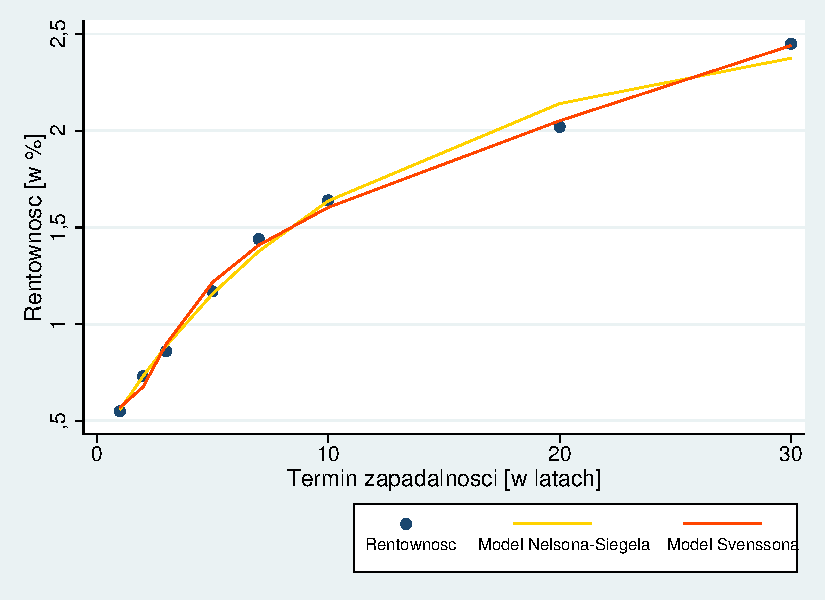
\includegraphics[height=4in]{Porownanie}
  \captionsetup{format=hang}
   \caption{Porównanie krzywych dochodowości amerykańskich obligacji skarbowych uzyskanych z~modelu Nelsona-Siegela i~modelu~Svenssona dla miesiąca czerwiec 2016}
\end{centering}
\begin{flushleft}
\hspace{1cm}\textit{\footnotesize{Źródło: Opracowanie własne.}} \\
\end{flushleft}
\end{figure}

Zaprezentowane powyżej modele posłużą w~bieżącej części rozdziału do wyznaczenia miesięcznych krzywych dochodowości. Ich komponenty zostały oszacowane przy pomocy Nieliniowej Metody Najmniejszych Kwadratów (ang. \textit{Non-linear Least Squares Method - NLSM}), przy parametrach początkowych: $\beta_0$ = 0, $\beta_1$ = 0, $\beta_2$ = 0, $\beta_3$ = 0, $\tau_1 = 1$, $\tau_2 = 1$. W~przypadku większości krzywych dochodowości wyznaczonych przez zaprezentowane powyżej modele lepiej dopasowane wizualnie okazały się krzywe uzyskane z~modelu Svenssona. Dobrym przykładem różnicy w~dopasowaniach modeli jest miesięczna krzywa dochodowości z~czerwca 2016~roku (\hyperlink{fig1}{wykres 1}). Jak wynika z~analizy powyższego wykresu krzywa uzyskana z~modelu Svenssona niemal idealnie przecina każdy z~punktów rentowności, krzywa wyliczona z~modelu Nelsona-Siegela nie jest tak dokładna. 

\vspace{0.25cm}
\hypertarget{fig2}{}
\begin{figure}[h]
\begin{centering}
  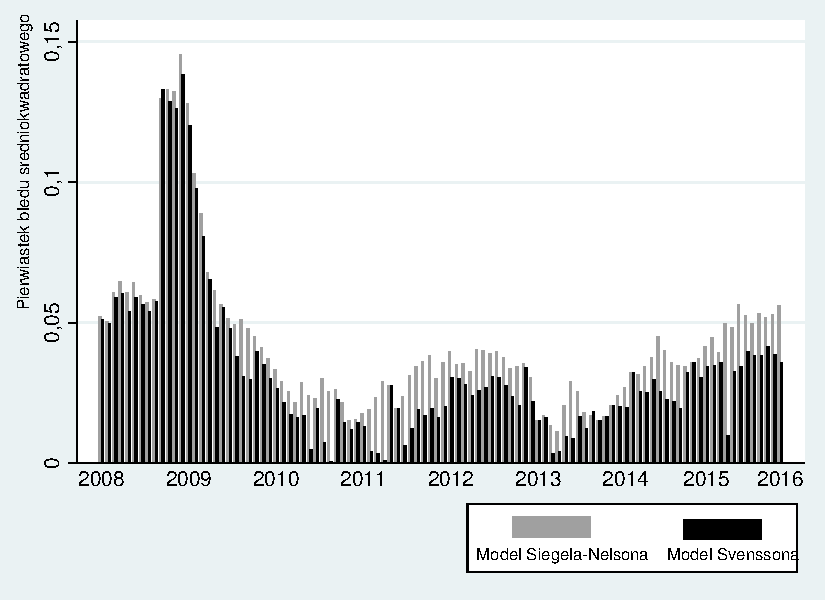
\includegraphics[height=4in]{RMSE}
  	\captionsetup{format=hang}
    \caption{Błędy RMSE uzyskane z~modelu Nelsona-Siegela i~modelu Svenssona dla krzywych dochodowości amerykańskich obligacji skarbowych w~latach 2008-2016}      
\end{centering}
\begin{flushleft}
\hspace{1cm}\textit{\footnotesize{Źródło: Opracowanie własne.}} \\
\end{flushleft}
\vspace{-0.5cm}
\end{figure}

Aby ostatecznie stwierdzić, który model jest lepiej dopasowany do sposobu kształtowania się rentowności obligacji skarbowych Stanów Zjednoczonych wyliczono pierwiastki błędów średniokwadratowych (ang. \textit{Root Mean Square Error - RMSE}) obu modeli zdefiniowane jako odchylenie krzywych wyestymowanych za pomocą analizowanych modeli od faktycznych rentowności (patrz \hyperlink{fig2}{wykres 2}). Kryterium minimalizacji pierwiastka błędu średniokwadratowego jednoznacznie wskazuje na konieczność wyboru modelu Svenssona, gdyż niemal w~całym badanym okresie (poza nielicznymi miesiącami) generuje on krzywe dochodowości z~niższym \acs{RMSE} niż model Nelsona-Siegela. Analizę wykresu pierwiastków błędów średniokwadratowych potwierdzają ich statystyki opisowe zaprezentowane w~\hyperlink{tab1}{tabeli 2}. Całkowita suma błędów \acs{RMSE}, ich średnia i~mediana jednoznacznie wskazują, że lepiej dopasowanym modelem do danych jest model Svenssona, jedynie nieznacznie niższe odchylenie standardowe mogłoby sugerować model Nelsona-Siegla. Aby sprawdzić czy średnie błędy \acs{RMSE} z~obu modeli istotnie się pomiędzy sobą różnią przeprowadzono test Manna-Whitneya-Wilcoxona (\acs{MWW}) na równość średnich w~próbkach niezależnych, który wykazał konieczność odrzucenia hipotezy zerowej o~równości średnich błędów \acs{RMSE} obu porównywanych modeli. Oznacza to, iż średnie błędy z~modelu Nelsona-Siegiela są istotnie wyższe niż średnie błędy z~modelu Svenssona. Biorąc pod uwagę zarówno analizę graficzną, statystyki opisowe, jak i~wynik testu statystycznego zdecydowano, iż do dalszych analiz przeprowadzanych w~tej pracy posłuży model Svenssona, jako model lepiej dopasowany do specyfiki amerykańskich papierów dłużnych. 

\hypertarget{tab1}{}
\begin{table}[!ht]
\rowcolors{2}{lightgray}{white}
\captionsetup{format=hang, position=top}
\caption{Statystyki opisowe błędów RMSE z~modelu Nelsona-Siegiela i modelu Svenssona oraz statystyka testowa MWW na równość średnich RMSE obu modeli}
\begin{tabular}{M{4.5cm}M{2.5cm}M{2.5cm}}
\toprule
\textbf{Cecha RMSE} & \textbf{Model_NS} & \textbf{Model_Svens}\\
\midrule
Suma & 4,3273 & 3,3884\\
Średnia & 0,0424 & 0,0332\\
Mediana & 0,0358 & 0,0268\\
Odchylenie Standardowe & 0,0262 & 0,0277\\
Statystyka testowa \acs{MWW} & \multicolumn{2}{c}{-3,966$^{***}$} \\
\bottomrule
\rowcolor{white!50}
\multicolumn{3}{m{10.5cm}}{\scriptsize Liczba gwiazdek wskazuje na jakim poziomie istotności należy odrzucić hipotezę zerową - w~przypadku testu Manna-Whitneya-Wilcoxona o~równości średnich w~próbkach niezależnych: 10\% ($^{*}$), 5\% ($^{**}$), 1\% ($^{***}$).}
\end{tabular}
\begin{flushleft}
\hspace{1cm}\textit{\footnotesize{Źródło: Opracowanie własne.}} \\
\end{flushleft}
\vspace{-0.5cm}
\end{table} 

\hyperlink{fig3}{Wykres 3} przedstawia kształtowanie się najważniejszych komponentów krzywej dochodowości obligacji skarbowych Stanów Zjednoczonych dla lat 2008-2016. Pierwszym istotnym komponentem krzywej dochodowości jest składnik krótkoterminowy ($\beta_0$ + $\beta_1$), oscylował on w~latach 2008-2011~wokół wartości -1\%, by w~kolejnych pięciu latach systematycznie rosnąć osiągając w~rezultacie wartość zbliżoną do 2\%. W~związku z~tym, iż sumę $\beta_0 + \beta_1$ interpretuje się jako bieżącą stopę oprocentowania lokaty overnight ($lim_{m->0}$ $R(m) = \beta_0$ + $\beta_1$) zachowanie tego wskaźnika może wskazywać, iż w~pierwszych trzech latach kryzysu Rezerwie Federalnej udało się utrzymać krótki koniec krzywej dochodowości na poziomie ujemnym, by w~kolejnych latach utracić wpływ na zachowanie się tego fragmentu krzywej dochodowości amerykańskich papierów dłużnych. 

\hypertarget{fig3}{}
\begin{figure}[h]
\vspace{0.25cm}
\begin{centering}
  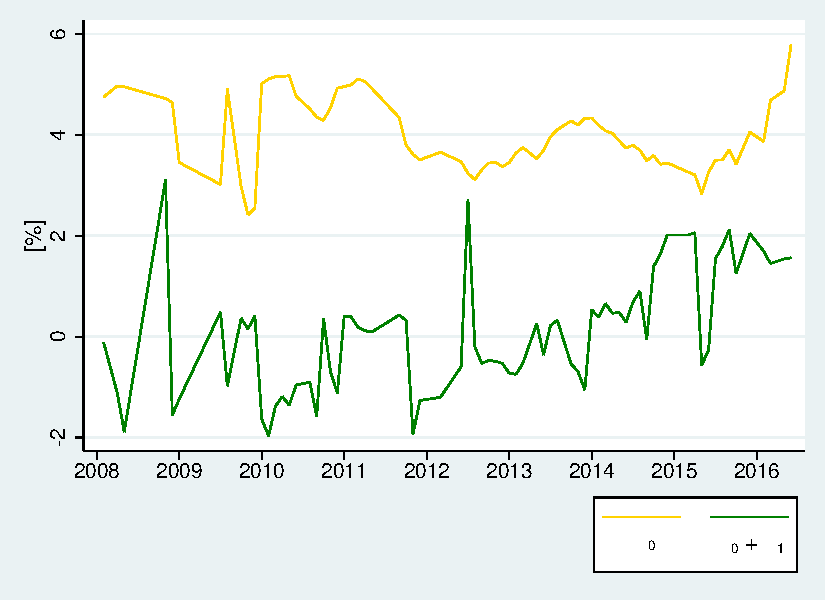
\includegraphics[height=4in]{Rysunki//Bety}
    \captionsetup{format=hang}
    \caption{Najważniejsze oszacowania krzywej dochodowości amerykańskich obligacji skarbowych wyliczone za pomocą modelu Svenssona dla lat 2008-2016}
\end{centering}
\begin{flushleft}
\hspace{1cm}\textit{\footnotesize{Źródło: Opracowanie własne.}} \\
\end{flushleft}
\vspace{-0.25cm}
\end{figure} 

Drugim istotnym komponentem krzywej dochodowości jest składnik długoterminowy $\beta_0$, który zgodnie z~\hyperlink{fig3}{wykresem 3}~początkowo oscylował wokół wartości równej 4\%, by od 2011~roku stopniowo ulegać osłabieniu osiągając w~połowie 2015~roku poziom zbliżony do 3\%. Z~kolei ostatnie dwa lata badania to dynamiczny wzrost parametru $\beta_0$ uwieńczony osiągnięciem poziomu zbliżonego do 6\%. Komponent $\beta_0$ interpretowany jest jako stopa, do której w~długim okresie dążą wszystkie stopy z~całej długości krzywej dochodowości ($lim_{m-> \infty}$ $R(m) = \beta_0$). Zachowanie tego parametru w~latach 2008-2016~może wskazywać, iż Rezerwie Federalnej udało się realnie obniżyć stopy długoterminowe dopiero po 2012~roku, czyli po ponad 3~latach stosowania luzowania ilościowego i~wydaniu blisko 2~bilionów dolarów. Obniżka ta została jednak odwrócona w~momencie, w~którym zaczęły się pojawiać pierwsze sygnały od członków \acs{FED} o~możliwym wyhamowaniu programu luzowania ilościowego. Kolejnym etapem badania będzie sprawdzenie, czy decyzje Rezerwy Federalnej miały faktyczny, statystycznie istotny, wpływ na kształt krzywej dochodowości obligacji skarbowych w~latach 2008-2016~wyznaczony za pomocą modelu Larsa E.O. Svenssona jako modelu najlepiej dopasowanego do danych.

\phantomsection	% do hiperlinków dla sekcji w spisie treści
\subsection*{\normalsize{3.1.2. Reakcja krzywej dochodowości na zmiany polityki monetarnej FED}}
\addcontentsline{toc}{subsection}{3.1.2. Reakcja krzywej dochodowości na zmiany polityki monetarnej FED}

W~badaniu reakcji krzywej dochodowości obligacji skarbowych Stanów Zjednoczonych na zmiany polityki monetarnej Rezerwy Federalnej postanowiono posłużyć się analizą graficzną średniomiesięcznych krzywych dochodowości wspartą testami na istotność różnic pomiędzy średnimi dziennymi rentownościami obligacji przed i~po ogłoszeniu komunikatu władz monetarnych (\textit{event study}). W~tym celu zidentyfikowano 10~najważniejszych komunikatów dotyczących niekonwencjonalnej polityki pieniężnej wygłoszonych przez członków amerykańskich władz monetarnych w~latach 2008-2016, które mogły istotnie wpłynąć na kształt krzywej dochodowości w~tym okresie. Daty tych wypowiedzi oraz ich skrócona treść zostały przedstawione w~\hyperlink{tab2}{tabeli 3}. 

Kolejnym etapem badania było sprawdzenie czy zaprezentowane w~\hyperlink{tab2}{tabeli 3} komunikaty istotnie wpłynęły, w~krótkim terminie, na kształt krzywej dochodowości reprezentowany przez średnie dzienne rentowności amerykańskich obligacji skarbowych. Założono w~tym momencie, iż już samo ogłoszenie zmian w~polityce monetarnej ma realny wpływ na oczekiwania uczestników rynku i~przejawia się za pomocą zmian rentowności obligacji skarbowych w~kolejnych dniach notowań następujących po ogłoszeniu komunikatu (kanał transmisji impulsów polityki monetarnej dotyczący oczekiwań uczestników rynku). Natomiast wdrożenie polityki (fizyczny skup aktywów) powinien być najlepiej odzwierciedlony w~zmianie kształtu krzywych dochodowości w~kolejnych miesiącach stosowania polityki (kanał pozostałych cen aktywów). 

Aby móc określić statystyczną istotność wpływu każdego z~przedstawionych w~\hyperlink{tab2}{tabeli 3}~komunikatów na średnie dzienne rentowności amerykańskich obligacji skarbowych przeprowadzono testy na równość średniej w~próbkach zależnych. Dla każdego z~komunikatów wydzielono dwa okna obserwacyjne - pierwsze z~obserwacjami poprzedzającymi, do miesiąca wstecz, komunikat (Okno 1) i~drugie z~obserwacjami następującymi1 do miesiąca po komunikacie, w~tym z~dnia komunikatu (Okno 2). Zastosowano tak wąskie okna obserwacji aby zapewnić, iż na poziomy rentowności obligacji w~tych oknach badawczych istotnie wpływać będą jedynie badane komunikaty (minimalny okres pomiędzy posiedzeniami \acs{FOMC} wynosi jeden miesiąc) a~nie inne wydarzenia rynkowe. W~rezultacie otrzymano po dwie próbki dla każdego komunikatu (przed i~po) zawierające po 21~obserwacji każda (średnia liczba dni notowań w~miesiącu). Obserwacje uzyskane w~próbkach reprezentują średni poziom rentowności dłużnych papierów skarbowych USA w~danym dniu notowań zdefiniowany jako średnia arytmetyczna z~rentowności obligacji o~ośmiu długościach od 1~roku do~30 lat (1-,~2-,~3-,~5-,~7-, 10-,~20-~i~30-letnie).

\hypertarget{tab2}{}
\begin{table}[H]
\rowcolors{2}{lightgray}{white}
\captionsetup{format=hang, position=top}
\caption{Daty i~skrócona treść najważniejszych komunikatów Rezerwy Federalnej dotyczących niekonwencjonalnej polityki monetarnej  w~latach 2008-2016}
\begin{tabular}{M{2.75cm}M{12.5cm}}
\toprule
\textbf{Data komunikatu} & \textbf{Skrócona treść komunikatu Rezerwy Federalnej}\\
\midrule
\hypertarget{kom1}{Komunikat 1:} 25.11.2008 & Ogłoszenie pierwszego programu luzowania ilościowego (\acs{QE}1) - plan zakupu: obligacji przedsiębiorstw sponsorowanych przez rząd (\acs{GSE}) o~wartości 100~miliardów dolarów oraz hipotecznych listów zastawnych (\acs{ABS}) o~wartości 500~miliardów.\cite{Fed09}   \\
\hypertarget{kom2}{Komunikat 2:} 18.03.2009 & Rozszerzenie program \acs{QE}1 - plan zakupu do końca marca 2010~roku 1,25~biliona hipotecznych listów zastawnych oraz 300~miliardów długoterminowych amerykańskich obligacji skarbowych.\cite{Fed10} \\
\hypertarget{kom3}{Komunikat 3:} 27.08.2010 & Szef Rezerwy Federalnej Ben Bernanke w~corocznej przemowie w~Jackson Hole wskazuje na możliwość przeprowadzenia kolejnego programu luzowanie ilościowego.\cite{bernanke11}\\
\hypertarget{kom4}{Komunikat 4:} 03.11.2010 & Ogłoszenie drugiego programu luzowania ilościowego (\acs{QE}2) - plan zakupu 600~miliardów amerykańskich długoterminowych obligacji skarbowych do końca czerwca 2011~roku.\cite{Fed12} \\
\hypertarget{kom5}{Komunikat 5:} 21.09.2011 & Ogłoszenie programu Operacja Twist - planu wydłużenie średniej duracji portfela \acs{FED} poprzez zakup do końca czerwca 2012~roku amerykańskich obligacji skarbowych o~wartości 400~miliardów dolarów z~zapadalnością od 6.~do~30. lat przy jednoczesnej sprzedaży obligacji krótszych niż trzyletnie o~takiej samej wartości.\cite{Fed13} \\
\hypertarget{kom6}{Komunikat 6:} 13.09.2012 & Ogłoszenie trzeciego programu luzowania ilościowego (\acs{QE}3) - plan regularnych, miesięcznych zakupów hipotecznych listów zastawnych o~wartości 40~miliardów dolarów bez określenia konkretnej daty zakończenia programu. Kontynuowanie operacji wydłużania duracji portfela obligacji skarbowych (\acs{OT}).\cite{Fed14}\\
\hypertarget{kom7}{Komunikat 7:} 12.12.2012 & Rozszerzenie programu \acs{QE}3 - poza kontynuowaniem regularnych zakupów hipotecznych listów zastawnych w~tempie 40~miliardów miesięcznie postanowiono dokonywać również zakupu długoterminowych amerykańskich obligacji skarbowych o~wartości 45~miliardów miesięcznie.\cite{Fed15}\\
\hypertarget{kom8}{Komunikat 8:} 19.06.2013 & Zapowiedź ograniczenia programu \acs{QE}3 (ang. \textit{Taper Tantrum - TT}) - wypowiedź przewodniczącego Rezerwy Federalnej sugerująca możliwość ograniczenia tempa skupu aktywów ze względu na poprawiająca się sytuację ekonomiczną amerykańskiej gospodarki (rozpoczęcie procesu wycofywania się z~niekonwencjonalnej polityki pieniężnej).\cite{bernanke18}\\
\hypertarget{kom9}{Komunikat 9:} 18.12.2013 & Rozpoczęcie ograniczania programu \acs{QE}3 - plan zmniejszania miesięcznej wartości kupowanych aktywów o~10 miliardów dolarów na każdym posiedzeniu w~2014 roku.\cite{Fed16}\\
\hypertarget{kom10}{Komunikat 10:} 29.10.2014 & Ostateczne zakończenie trzeciego programu luzowania ilościowego po zgromadzeniu papierów wartościowych o~wartości blisko 4,5~biliona dolarów w~bilansie Rezerwy Federalnej.\cite{Fed17}\\
\bottomrule
\end{tabular}
\begin{flushleft}
\hspace{1cm}\textit{\footnotesize{Źródło: Opracowanie własne.}} \\
\end{flushleft}
\vspace{-0.5cm}
\end{table} 

Większość uzyskanych próbek pochodziło z~rozkładu normalnego, badanego przy pomocy testu Shapiro-Wilka (\acs{SW}) odpowiedniego dla małych prób nieprzekraczających 50~obserwacji. Wyjątek stanowił okres 21 dni po ogłoszeniu \hyperlink{kom10}{komunikatu nr 10}, który okazał się nie posiadać rozkładu zbliżonego do normalnego. Dla tak zdefiniowanych próbek przeprowadzono testy: parametryczny test T~oraz nieparametryczny test Wilcoxona.

\vspace{0.25cm}
\hypertarget{tab3}{}
\begin{table}[!ht]
\rowcolors{4}{lightgray}{white}
\captionsetup{format=hang, position=top}
\caption{Statystyki testowe testów na normalność (SW) oraz na równość średnich w~próbach zależnych (T-Test i~Wilcoxon), a~także zmiana średniej rentowności dla 10~najważniejszych komunikatów Rezerwy Federalnej z~lat 2008-2016}
\begin{tabular}{
M{2.5cm}
S[table-format=3.3,table-space-text-post=$^{***}$]
S[table-format=3.3,table-space-text-post=$^{***}$]
S[table-format=3.3,table-space-text-post=$^{***}$]
S[table-format=3.3,table-space-text-post=$^{***}$]
M{2.5cm}
}
\toprule
\textbf{Numer} & \textbf{Statystyka} & \textbf{Statystyka} & \textbf{Statystyka} & \textbf{Statystyka} & \textbf{Zmiana}\\
\textbf{komunikatu} & {\textbf{testowa}} & {\textbf{testowa}} & {\textbf{testowa}} & {\textbf{testowa}} & \textbf{średniej}\\
\textbf{FED} & {\textbf{SW (Okno 1)}} & {\textbf{SW (Okno 2)}} & {\textbf{T-Test}} & {\textbf{Wilcoxon}}& \textbf{rentowności}\\
\midrule
Komunikat 1  & 0,914$^{*}$ &  0,953 &  24,932$^{***}$ &    4,015$^{***}$  &    {-86 p.b.}\\
Komunikat 2  &  0,947 &  0,970 &   5,236$^{***}$ &    3,493$^{***}$  &    {-10 p.b.}\\
Komunikat 3  & 0,946 & 0,983 &   2,307$^{**}$  &    1,547          &      {-}\\
Komunikat 4  &  0,963 & 0,921$^{*}$ & -10,122$^{***}$ &   -3,998$^{***}$  &    {+21 p.b.}\\
Komunikat 5  &  0,954 & 0,937 &   1,495         &    1,373          &        {-} \\
Komunikat 6  & 0,943 & 0,951 &  -1,282         &   -1,269          &        {-} \\
Komunikat 7  & 0,962 & 0,948 & -10,307$^{***}$ &   -4,015$^{***}$  &    {+12 p.b.}\\
Komunikat 8  &  0,914$^{*}$ & 0,953 & -17,909$^{***}$ &   -4,015$^{***}$  &    {+24 p.b.}\\
Komunikat 9  & 0,943 &  0,915$^{*}$ &  -7,474$^{***}$ &   -4,015$^{***}$  &    {+11 p.b.}\\
Komunikat 10 & 0,953 & 0,866$^{***}$ &  {-}    &   -1,251          &          {-} \\
\bottomrule
\multicolumn{6}{m{15cm}}{\scriptsize Liczba gwiazdek wskazuje na jakim poziomie istotności należy odrzucić hipotezę zerową - w~przypadku testu Shapiro-Wilka o~normalności rozkładu, w~przypadku T-Testu i~Wilcoxona o~równości średnich w~próbkach zależnych: 10\% ($^{*}$), 5\% ($^{**}$), 1\% ($^{***}$).}
\end{tabular}
\begin{flushleft}
\textit{\footnotesize{Źródło: Opracowanie własne.}} \\
\end{flushleft}
\vspace{-0.35cm}
\end{table} 

Wyniki testów na równość średnich w~próbkach zależnych zostały zaprezentowane w~\hyperlink{tab3}{tabeli 4}. Jej analiza wskazuje na statystyczną istotność na 99\%-owym poziomie ufności sześciu komunikatów: \hyperlink{kom1}{1}, \hyperlink{kom2}{2}, \hyperlink{kom4}{4}, \hyperlink{kom7}{7}, \hyperlink{kom8}{8} oraz \hyperlink{kom9}{9}. \hyperlink{kom3}{Trzeci komunikat} okazał się istotny na 95\%-owym poziomie istotności tylko w~teście T, dlatego też nie został w~niniejszej pracy uznany za istotnie wpływający na kształt krzywej dochodowości. Dla komunikatów \hyperlink{kom5}{5.} i~\hyperlink{kom6}{6.} oba testy wskazały na brak konieczności odrzucenia hipotezy zerowej o~równości średnich w~próbkach zależnych na akceptowalnym poziomie istotności (5\%) - co oznacza, iż nie wpłynęły one istotnie na średnią rentowność amerykańskich obligacji skarbowych. Dla \hyperlink{kom10}{komunikatu 10.} ze względu na brak normalności jednej z~próbek można było przeprowadzić tylko test Wilcoxona, wskazał on na brak konieczności odrzucenia hipotezy zerowej o~równości średniej w~próbkach zależnych na akceptowalnym poziomie istotności - komunikat okazał się statystycznie nieistotny. 

\hyperlink{tab3}{Tabela 4}~poza statystykami testowymi prezentuje również skalę zmiany średniej rentowności dla komunikatów statystycznie istotnych. Jak wynika z~tabeli tylko dwa pierwsze komunikaty wpłynęły istotnie na natychmiastowy spadek średniej rentowności amerykańskich obligacji skarbowych. Tymi komunikatami było rozpoczęcie pierwszego luzowania ilościowego (-86~p.b.) oraz jego rozszerzenie (-10~p.b.) - co jest zgodne z~obserwacjami przedstawionymi w~artykule J. Gagnon, M. Raskin, J.Remache oraz B. Sack \cite{gagnon34}, omówionym w drugim rozdziale niniejszej pracy. Pozostałe komunikaty przedstawione w~\hyperlink{tab3}{tabeli 3} albo okazały się statystycznie nieistotne albo wpłynęły na nieznaczny wzrost średnich rentowności przynajmniej w~krótkoterminowej perspektywie. Jest to całkowicie zrozumiałe w~przypadku informacji o~ograniczeniu skali zakupów obligacji skarbowych (komunikaty \hyperlink{kom8}{8} i~\hyperlink{kom9}{9}) jednak zapowiedzi rozszerzenia skali niekonwencjonalnych programów (komunikaty \hyperlink{kom4}{4} i~\hyperlink{kom7}{7}) powinny prowadzić do spadku rentowności amerykańskich obligacji skarbowych. 

\vspace{0.25cm}
\hypertarget{fig4}{}
\begin{figure}[h]
\begin{centering}
  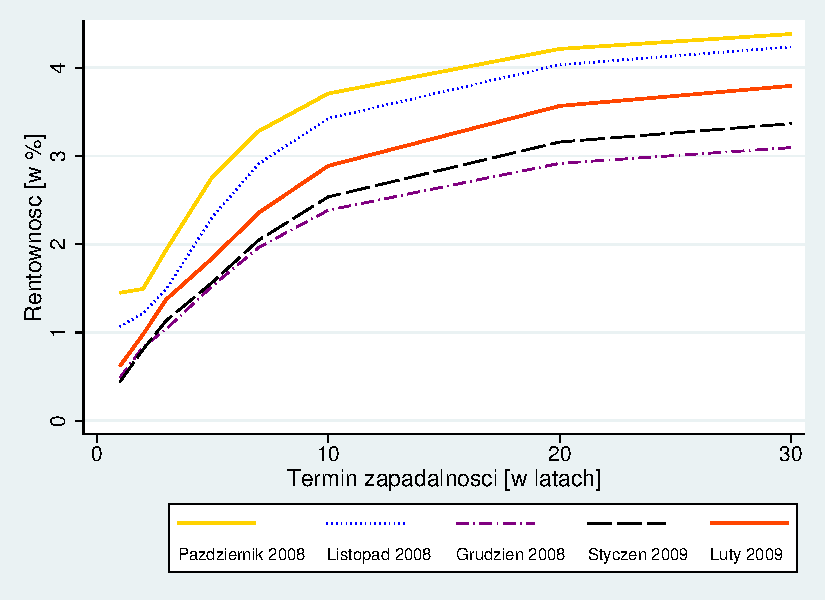
\includegraphics[height=4in]{krzywa1}
    \captionsetup{format=hang}
    \caption{Reakcja krzywej dochodowości na ogłoszenie \protect\hyperlink{kom1}{komunikatu 1} (rozpoczęcie QE1)}
\end{centering}
\begin{flushleft}
\hspace{1cm}\textit{\footnotesize{Źródło: Opracowanie własne.}} \\
\end{flushleft}
\vspace{-0.5cm}
\end{figure}

Po zbadaniu krótkoterminowej reakcji krzywej dochodowości na ogłaszanie kolejnych programów niekonwencjonalnej polityki pieniężnej w~dalszej analizie skupiono się na kształcie krzywych dochodowości w~nieco dłuższym, trzymiesięcznym okresie, odnosząc swe analizy do miesiąca poprzedzającego miesiąc ogłoszenia komunikatu. \hyperlink{fig4}{Wykres 4}~prezentuje kształt krzywej dochodowości dla miesiąca poprzedzającego decyzję Rezerwy Federalnej o~rozpoczęciu pierwszego programu luzowania ilościowego oraz krzywe z~kolejnych czterech miesięcy następujących po ogłoszeniu \hyperlink{kom1}{komunikatu 1}. Z~wykresu wynika, iż ogłoszenie zastosowania niekonwencjonalnej polityki pieniężnej mogło spowodować wyraźne spłaszczenie się krzywej dochodowości w~perspektywie 4~miesięcy na całej jej długości od o~około 50~punktów bazowych na krótkim jej końcu aż do 1~punktu procentowego w~jej dalszym fragmencie\footnote{Warto w~tym miejscu wspomnieć, że 16.~grudniu 2008 roku amerykańskie władze monetarne postanowiły zakończyć trwającą od sierpnia 2007 roku serię obniżek stopy funduszy federalnych ustanawiając dla niej przedział 0\%-0,25\%, co mogło mieć najsilniejszy wpływ na krótki koniec krzywej dochodowości.}. Wnioski te pokrywają się z~analizą przedstawioną we wcześniejszym fragmencie rozdziału gdzie krótkoterminowy wpływ \hyperlink{kom1}{komunikatu 1} na średnią rentowność wynosił około -84~punkty bazowe - w~perspektywie 4~miesięcy wpływ ten spadł do -73~punktów bazowych.

\vspace{0.25cm}
\hypertarget{fig5}{}
\begin{figure}[h]
\begin{centering}
  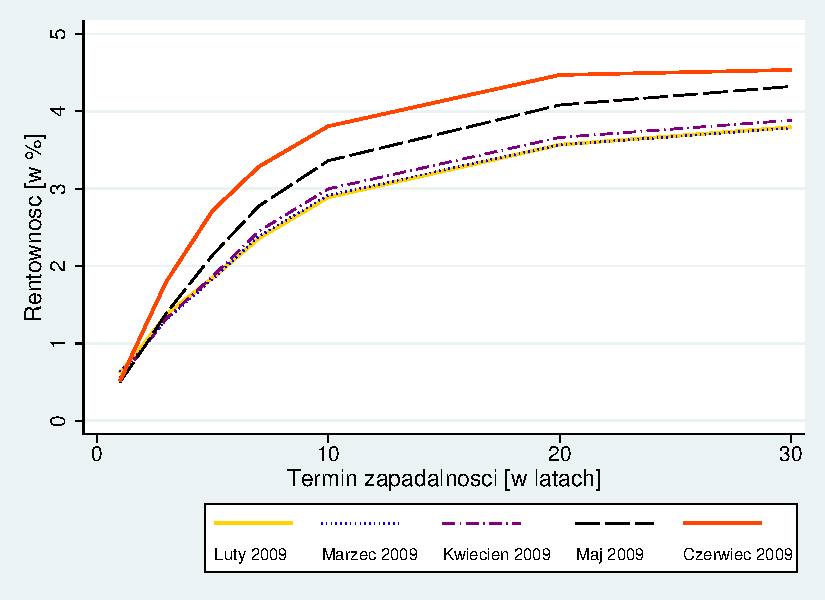
\includegraphics[height=4in]{krzywa2}
    \captionsetup{format=hang}
    \caption{Reakcja krzywej dochodowości na ogłoszenie \protect\hyperlink{kom2}{komunikatu 2} (rozszerzenie QE1)}
\end{centering}
\begin{flushleft}
\hspace{1cm}\textit{\footnotesize{Źródło: Opracowanie własne.}} \\
\end{flushleft}
\vspace{-0.5cm}
\end{figure}

Ogłoszenie komunikatu o~rozszerzeniu pierwszego programu luzowania ilościowego 18. marca 2009~roku przynosi zupełnie inne obserwacje (\hyperlink{fig5}{wykres 5}). Analiza \hyperlink{fig5}{wykresu 5} wskazuje, iż ogłoszenie \hyperlink{kom2}{komunikatu 2} mogło co najwyżej chwilowo wyhamować obserwowane od stycznia 2009~wzrosty rentowności amerykańskich obligacji skarbowych (-10 b.p reakcji dziennych krzywych), które już w~czerwcu 2009~wróciły do poziomów z~października 2008. Taka reakcja krzywej dochodowości wydaje się sprzeczna z~oczekiwaniami - ogłoszenie bezprecedensowego planu zakupu przez Rezerwę Federalną długoterminowych amerykańskich obligacji skarbowych o~wartości 300~miliardów dolarów powinno wyraźnie wzmocnić popyt rynkowy i~bezpośrednio wpłynąć na wzrost cen obligacji~a tym samym na obniżenie ich rentowności. Nie miało to jednak miejsca - rentowności w~kolejnych miesiącach wzrastały nie zważając na znaczące zakupy amerykańskich obligacji skarbowych przez Rezerwę Federalną.

\vspace{0.25cm}
\hypertarget{fig6}{}
\begin{figure}[h]
\begin{centering}
  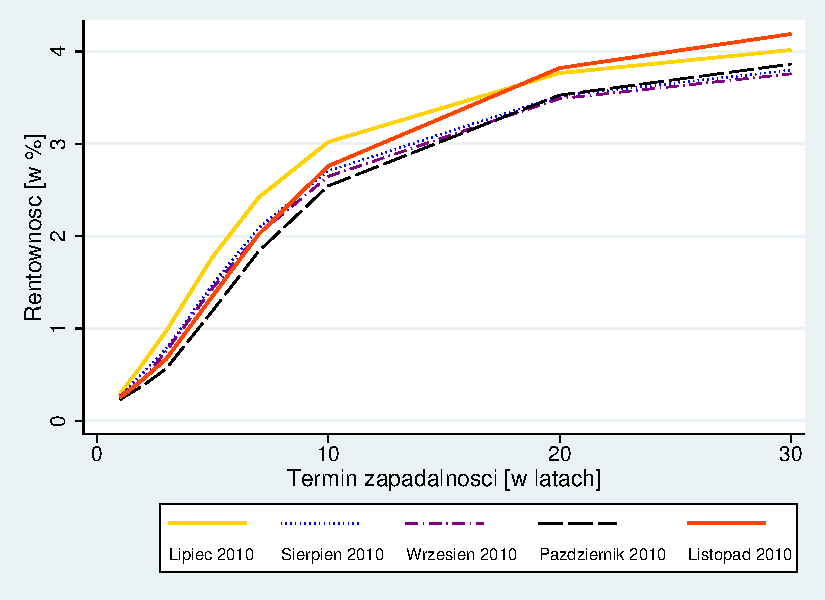
\includegraphics[height=4in]{krzywa3}
    \captionsetup{format=hang}
    \caption{Reakcja krzywej dochodowości na ogłoszenie \protect\hyperlink{kom3}{komunikatu 3} (zapowiedź QE2)}
\end{centering}
\begin{flushleft}
\hspace{1cm}\textit{\footnotesize{Źródło: Opracowanie własne.}} \\
\end{flushleft}
\vspace{-0.5cm}
\end{figure}

\hyperlink{fig6}{Wykres 6}~potwierdza wnioski płynące z~analizy dziennych rentowności - od lipca 2010~roku do listopada 2010~roku krzywa dochodowości praktycznie nie zmieniła swojego kształtu poza delikatnym spłaszczeniem się (około -10 punktów bazowych) we fragmencie pomiędzy rokiem a~dziesięcioma latami. Mogłoby to wskazywać, iż \hyperlink{kom3}{komunikat 3} był neutralny dla uczestników rynku dłużnych papierów skarbowych w~Stanach Zjednoczonych. Co oznacza, iż albo został on ujęty wcześniej w~cenach, albo obserwacje pierwszego programu luzowania ilościowego kazały sądzić inwestorom, iż drugi taki program nie będzie miał znaczącego wpływu na rynek.

\vspace{0.5cm}
\hypertarget{fig7}{}
\begin{figure}[H]
\centering
\captionsetup{format=hang}
\caption{Reakcje krzywych dochodowości na ogłoszenie komunikatów \protect\hyperlink{kom4}{4} oraz \protect\hyperlink{kom5}{5}}
\begin{subfigure}{.5\textwidth}
\hspace{-3cm}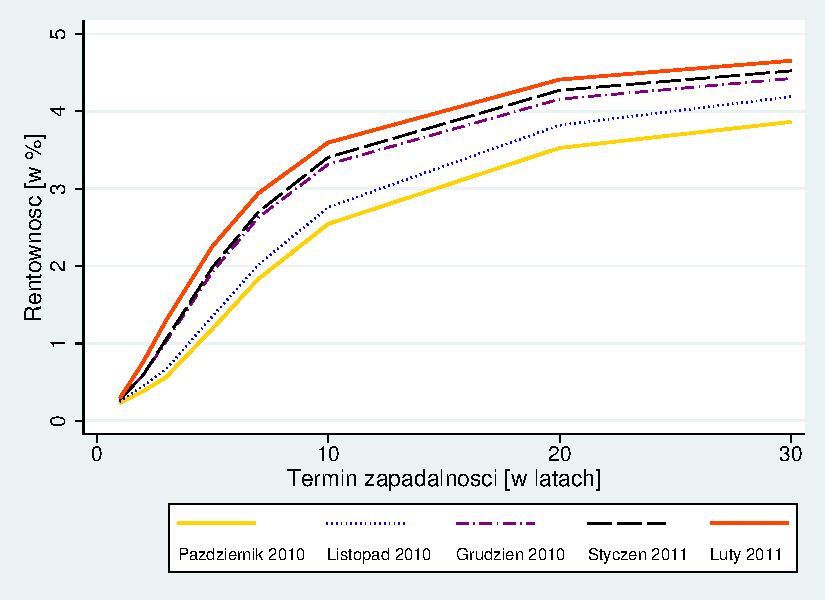
\includegraphics[height=4in]{krzywa4}
 \caption{\protect\hyperlink{kom4}{Komunikat 4} (rozpoczęcie QE2)}
\hypertarget{fig7}{}
\vspace*{\floatsep} % przerwa między wykresami
\end{subfigure}
\begin{subfigure}{.5\textwidth}
\hspace{-3cm}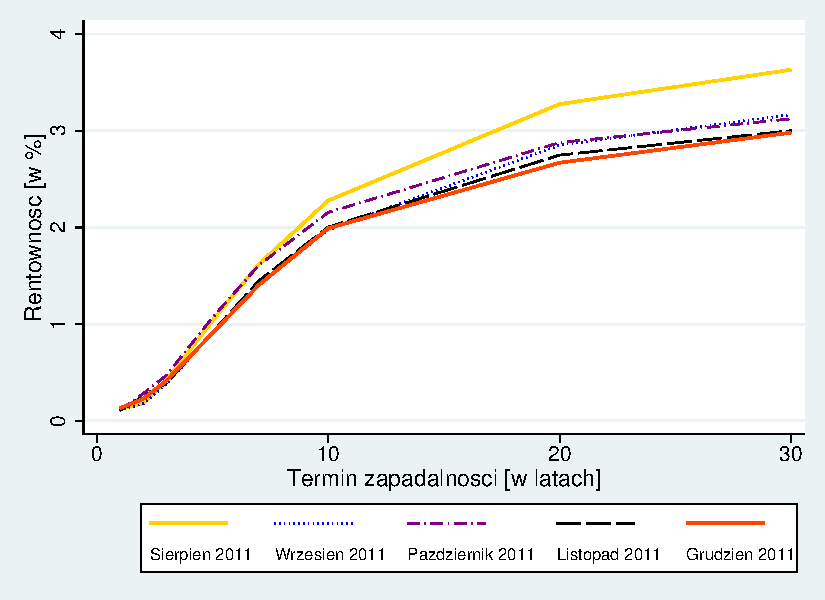
\includegraphics[height=4in]{krzywa5}
\caption{\protect\hyperlink{kom5}{Komunikat 5} (rozpoczęcie OT)}
\end{subfigure}
\begin{flushleft}
\hspace{1cm}\textit{\footnotesize{Źródło: Opracowanie własne.}} \\
\end{flushleft}
\vspace{-0.5cm}
\end{figure}

Na \hyperlink{fig7}{wykresie 7}~zaprezentowane są krzywe dochodowości w~kolejnych miesiącach po ogłoszeniu komunikatów \hyperlink{kom4}{4} i~\hyperlink{kom5}{5}. W~obu przypadkach potwierdzają się wnioski płynące z~analizy zmian dziennych rentowności. Tuż po rozpoczęciu \acs{QE}2 krzywa dochodowości wzrosła o~około 25~p.b. by do lutego 2011~roku wzrosnąć o~kolejne 50~p.b. Rozpoczęcie operacji Twist nie wpłynęło istotnie na rentowności obligacji skarbowych, widać jedynie ich delikatny spadek (-20 p.b.) na długim końcu krzywej w~stosunku do miesiąca przed ogłoszeniem tego programu.

\vspace{0.25cm}
\hypertarget{fig8}{}
\begin{figure}[h]
\begin{centering}
  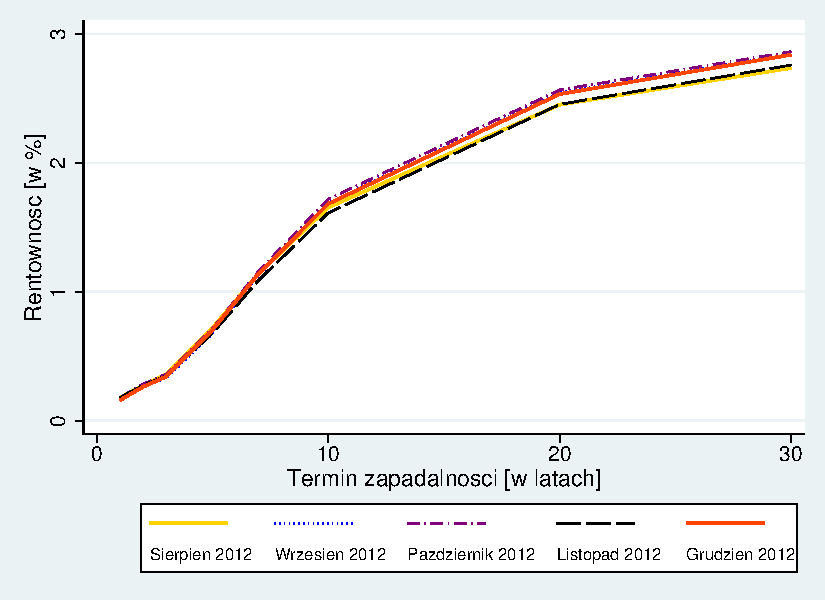
\includegraphics[height=4in]{krzywa6}
    \captionsetup{format=hang}
    \caption{Reakcja krzywej dochodowości na ogłoszenie \protect\hyperlink{kom6}{komunikatu 6} (rozpoczęcie QE3)}
\end{centering}
\begin{flushleft}
\hspace{1cm}\textit{\footnotesize{Źródło: Opracowanie własne.}} \\
\end{flushleft}
\vspace{-0.5cm}
\end{figure}

Wnioski płynące z~analizy \hyperlink{fig8}{wykresu 8} są tożsame z~wnioskami płynącymi z~analizy wpływu \hyperlink{kom6}{komunikatu 6} na dzienne rentowności obligacji skarbowych - kształt krzywej dochodowości pozostawał praktycznie bez zmian pomiędzy sierpniem 2012~a grudniem 2012~pomimo ogłoszenia kolejnego, trzeciego już, programu luzowania ilościowego. Brak reakcji krzywej dochodowości może tłumaczyć fakt, iż \acs{QE}3~początkowo zakładało skup hipotecznych listów zastawnych w~tempie 40~miliardów dolarów miesięcznie, a~nie bezpośrednio obligacji skarbowych. Kontynuowana była jednak program wydłużania duracji portfela Rezerwy Federalnej, który w~intencji amerykańskich władz monetarnych miał wywoływać spadek rentowności długoterminowych obligacji skarbowych.

\vspace{0.5cm}
\hypertarget{fig9}{}
\begin{figure}[H]
\centering
\captionsetup{format=hang}
\caption{Reakcje krzywych dochodowości na ogłoszenie komunikatów \protect\hyperlink{kom7}{7} oraz \protect\hyperlink{kom8}{8}}
\begin{subfigure}{.5\textwidth}
\hspace{-3cm}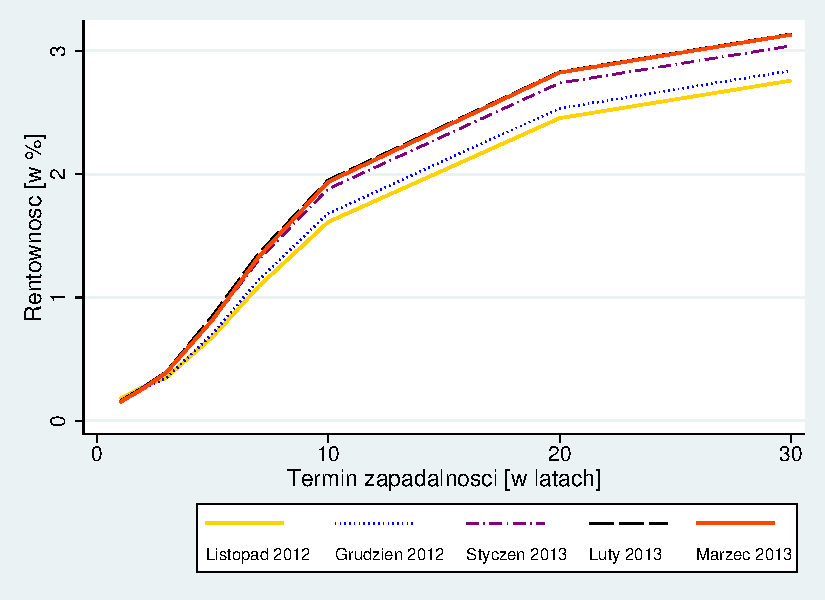
\includegraphics[height=4in]{krzywa7}
 \caption{\protect\hyperlink{kom7}{Komunikat 7} (rozszerzenie QE3)}
\hypertarget{fig10}{}
\vspace*{\floatsep} % przerwa między wykresami
\end{subfigure}
\begin{subfigure}{.5\textwidth}
\hspace{-3cm}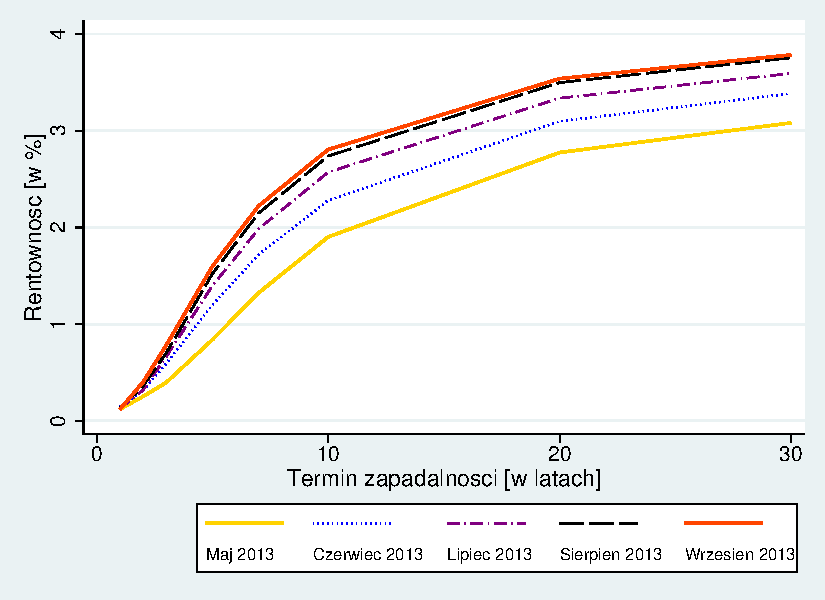
\includegraphics[height=4in]{krzywa8}
\caption{\protect\hyperlink{kom8}{Komunikat 8} (zapowiedź ograniczenia QE3)}
\end{subfigure}
\begin{flushleft}
\hspace{1cm}\textit{\footnotesize{Źródło: Opracowanie własne.}} \\
\end{flushleft}
\vspace{-0.5cm}
\end{figure}

Krzywe dochodowości po ogłoszeniu komunikatów \hyperlink{kom7}{7} i~\hyperlink{kom8}{8} kształtowały się bardzo podobnie (patrz \hyperlink{fig9}{wykresu 9}), pomimo, iż pierwszy z~nich dotyczył rozszerzenia skali zakupów obligacji skarbowych, a~drugi zapowiadał ich ograniczenie. Obie krzywe odnotowały wzrosty pierwsza o~około 30~p.b. a~druga o~około 50~p.b. z~tym, że w~przypadku tej drugiej wzrosty były dużo wyraźniejsze dla rentowności od roku do dziesięciu lat. 

\vspace{0.25cm}
\hypertarget{fig11}{}
\begin{figure}[h]
\begin{centering}
  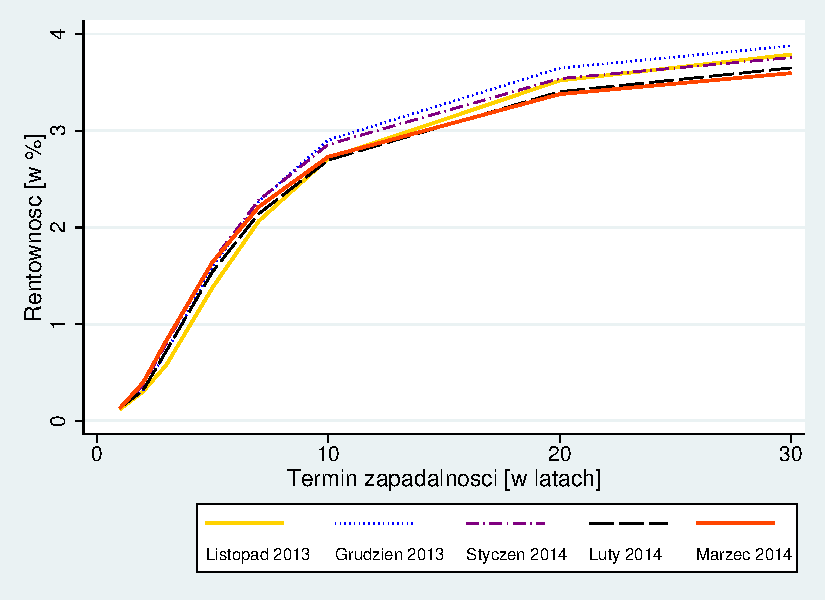
\includegraphics[height=4in]{krzywa9}
    \captionsetup{format=hang}
    \caption{Reakcja krzywej dochodowości na ogłoszenie \protect\hyperlink{kom9}{komunikatu 9} (ograniczenie QE3)}
\end{centering}
\begin{flushleft}
\hspace{1cm}\textit{\footnotesize{Źródło: Opracowanie własne.}} \\
\end{flushleft}
\vspace{-0.5cm}
\end{figure}

Wbrew wnioskom płynącym z~pierwszej części podrozdziału, wydaje się, iż ogłoszenie \hyperlink{kom9}{komunikatu 9} nie odcisnęło swojego piętna na kształcie krzywej dochodowości - rentowności z~okresu listopad 2013 - marzec 2014~nie uległy zbyt istotnym zmianom. Badanie reakcji krótkoterminowej wskazywało na nieznaczny wzrost o~około~11~p.b., który jest również zauważalny na \hyperlink{fig11}{wykresie 10}, jednak w~kolejnych miesiącach wzrost ten został całkowicie zniwelowany przez delikatne spłaszczenie się krzywej dochodowości. Można by domniemywać, iż ten komunikat był spodziewany przez rynek z~powodu kilku wcześniejszych wypowiedzi przewodniczącego Rezerwy Federalnej i~został ujęty już wcześniej w~wycenach amerykańskich obligacji skarbowych, dlatego też nie wywołał tak znaczącego efektu jak wcześniejsze zapowiedzi.\\

\vspace{0.25cm}
\hypertarget{fig12}{}
\begin{figure}[h]
\begin{centering}
  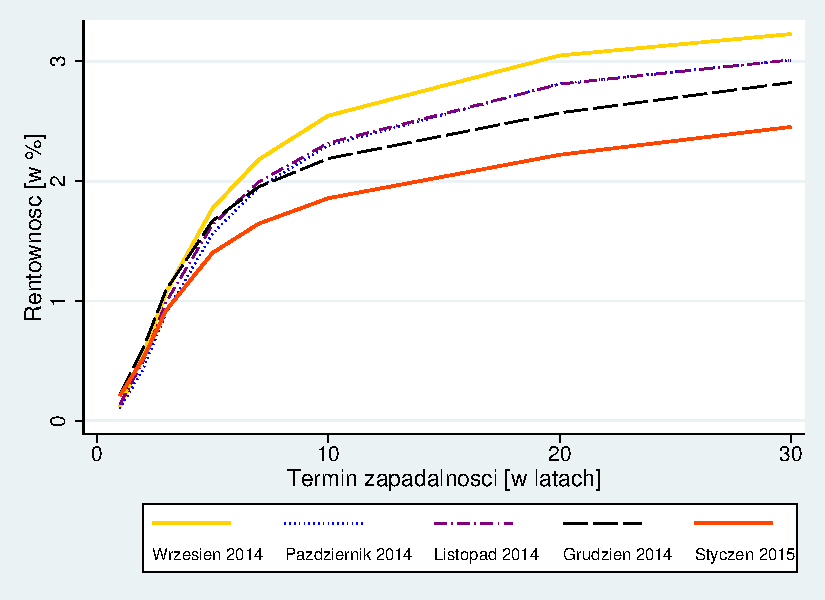
\includegraphics[height=4in]{krzywa10}
    \captionsetup{format=hang}
    \caption{Reakcja krzywej dochodowości na ogłoszenie \protect\hyperlink{kom10}{komunikatu 10} (zakończenie QE3)}
\end{centering}
\begin{flushleft}
\hspace{1cm}\textit{\footnotesize{Źródło: Opracowanie własne.}} \\
\end{flushleft}
\vspace{-0.5cm}
\end{figure}

Pomimo braku istotności \hyperlink{kom10}{komunikatu 10} w~kontekście krótkoterminowego wpływu na średnie dzienne rentowności, istotności tego komunikatu można domniemywać patrząc na dłuższą perspektywę czasową. Na \hyperlink{fig12}{wykresie 11} widać istotną zmianę (około -50~p.b.) rentowności amerykańskich obligacji skarbowych pomiędzy wrześniem 2014~a~styczniem 2015, jednak kierunek tej zmiany jest inny niż można by się spodziewać -  trzy miesiące po zakończeniu bezprecedensowego skupu długoterminowych aktywów krzywa dochodowości osiągnęła na swym dłuższym krańcu niższy poziom niż w~którymkolwiek momencie stosowania niekonwencjonalnej polityki pieniężnej. Mogło to być spowodowane czynnikami zupełnie nie związanymi z~polityką monetarną Rezerwy Federalnej, a~generalnym wzrostem niepewności na rynkach finansowych spowodowanym kolejną odsłoną kryzysu zadłużeniowego w~Grecji i~związaną~z~tym~ucieczką inwestorów do tak zwanych "bezpiecznych przystani"\footnote{Bezpieczna przystań (ang. \textit{safe haven}) to aktywo finansowe, które w~czasie turbulencji na globalnych rynkach finansowych zachowuje swoją wartość, gwarantując inwestorom minimalne ryzyko kosztem minimalnego zysku lub niewielkiej straty}, jakimi niewątpliwie są amerykańskie papiery skarbowe.

Analiza graficzna wykresów miesięcznych krzywych dochodowości nie przynosi jednoznacznych wniosków co do skuteczności decyzji Rezerwy Federalnej w~kształtowaniu krzywej dochodowości amerykańskich obligacji skarbowych. Można zaobserwować wyraźną różnicę pomiędzy reakcją krzywych dochodowości w~najważniejszych momentach stosowania programu pierwszego luzowania ilościowego, a~reakcją w~podobnych momentach dla pozostałych programów - w~przypadku \acs{QE}1 rentowności obligacji zdają się reagować silniej, reakcje te są statystycznie istotne i~są zgodne z~intencją Rezerwy Federalnej. Porównywalne reakcje wywoływały tylko zapowiedzi wskazujące na zakończenie stosowania niekonwencjonalnej polityki monetarnej. W~większości przypadków bezpośrednio po ogłoszeniu komunikatu o~zmianie polityki pieniężnej krzywe dochodowości reagowały wzrostem często wbrew deklarowanym intencjom amerykańskich władz monetarnych i~wzrosty te były następnie kontynuowane w~kolejnych miesiącach\footnote{Opisywane zmiany rentowności długoterminowych obligacji skarbowych Stanów Zjednoczonych są sprzeczne z~wioskami płynącymi z~analizy literatury badawczej przedstawionej w~rozdziale drugim, gdzie stwierdzono statystyczną istotność wpływu niekonwencjonalnej polityki monetarnej na obniżenie rentowności amerykańskich papierów dłużnych.}. O~ile takie zachowanie rynku można by spróbować wytłumaczyć, w~początkowym etapie kryzysu gospodarczego (lata 2008-2009), wyjątkowo wysokim poziomem zmienności rynków finansowych, o tyle po 2009~roku takie wytłumaczenie nie ma racjonalnych przesłanek. Na początku 2010~roku problemy finansowe Grecji rozpoczęły kryzys zadłużeniowy w~strefie euro, amerykańskie obligacje umocniły swoją pozycję jako bezpieczna przystań dla inwestorów, co powinno wywołać presję na wzrost ich cen i~spadek rentowności - w~efekcie wspomagając niekonwencjonalną politykę pieniężną prowadzoną przez Rezerwę Federalną. Nie miało to jednak miejsca - rentowności amerykańskich obligacji skarbowych w~okresie 2010-2Q2016 wahały się w~tunelu [0,25\%; 3-4,5\%] bez wyraźnego trendu. Możliwe więc, iż popyt na rynku dłużnych papierów skarbowych, w~momencie gdy zmalała niepewność związana z~kryzysem w~Stanach Zjednoczonych, został częściowo zniwelowany przez okazje inwestycyjne na innych rynkach finansowych (akcyjnym, nieruchomości, surowcowym) lub też pieniądze z~tego rynku trafiały bezpośrednio do przedsiębiorców realizujących projekty biznesowe i~w ten sposób napędzały amerykańską gospodarkę (co byłoby zgodne z~intencją Rezerwy Federalnej). Wyjaśniałoby to reakcję krzywej dochodowości na ogłaszanie kolejnych niekonwencjonalnych programów po \acs{QE}1 (wzrosty rentowności). Programy te mogły być impulsem do kolejnych odpływów kapitału z~rynków dłużnych papierów wartościowych ku rynkom obarczonym większym ryzykiem. Byłoby to częściowo zgodne z~obserwacjami zawartymi w~literaturze badawczej, gdzie odnotowano wpływ niekonwencjonalnej polityki monetarnej na wzrost cen akcji (\cite{chen36}/\cite{bhattarai36}/\cite{swanson37}). Warto zbadać tę hipotezę sprawdzając wpływ działań amerykańskich władz monetarnych nie tylko na krzywą dochodowości ale także na wskaźniki reprezentujące inne segmenty gospodarki Stanów Zjednoczonych. Tego właśnie dotyczyć będzie następny podrozdział niniejszej pracy.

\hypertarget{podrz32}{}
\phantomsection	% do hiperlinków dla sekcji w spisie treści
\section*{\large{3.2. Skuteczność w~oddziaływaniu na wybrane sektory amerykańskiej gospodarki}}
\addcontentsline{toc}{section}{3.2. Skuteczność w~oddziaływaniu na wybrane sektory amerykańskiej gospodarki}

W~tej części pracy przeprowadzone zostanie badanie empiryczne wpływu niekonwencjonalnej polityki monetarnej Rezerwy Federalnej na amerykańską gospodarkę w~latach 2008-2016. Będzie to próba rozszerzenia badania przeprowadzonego w~poprzedniej części pracy o~zmienne reprezentujące inne segmenty gospodarki Stanów Zjednoczonych niż tylko rynek dłużnych papierów skarbowych. Wydłużony zostanie też horyzont badanego wpływu - w~poprzednim rozdziale był to horyzont od kilkudziesięciu dni (testy istotności) do 5~miesięcy (analiza graficzna kształtu krzywej dochodowości) - w~tym rozdziale horyzontem badawczym będzie rok, czyli średni czas trwania niekonwencjonalnych programów stosowanych przez Rezerwę Federalną. Aby to osiągnąć wykorzystany zostanie model wektorowej autoregresji. W~pierwszej fazie przedstawiony zostanie krótki opis zmiennych wykorzystanych w~badaniu, następnie nakreślona zostanie specyfikacja modelu \acs{VAR} wraz z~jego testami diagnostycznymi, a~na końcu opisane zostaną najważniejsze wnioski wypływające z~modelu, skupiając się w~szczególności na analizie funkcji odpowiedzi na impuls, dekompozycji wariancji prognoz oraz na samych prognozach.

\phantomsection% do hiperlinków dla sekcji w spisie treści
\subsection*{\normalsize{3.2.1. Opis zbioru danych i~specyfikacja modelu}}
\addcontentsline{toc}{subsection}{3.2.1. Opis zbioru danych i~specyfikacja modelu}
\vspace{0.4cm}

Konstrukcję modelu wektorowej autoregresji rozpoczęto od stworzenia wstępnej bazy 32~zmiennych reprezentujących wybrane segmenty gospodarki Stanów Zjednoczonych. Ich wybór wynikał bezpośrednio z~analizy literatury dotyczącej niekonwencjonalnej polityki pieniężnej stosowanej przez bank Rezerwy Federalnej w~latach 2008-2016, przeprowadzonej w~drugim rozdziale niniejszej pracy. Każda ze zmiennych składa się z~174~miesięcznych obserwacji z~lat 2002-2016, przy czym w~końcowym modelu \acs{VAR} wykorzystano tylko 96~ostatnich obserwacji (z~okresu lipiec 2008 - czerwiec 2016), gdyż to właśnie na tym okresie, zgodnie z~literaturą badawczą, postanowiono się skupić (dane z~wcześniejszych lat zostały wykorzystane przy badaniu wstecznej jakości prognoz finalnego modelu). Ośmioletnia szerokość próbki złożona wyłącznie z~obserwacji następujących po wybuchu kryzysu finansowego oraz zastosowanie częstotliwości miesięcznej poskutkowało uzyskaniem 96~unikalnych, nieinterpolowanych obserwacji, co jest elementem wyróżniającymi badanie przedstawione w~niniejszej pracy spośród innych dostępnych opracowań dotyczących niekonwencjonalnej polityki pieniężnej. Oparcie modelu \acs{VAR} na danych miesięcznych i~skrócenie próby do lat 2008-2016 miało na celu uchwycenie relacji pomiędzy zmiennymi w~krótkoterminowej perspektywie (do roku), gwarancję satysfakcjonującej liczby stopni swobody oraz skupienie analizy na spójnym badawczo okresie - wybuch kryzysu finansowego w~2008~roku spowodował na tyle istotne zmiany makroekonomiczne w~gospodarce Stanów Zjednoczonych, iż niewskazane byłoby uwzględnianie w~modelu obserwacji, które nie były poddane tym zmianom (obserwacje przed wybuchem kryzysu). \hyperlink{zal1}{Załącznik 1} prezentuje podsumowanie najważniejszych informacji dotyczących zmiennych wybranych do wstępnej analizy pod kątem zastosowania ich w~finalnym modelu wektorowej autoregresji. Źródłem pozyskania większości z~nich jest strona internetowa Banku Rezerwy Federalnej w~Saint Louis (\url{http://research.stlouisfed.org}) poza zmienną \textit{PKB_realne}, która została pozyskana ze strony internetowej Macroeconomic Advisers LLC (\url{http://www.macroadvisers.com/}) ze względu na brak dostępności tej zmiennej w~częstotliwości miesięcznej na stronach internetowych FED.

Po wstępnym wyborze zmiennych i~uzyskaniu ich miesięcznych obserwacji postanowiono przyjrzeć się ich podstawowym statystykom opisowym oraz wykresom. Na tej podstawie zdecydowano się dokonać transformacji logarytmicznej części z~nich ze względu na ich wykładniczy wzrost (\textit{Zatrudnienie} i~\textit{Kred_bank}). Następnie przeprowadzono testy na stacjonarność w~okresie badawczym (2008-2016), aby określić stopień zintegrowania każdej z~nich, bardzo ważny pod kątem właściwej specyfikacji modelu wektorowej autoregresji. Od poziomu zintegrowania zmiennych w~modelu zależy możliwość interpretacji jego oszacowania bez obaw o~występowanie problemu regresji pozornej. Większość zmiennych okazała się zintegrowana w~stopniu 1 (21 spośród 32), sześć zmiennych było zintegrowanych w~stopniu 2~oraz pięć zmiennych zidentyfikowano jako stacjonarne (zintegrowane w~stopniu 0) - patrz \hyperlink{zal1}{załącznik 1}. Po analizie zarówno pod kątem literatury badawczej (rozdział 2), reprezentatywności segmentów gospodarki, konstrukcji modelu, jego jakości dopasowania do danych, stabilności oraz złożoności, zdecydowano się do finalnego modelu VAR wykorzystać następujące 9~zmiennych, gwarantujących jego najwyższą jakość badawczą: 
\begin{itemize}
\setlength\itemsep{0.05cm}
\item Indeks prywatnych wydatków konsumpcyjnych (poziom cen),
\item Stopa bezrobocia (rynek pracy),
\item Roczna zmiana \acs{PKB} realnego (poziom produkcji),
\item Indeks S\&P500 (rynek akcji),
\item Rentowność rocznych obligacji skarbowych (rynek obligacji skarbowych),
\item Rentowność dziesięcioletnich obligacji skarbowych (rynek obligacji skarbowych),
\item Wartość papierów wartościowych w~bilansie Rezerwy Federalnej  (poziom cen),
\item Mediana czasu trwania bezrobocia (rynku pracy),
\item Kurs walutowy EUR/USD (rynek walutowy).
\end{itemize}

\noindent Zmienne wybrane do finalnego modelu \acs{VAR} reprezentują segmenty amerykańskiej gospodarki, na które bank centralny Stanów Zjednoczonych mógł bezpośrednio lub pośrednio wpływać stosując niekonwencjonalną politykę monetarną. Tymi segmentami są: rynek pracy, rynek walutowy, rynek akcji, poziom cen, poziom produkcji oraz poddany szczegółowej analizie w~poprzednim podrozdziale rynek obligacji skarbowych. Finalne zmienne mają różne poziomy zintegrowania, w~większości nie są to zmienne stacjonarne - w~związku z~tym analizie poddane zostaną zatem wyłącznie relacje występujące pomiędzy zmiennymi reprezentowane przez funkcje odpowiedzi na impuls, dekompozycja wariancji błędów prognoz oraz prognozy uzyskane z~modelu.

\vspace{0.25cm}
\hypertarget{tab4}{}
\begin{table}[!ht]
\rowcolors{3}{white}{lightgray}
\captionsetup{format=hang, position=top}
\caption{Kryteria informacyjne - sugerowana liczba opóźnień w~modelu VAR}
\begin{tabular}{
M{7.5cm}
S[table-format=3.4]
M{3cm}
}
\toprule
\textbf{Nazwa} & \textbf{Minimalna wartość} & \textbf{Liczba opóźnień}\\
\textbf{kryterium} &  {\textbf{kryterium}} & \textbf{w modelu VAR}\\
\midrule
Kryterium informacyjne Akaikego & -1,1495  &       6 \\
Kryterium informacyjne Hannana–Quinna & 2,8061 &      2 \\
Kryterium Schwarza  &    4,7751      &       1 \\
Ostateczny błąd predykcji Akaikego & 1,4417  &       4 \\
\bottomrule
\end{tabular}
\begin{flushleft}
\hspace{1cm}\textit{\footnotesize{Źródło: Opracowanie własne.}} \\
\end{flushleft}
\vspace{-0.5cm}
\end{table} 

Kolejnym etapem konstrukcji finalnego modelu \acs{VAR} był wybór odpowiedniej liczby opóźnień zmiennych endogenicznych, w~tym celu posłużono się czterema najczęściej stosowanymi w~literaturze testami opartymi o~minimalizację kryteriów informacyjnych: \acs{AIC}, \acs{HQIC}, \acs{SC} i \acs{AFPE}. Założono przy tym, iż maksymalna liczba opóźnień nie może przekroczyć sześciu - większa liczba mogłaby spowodować zbyt duże ograniczenie stopni swobody. \hyperlink{tab4}{Tabela 5} prezentuje sugerowaną optymalną liczbę opóźnień w~modelu \acs{VAR} wyznaczoną na podstawie minimalizacji odpowiedniego kryterium informacyjnego. W~związku z~tym, iż każde z~kryteriów wskazuje na inną liczbę opóźnień, zdecydowano się wybrać model z~trzema opóźnieniami, gdyż model z~taką liczbą opóźnień gwarantuje drugą najniższą łączną wartość kryteriów informacyjnych przy najlepszych wynikach testów diagnostycznych. Po wyborze zmiennych oraz po określeniu optymalnej liczby opóźnień możliwe stało się przedstawienie zapisu matematycznego finalnego modelu wektorowej autoregresji, z~którego będziemy korzystać w~niniejszej pracy - przedstawia go \hyperlink{row22}{równanie 8}. 

\vspace{-0.5cm}
\hypertarget{row22}{}
\scriptsize
\begin{equation}
\begin{aligned}
Y =
\begin{bmatrix}
       PCE_{t} \\[0.05em]
       Stopa\_bez_{ t} \\[0.05em]
       PKB\_realne_{t} \\[0.05em]
       SP500_{t} \\[0.05em]
       Yield10Gov_{t} \\[0.05em]
       Yield1YGov_{t} \\[0.05em]
       FED\_Securities_{t} \\[0.05em]
       UnempDur_{t} \\[0.05em]
       EURUSD_{t} 
\end{bmatrix} ={} &
\begin{bmatrix}
       c_1 \\[0.05em]
       c_2 \\[0.05em]
       c_3 \\[0.05em]
       c_4 \\[0.05em]
       c_5 \\[0.05em]
       c_6 \\[0.05em]
       c_7 \\[0.05em]
       c_8 \\[0.05em]
       c_9
\end{bmatrix} +
\begin{bmatrix}
\beta^1_{1,1} & \beta^1_{1,2} & \beta^1_{1,3} & \beta^1_{1,4} & \beta^1_{1,5} & \beta^1_{1,6} & \beta^1_{1,7} & \beta^1_{1,8} &   \beta^1_{1,9} \\[0.05em]
\beta^1_{2,1} & \beta^1_{2,2} & \beta^1_{2,3} & \beta^1_{2,4} & \beta^1_{2,5} & \beta^1_{2,6} & \beta^1_{2,7} & \beta^1_{2,8} &   \beta^1_{2,9} \\[0.05em]
\beta^1_{3,1} & \beta^1_{3,2} & \beta^1_{3,3} & \beta^1_{3,4} & \beta^1_{3,5} & \beta^1_{3,6} & \beta^1_{3,7} & \beta^1_{3,8} &   \beta^1_{3,9} \\[0.05em]
\beta^1_{4,1} & \beta^1_{4,2} & \beta^1_{4,3} & \beta^1_{4,4} & \beta^1_{4,5} & \beta^1_{4,6} & \beta^1_{4,7} & \beta^1_{4,8} &   \beta^1_{4,9} \\[0.05em]
\beta^1_{5,1} & \beta^1_{5,2} & \beta^1_{5,3} & \beta^1_{5,4} & \beta^1_{5,5} & \beta^1_{5,6} & \beta^1_{5,7} & \beta^1_{5,8} &   \beta^1_{5,9} \\[0.05em]
\beta^1_{6,1} & \beta^1_{6,2} & \beta^1_{6,3} & \beta^1_{6,4} & \beta^1_{6,5} & \beta^1_{6,6} & \beta^1_{6,7} & \beta^1_{6,8} &   \beta^1_{6,9} \\[0.05em]
\beta^1_{7,1} & \beta^1_{7,2} & \beta^1_{7,3} & \beta^1_{7,4} & \beta^1_{7,5} & \beta^1_{7,6} & \beta^1_{7,7} & \beta^1_{7,8} &   \beta^1_{7,9} \\[0.05em]
\beta^1_{8,1} & \beta^1_{8,2} & \beta^1_{8,3} & \beta^1_{8,4} & \beta^1_{8,5} & \beta^1_{8,6} & \beta^1_{8,7} & \beta^1_{8,8} &   \beta^1_{8,9} \\[0.05em]
\beta^1_{9,1} & \beta^1_{9,2} & \beta^1_{9,3} & \beta^1_{9,4} & \beta^1_{9,5} & \beta^1_{9,6} & \beta^1_{9,7} & \beta^1_{9,8} &   \beta^1_{9,9}
\end{bmatrix}
\begin{bmatrix}
       PCE_{t-1} \\[0.05em]
       Stopa\_bez_{ t-1} \\[0.05em]
       PKB\_realne_{t-1} \\[0.05em]
       SP500_{t-1} \\[0.05em]
       Yield10Gov_{t-1} \\[0.05em]
       Yield1YGov_{t-1} \\[0.05em]
       FED\_Securities_{t-1} \\[0.05em]
       UnempDur_{t-1} \\[0.05em]
       EURUSD_{t-1} 
\end{bmatrix} + \\ &
\begin{bmatrix}
\beta^2_{1,1} & \beta^2_{1,2} & \beta^2_{1,3} & \beta^2_{1,4} & \beta^2_{1,5} & \beta^2_{1,6} & \beta^2_{1,7} & \beta^2_{1,8} &   \beta^2_{1,9} \\[0.05em]
\beta^2_{2,1} & \beta^2_{2,2} & \beta^2_{2,3} & \beta^2_{2,4} & \beta^2_{2,5} & \beta^2_{2,6} & \beta^2_{2,7} & \beta^2_{2,8} &   \beta^2_{2,9} \\[0.05em]
\beta^2_{3,1} & \beta^2_{3,2} & \beta^2_{3,3} & \beta^2_{3,4} & \beta^2_{3,5} & \beta^2_{3,6} & \beta^2_{3,7} & \beta^2_{3,8} &   \beta^2_{3,9} \\[0.05em]
\beta^2_{4,1} & \beta^2_{4,2} & \beta^2_{4,3} & \beta^2_{4,4} & \beta^2_{4,5} & \beta^2_{4,6} & \beta^2_{4,7} & \beta^2_{4,8} &   \beta^2_{4,9} \\[0.05em]
\beta^2_{5,1} & \beta^2_{5,2} & \beta^2_{5,3} & \beta^2_{5,4} & \beta^2_{5,5} & \beta^2_{5,6} & \beta^2_{5,7} & \beta^2_{5,8} &   \beta^2_{5,9} \\[0.05em]
\beta^2_{6,1} & \beta^2_{6,2} & \beta^2_{6,3} & \beta^2_{6,4} & \beta^2_{6,5} & \beta^2_{6,6} & \beta^2_{6,7} & \beta^2_{6,8} &   \beta^2_{6,9} \\[0.05em]
\beta^2_{7,1} & \beta^2_{7,2} & \beta^2_{7,3} & \beta^2_{7,4} & \beta^2_{7,5} & \beta^2_{7,6} & \beta^2_{7,7} & \beta^2_{7,8} &   \beta^2_{7,9} \\[0.05em]
\beta^2_{8,1} & \beta^2_{8,2} & \beta^2_{8,3} & \beta^2_{8,4} & \beta^2_{8,5} & \beta^2_{8,6} & \beta^2_{8,7} & \beta^2_{8,8} &   \beta^2_{8,9} \\[0.05em]
\beta^2_{9,1} & \beta^2_{9,2} & \beta^2_{9,3} & \beta^2_{9,4} & \beta^2_{9,5} & \beta^2_{9,6} & \beta^2_{9,7} & \beta^2_{9,8} &   \beta^2_{9,9}
\end{bmatrix}
\begin{bmatrix}
       PCE_{t-2} \\[0.05em]
       Stopa\_bez_{ t-2} \\[0.05em]
       PKB\_realne_{t-2} \\[0.05em]
       SP500_{t-2} \\[0.05em]
       Yield10Gov_{t-2} \\[0.05em]
       Yield1YGov_{t-2} \\[0.05em]
       FED\_Securities_{t-2} \\[0.05em]
       UnempDur_{t-2} \\[0.05em]
       EURUSD_{t-2} 
\end{bmatrix} + \\ &
\begin{bmatrix}
\beta^3_{1,1} & \beta^3_{1,2} & \beta^3_{1,3} & \beta^3_{1,4} & \beta^3_{1,5} & \beta^3_{1,6} & \beta^3_{1,7} & \beta^3_{1,8} &   \beta^3_{1,9} \\[0.05em]
\beta^3_{2,1} & \beta^3_{2,2} & \beta^3_{2,3} & \beta^3_{2,4} & \beta^3_{2,5} & \beta^3_{2,6} & \beta^3_{2,7} & \beta^3_{2,8} &   \beta^3_{2,9} \\[0.05em]
\beta^3_{3,1} & \beta^3_{3,2} & \beta^3_{3,3} & \beta^3_{3,4} & \beta^3_{3,5} & \beta^3_{3,6} & \beta^3_{3,7} & \beta^3_{3,8} &   \beta^3_{3,9} \\[0.05em]
\beta^3_{4,1} & \beta^3_{4,2} & \beta^3_{4,3} & \beta^3_{4,4} & \beta^3_{4,5} & \beta^3_{4,6} & \beta^3_{4,7} & \beta^3_{4,8} &   \beta^3_{4,9} \\[0.05em]
\beta^3_{5,1} & \beta^3_{5,2} & \beta^3_{5,3} & \beta^3_{5,4} & \beta^3_{5,5} & \beta^3_{5,6} & \beta^3_{5,7} & \beta^3_{5,8} &   \beta^3_{5,9} \\[0.05em]
\beta^3_{6,1} & \beta^3_{6,2} & \beta^3_{6,3} & \beta^3_{6,4} & \beta^3_{6,5} & \beta^3_{6,6} & \beta^3_{6,7} & \beta^3_{6,8} &   \beta^3_{6,9} \\[0.05em]
\beta^3_{7,1} & \beta^3_{7,2} & \beta^3_{7,3} & \beta^3_{7,4} & \beta^3_{7,5} & \beta^3_{7,6} & \beta^3_{7,7} & \beta^3_{7,8} &   \beta^3_{7,9} \\[0.05em]
\beta^3_{8,1} & \beta^3_{8,2} & \beta^3_{8,3} & \beta^3_{8,4} & \beta^3_{8,5} & \beta^3_{8,6} & \beta^3_{8,7} & \beta^3_{8,8} &   \beta^3_{8,9} \\[0.05em]
\beta^3_{9,1} & \beta^3_{9,2} & \beta^3_{9,3} & \beta^3_{9,4} & \beta^3_{9,5} & \beta^3_{9,6} & \beta^3_{9,7} & \beta^3_{9,8} &   \beta^3_{9,9}
\end{bmatrix}
\begin{bmatrix}
       PCE_{t-3} \\[0.05em]
       Stopa\_bez_{t-3} \\[0.05em]
       PKB\_realne_{t-3} \\[0.05em]
       SP500_{t-3} \\[0.05em]
       Yield10Gov_{t-3} \\[0.05em]
       Yield1YGov_{t-3} \\[0.05em]
       FED\_Securities_{t-3} \\[0.05em]
       UnempDur_{t-3} \\[0.05em]
       EURUSD_{t-3} 
\end{bmatrix} +
\begin{bmatrix}
       \epsilon_{1,t}  \\[0.05em]
       \epsilon_{2,t}  \\[0.05em]
       \epsilon_{3,t}  \\[0.05em]
       \epsilon_{4,t}  \\[0.05em]
       \epsilon_{5,t}  \\[0.05em]
       \epsilon_{6,t}  \\[0.05em]
       \epsilon_{7,t}  \\[0.05em] 
       \epsilon_{8,t}  \\[0.05em]
       \epsilon_{9,t}  
\end{bmatrix}
\end{aligned}
\end{equation}
\normalsize

\noindent Jak wskazuje powyższy zapis \hyperlink{row22}{równania}, w~finalnym modelu oszacowanych zostanie 252 parametrów - 243 współczynniki $\beta$ oraz 9~stałych. \hyperlink{zal2}{Załącznik 2} prezentuje wykresy dopasowań zmiennych oraz reszt w~finalnym modelu \acs{VAR}. Analiza tych wykresów wskazuje na dobre dopasowanie zmiennych, stabilność modelu oraz właściwe rozkłady reszt. Warto potwierdzić te wnioski stosując testy diagnostyczne - zbadana zostanie przede wszystkim stabilność strukturalna modelu, normalność składnika losowego oraz obecność autokorelacji lub homoskedastycznosci wśród reszt (sferyczność błędu losowego). \hyperlink{tab5}{Tabela 6} prezentuje wyniki zastosowanych testów diagnostycznych. 

\hypertarget{tab5}{}
\begin{table}[!ht]
\rowcolors{2}{lightgray}{white}
\captionsetup{format=hang, position=top}
\caption{Wyniki testów diagnostycznych dla finalnego modelu VAR}
\begin{tabular}{
M{3cm}
M{4cm}
S[table-format=4.1]
S[table-format=1.4]
}
\toprule
\textbf{Nazwa testu} & \textbf{Hipoteza zerowa} & \textbf{St. testowa} & \textbf{P-value} \\
\midrule
Test Portmanteau &  Brak autokorelacji  &  1132,1 &  0,0449 \\
Test Jarque-Berra &   Normalność reszt   &  24,6  &  0,1368 \\
Test skośności  &   Normalność reszt   &  12,7 &  0,1772 \\
Test kurtozy   &   Normalność reszt   &  11,9  &  0,2192 \\
Test ARCH-LM  & Heteroskedastyczność &  4050,0  &  1,0000 \\
\bottomrule
\end{tabular}
\begin{flushleft}
\hspace{1cm}\textit{\footnotesize{Źródło: Opracowanie własne.}} \\
\end{flushleft}
\vspace{-0.5cm}
\end{table} 

Wynik testu Portmanteau na obecność autokorelacji reszt w~modelu przypada na granicy pomiędzy 4\%-owym, a~5\%-owym poziomem istotności (stosowanym jako bazowy w~niniejszej pracy). W~związku z~tym, iż zmiana poziomu istotności do 4\%, prowadzi do większej rygorystyczności testu diagnostycznego, można dokonać takiej zmiany na potrzeby tego testu i~stwierdzić brak konieczności odrzucenia hipotezy zerowej o~braku autokorelacji. Jedno z~podstawowych założeń modelu \acs{VAR} zostało więc spełnione. Podobnie testy na normalność wskazują, iż nie ma podstaw do odrzucenia hipotez zerowych o~normalności składnika losowego w~modelu - co oznacza spełnienie kolejnego podstawowego założenia modelu. W~przypadku testu ARCH-LM wynik okazał się niezadowalający - w modelu występuje problem heteroskedastyczności, który może obciążać oszacowania parametrów finalnego modelu VAR, jednak nie wpłynie na zniekształcenie wniosków płynących z~analizy zależności pomiędzy zmiennymi. Można było się spodziewać takiego wyniku testu ARCH-LM ze względu na fakt, iż większość danych finansowych obciążonych jest problemem heteroskedastyczności reszt w~związku ze swoją relatywnie wysoką zmiennością (szczególnie w~okresach kryzysu). Już na etapie wyboru zmiennych założono, iż celem badania nie będzie interpretacja oszacowań parametrów modelu tylko analiza relacji występujących pomiędzy zmiennymi stąd heteroskedastycność wśród reszt nie będzie przeszkodą w~kontynuowaniu badania.

Ostatnim, niezaprezentowanym w~\hyperlink{tab5}{tabeli 6} testem badającym jakość modelu wektorowej autoregresji jest test na jego strukturalną stabilność. Aby go wykonać należy wyznaczyć wektor wartości własnych macierzy stowarzyszonej współczynników modelu i~sprawdzić czy każdy element takiego wektora jest mniejszy od jedności - co oznacza, iż w~modelu brak jest pierwiastka jednostkowego. W~przypadku finalnego modelu wektorowej autoregresji, omawianego w~tym rozdziale, otrzymano wektor wartości własnych z~maksymalnym elementem równym 0,9475~co wskazuje, iż model ten jest strukturalnie stabilny - można przy jego pomocy generować efektywne prognozy i~analizować relacje pomiędzy zmiennymi. Po ukończeniu procedury selekcji danych, konstrukcji modelu oraz sprawdzenia jego jakości można przejść do etapu wyciągania wniosków i~weryfikacji hipotez badawczych. Analiza ta zostanie oparta na badaniu relacji pomiędzy zmiennymi ukazanych za pomocą funkcji odpowiedzi na impuls, prognoz wartości zmiennych w~przyszłych okresach oraz dekompozycji wariancji błędów tych prognoz.
 
\phantomsection % do hiperlinków dla sekcji w spisie treści
\subsection*{\normalsize{3.2.2. Analiza wyników i~weryfikacja hipotez badawczych}}
\addcontentsline{toc}{subsection}{3.2.2. Analiza wyników i~weryfikacja hipotez badawczych}
\vspace{0.4cm}

Chcąc zbadać wpływ niekonwencjonalnej polityki pieniężnej amerykańskich władz monetarnych na gospodarkę Stanów Zjednoczonych postanowiono skupić się na zbadaniu wpływu zmiennej obrazującej wartość papierów wartościowych w~bilansie Rezerwy Federalnej (zmienna \textit{FED_Securities}) na pozostałe zmienne wykorzystane w~finalnym modelu wektorowej autoregresji. 

\hypertarget{fig13}{}
\begin{figure}[h]
\begin{centering}
  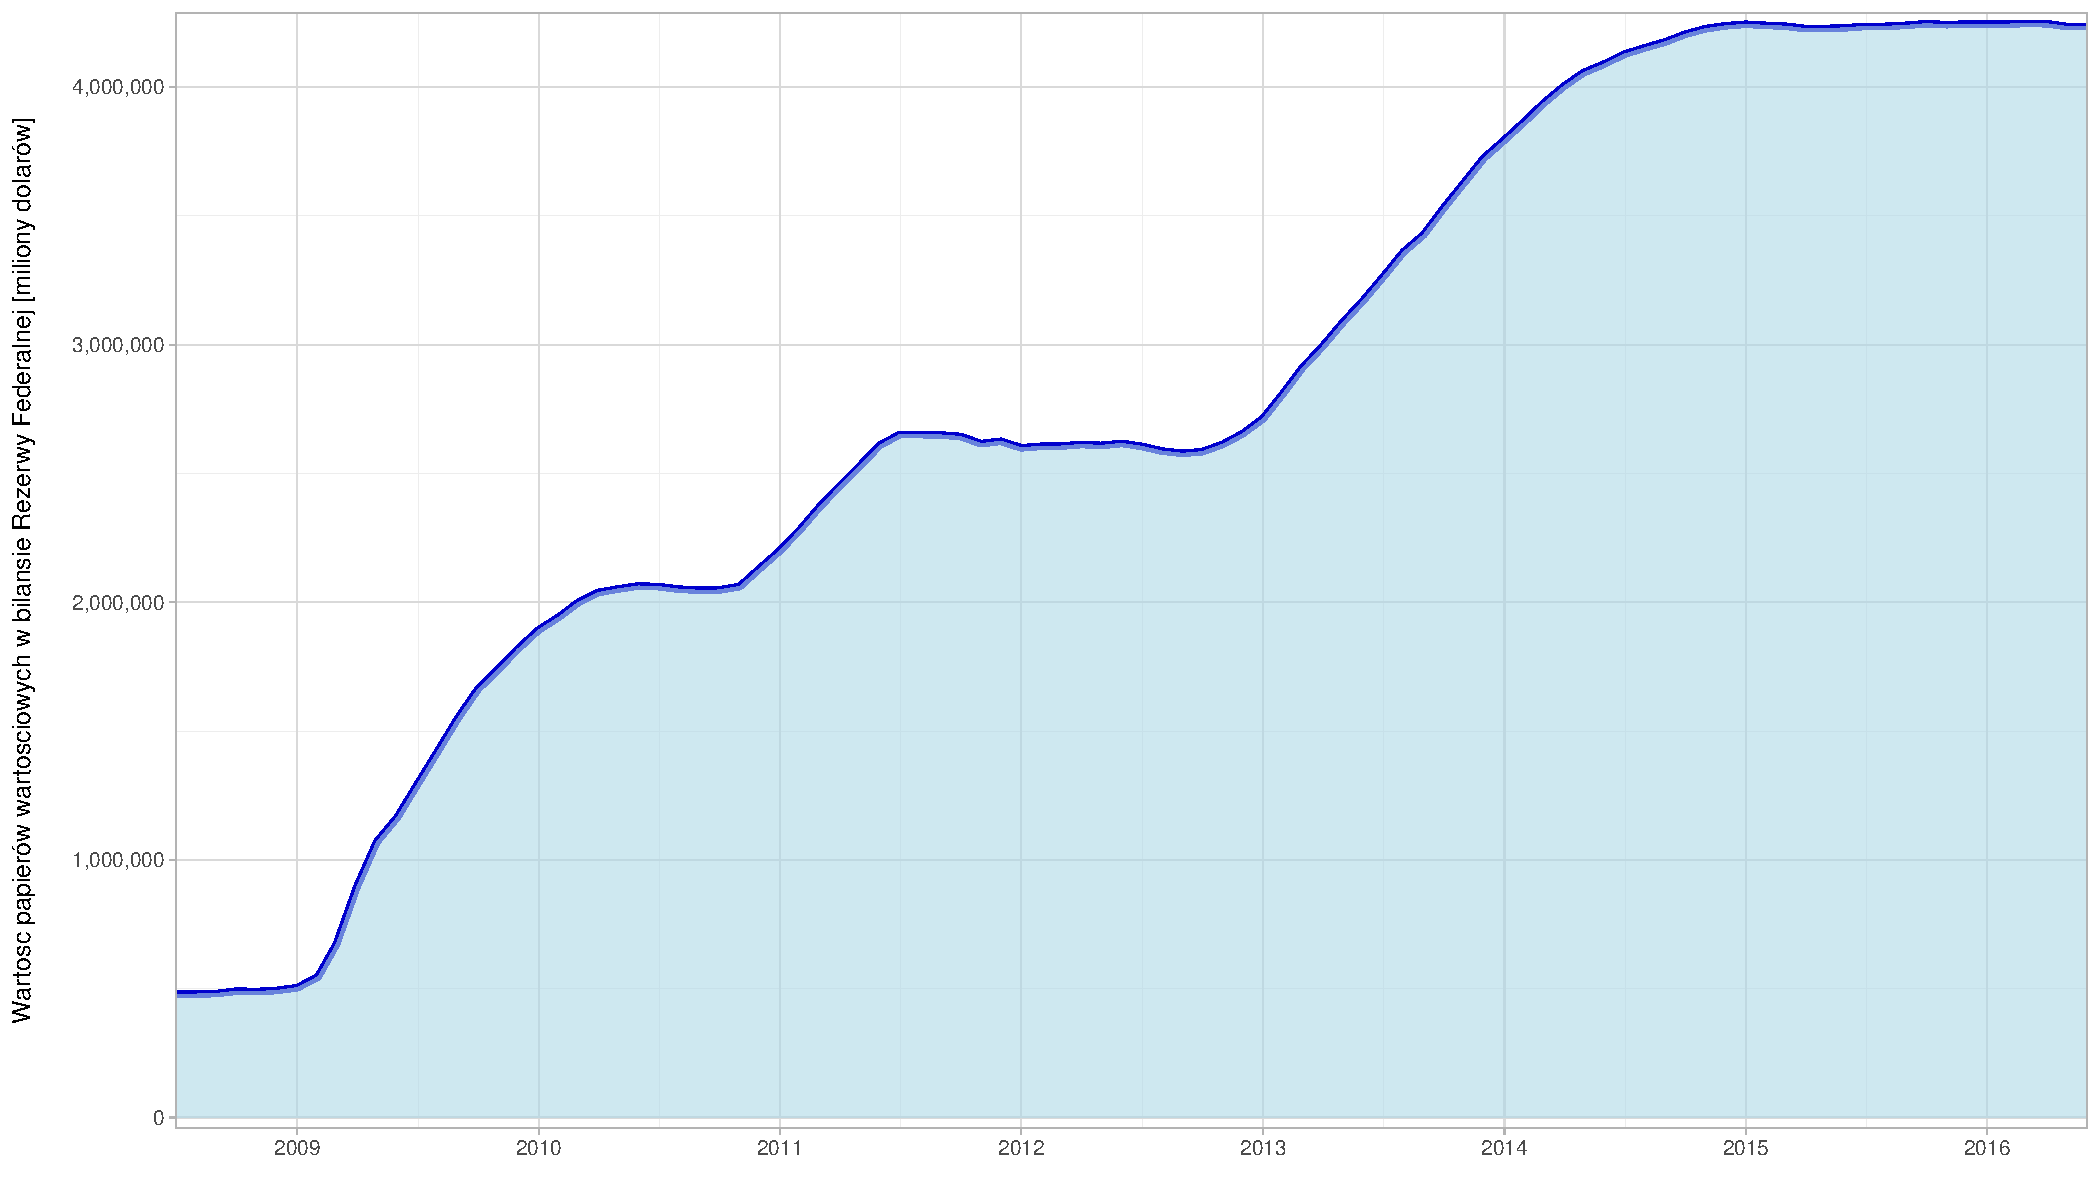
\includegraphics[height=3.5in]{FEDSec}
    \captionsetup{format=hang}
    \caption{Zmienna \textit{FED_Securities} w~okresie 07.2008-06.2016}
\end{centering}
\begin{flushleft}
\hspace{1cm}\textit{\footnotesize{Źródło: Opracowanie własne.}} \\
\end{flushleft}
\vspace{-0.5cm}
\end{figure}

Zmienna \textit{FED_Securities} w~bezpośredni sposób obrazuje skalę i~tempo niekonwencjonalnych działań amerykańskich władz monetarnych na rynkach dłużnych papierów wartościowych (skarbowym i~papierów komercyjnym) w~latach 2008-2016 będąc skumulowaną sumą wartości wszystkich zakupionych przez Rezerwę Federalną papierów wartościowych w~kolejnych odcinkach czasu. \hyperlink{fig13}{Wykres 12} prezentuje sposób w~jaki kształtowała się wyżej wspomniana zmienna w~poszczególnych latach okresu badawczego - widać jej dynamiczny wzrost od końca 2008~roku, z~blisko 500~miliardów dolarów do około 4,5~biliona dolarów, co oznacza przyrost o~niemal 800\% w~6~lat. Tak znacząca kwota pieniędzy (około 25\% \acs{PKB} Stanów Zjednoczonych) wprowadzona przez Rezerwę Federalną na~rynek dłużnych papierów wartościowych w~latach 2008-2016 powinna istotnie wpłynąć na ten segment amerykańskiej gospodarki, ale również nie powinna mieć neutralnego wpływu na pozostałe jej segmenty reprezentowane przez zmienne wykorzystane w~finalnym modelu wektorowej autoregresji. Aby określić czy ten wpływ był statystycznie istotny postanowiono zbadać czy zmienna \textit{FED_Securities} jest przyczyną w~sensie Grangera pozostałych zmiennych. Oznacza to zbadanie, czy przeszłe wartości zmiennej reprezentującej wartość papierów wartościowych w~bilansie Rezerwy Federalnej są w~stanie poprawić jakość prognoz pozostałych zmiennych zawartych w~modelu. W~literaturze często stosuje się również tak zwaną przyczynowość natychmiastową (ang. \textit{instantaneous causality}), która stanowi rozszerzenie przyczynowości w~sensie Grangera o~bieżące wartości badanej zmiennej. Do zbadania czy zmienna \textit{FED_Security} mogła spowodować istotne zmiany pozostałych zmiennych wykorzystanych w~analizowanym w~tym rozdziale modelu postanowiono skorzystać z~obu tych przyczynowości. Do zbadania przyczynowości w~sensie Grangera, jak i~przyczynowości natychmiastowej zastosowano odpowiednie testy statystyczne, których wyniki zaprezentowano w~\hyperlink{tab6}{tabeli nr 7}. 

\hypertarget{tab6}{}
\begin{table}[!ht]
\rowcolors{2}{lightgray}{white}
\captionsetup{format=hang, position=top}
\caption{Wyniki testów na przyczynowość w~sensie Grangera oraz na przyczynowość natychmiastową zmiennej \textit{FED_Securities} w~finalnym modelu VAR}
\begin{tabular}{
M{4.5cm}
M{4cm}
S[table-format=2.3]
S[table-format=1.3]
}
\toprule
\textbf{Nazwa testu} & \textbf{Hipoteza zerowa} & \textbf{St. testowa} & \textbf{P-value} \\
\midrule
Przycz. Granger    &  Brak przyczynowości &   3,862  & 0,000\\
Przycz. natychmiastowa &  Brak przyczynowości &  19,177  & 0.014\\
\bottomrule
\end{tabular}
\begin{flushleft}
\hspace{1cm}\textit{\footnotesize{Źródło: Opracowanie własne.}} \\
\end{flushleft}
\vspace{-0.5cm}
\end{table} 

Wyniki obu testów wskazują, iż na 5\%-owym poziomie istotności należy odrzucić hipotezę zerową o~braku przyczynowości - zmienna \textit{FED_Securities} jest przyczyną zarówno w~sensie Grangera, jak i~natychmiastową, pozostałych zmiennych z~finalnego modelu \acs{VAR}. Oznacza to, iż zasadne jest badanie wpływu niekonwencjonalnej polityki monetarnej Rezerwy Federalnej na zmienne reprezentujące wybrane segmenty amerykańskiej gospodarki.

\subsection*{\normalsize{Analiza funkcji odpowiedzi na impuls finalnego modelu VAR}}

Pierwszym etapem badania relacji pomiędzy zmiennymi w~finalnym modelu \acs{VAR} jest analiza funkcji odpowiedzi na impuls (\acs{IRF}). W~związku z~tym, iż niniejsza praca skupia się na wpływie niekonwencjonalnej polityki pieniężnej na amerykańską gospodarkę, analiza funkcji \acs{IRF} dotyczyć będzie szoku zmiennej \textit{FED_Securities}, zdefiniowanego jako jej jeden błąd standardowy z~badanej próby z~lat 2008-2016 (około 120~miliardów dolarów) oraz jej wpływie na pozostałe zmienne modelu: \textit{PCE}, \textit{Stopa_bez}, \textit{PKB_realne}, \textit{SP500}, \textit{Yield1YGov}, \textit{Yield10Gov}, \textit{UnempDur}, \textit{EURUSD}. \hyperlink{fig14}{Wykres 13}~prezentuje funkcje odpowiedzi na impuls zmiennych finalnego modelu \acs{VAR} oraz odpowiednie 95\%-owe przedziały ufności tych funkcji wyznaczone za pomocą metody \textit{bootstrap} \footnote{Uzyskane przedziały ufności okazały się stosunkowo szerokie. Przedziały podobnej szerokości obserwuje się również w~literaturze dotyczącej niekonwencjonalnej polityki monetarnej i~jest to związane z~niską liczbą stopni swobody wynikającą z~małej liczby obserwacji w~odniesieniu do liczby zmiennych i~ich opóźnień w~modelu}. Ze względu na miesięczną częstotliwość danych zdecydowano się na analizę funkcji \acs{IRF} w~skumulowanej perspektywie rocznej.

\vspace{0.25cm}
\hypertarget{fig14}{}
\begin{figure}[h]
\begin{centering}
  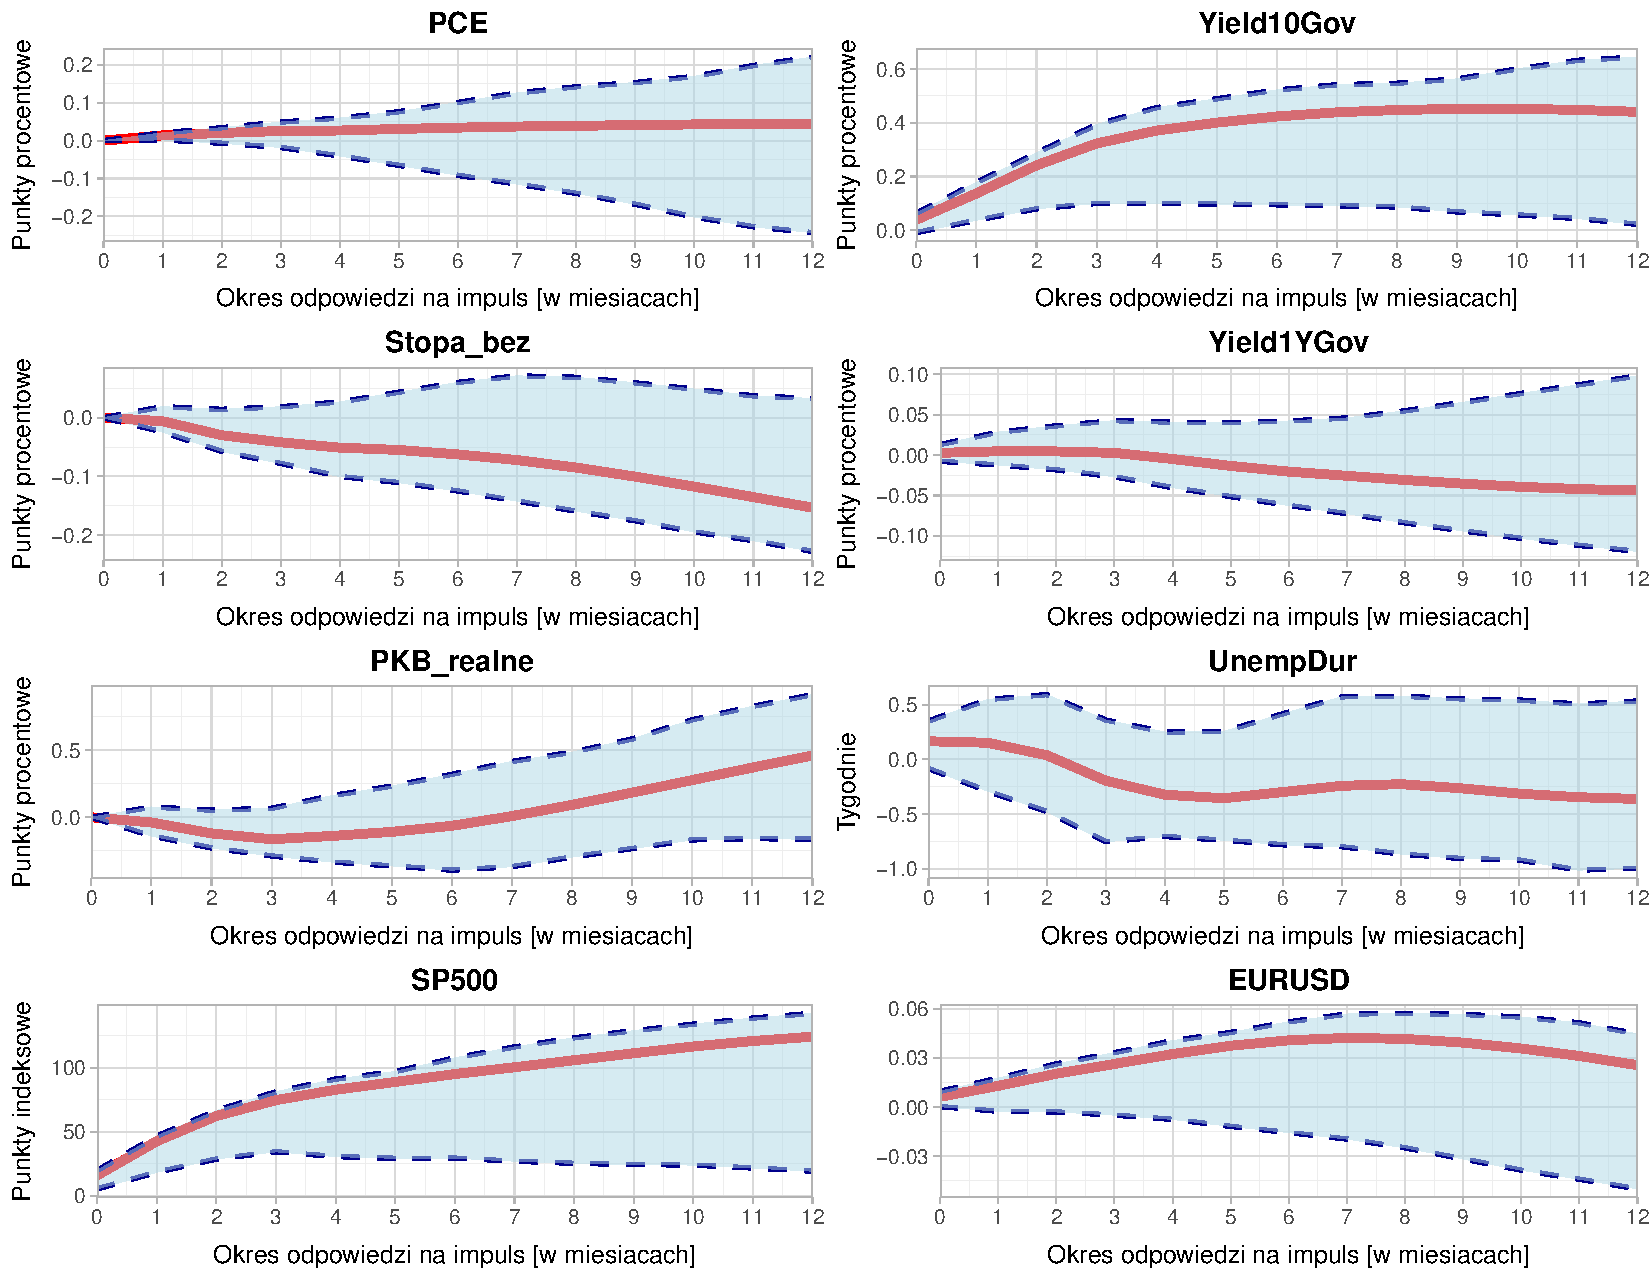
\includegraphics[height=4.8in]{IRFs}
    \captionsetup{format=hang}
    \caption{Funkcje odpowiedzi zmiennych z~modelu VAR na impuls niekonwencjonalnej polityki pieniężnej Rezerwy Federalnej oraz 95\% przedziały ufności tych funkcji.}
\end{centering}
\begin{flushleft}
\vspace{-0.3cm}
\hspace{1cm}\textit{\footnotesize{Źródło: Opracowanie własne.}} \\
\end{flushleft}
\vspace{-0.5cm}
\end{figure}

Wykres reakcji zmiennej \textit{PCE} wskazuje, iż nieoczekiwany wzrost wartości dłużnych instrumentów finansowych skupowanych przez Rezerwę Federalną o~około 120~miliardów dolarów (6\% \acs{PKB} Stanów Zjednoczonych) mógł wpłynąć w~rocznej perspektywie na wzrost wskaźnika cen o~0,05~punktu procentowego (3\% średniej wartości zmiennej w~latach 2008-2016). Kierunek i~skala zmiany zmiennej \textit{PCE} wydaje się wskazywać, iż niekonwencjonalna polityka monetarna Rezerwy Federalnej nie wywarła wielkiego wpływu na poziom cen w~amerykańskiej gospodarce. Nie mniej jednak jest obserwacje te są zgodne z~wnioskami badawczymi odnotowywanymi w~literaturze, gdzie reakcja poziomu cen na niekonwencjonalną politykę monetarną kształtowała się na poziomie od 0,02 p.p. do 0,15 p.p.

Wykres reakcji zmiennej \textit{Yield10Gov} wskazuje, iż innowacja w~polityce monetarnej Rezerwy Federalnej polegająca na zastosowaniu niekonwencjonalnej polityki pieniężnej w~skali około 120~miliardów dolarów mogła doprowadzić do wzrostu dziesięcioletniej krzywej dochodowości o~około 45~punktów bazowych (17\% średniej wartości zmiennej \textit{Yield10Gov}). Takie zachowanie analizowanej zmiennej wydaje się sprzeczne z~oczekiwaniami szefów amerykańskich władz monetarnych - jednym z~ich głównych celów było obniżenie długoterminowych rentowności amerykańskich obligacji skarbowych, tymczasem model \acs{VAR} wskazuje, iż nie tylko nie zrealizowano tego celu, ale efekty ich działań mogły przynieść skutek odwrotny, przynajmniej w~tym fragmencie krzywej dochodowości. Obserwacje te pozostają jednak w~zgodzie z~wnioskami wypływającymi z~pierwszej części rozdziału, gdzie ogłaszanie kolejnych niekonwencjonalnych programów (poza pierwszym z~nich) prowadziło w~krótkoterminowej perspektywie do wzrostu krzywej dochodowości. Jak widać efekt wzrostu rentowności amerykańskich obligacji skarbowych na skutek niekonwencjonalnych działań Rezerwy Federalnej utrzymał się w~okresie dłuższym niż kilka miesięcy i~reakcja ta była silniejsza niż obserwowana w~krótszym terminie. Mogłoby to potwierdzać hipotezę o~odpływie kapitału z rynków dłużnych długoterminowych papierów wartościowych jako reakcji inwestorów na ogłaszanie kolejnych niekonwencjonalnych programów. Obserwacje te jednak, jak już wcześniej wspominano, stoją w~sprzeczności z~literaturą badawczą, gdzie nadzwyczajne działania Rezerwy Federalnej miały prowadzić do statystycznie istotnej obniżki rentowności amerykańskich obligacji skarbowych w skali od 0,05 do 0,5 punktu procentowego. Reakcja krótkiego końca krzywej dochodowości na poziomie około -5~punktów bazowych (14\% średniej rentowności rocznych obligacji) badana przy użyciu zmiennej \textit{Yield1YGov} każe z~kolei przypuszczać, iż nie cała krzywa dochodowości reagowała tak samo na niekonwencjonalną politykę monetarną - bliższy koniec krzywej wydaje się bardziej wrażliwy na działania Rezerwy Federalnej reagując zgodnie z~jej intencjami oraz z~badaniami przestawionymi w~literaturze.

Funkcja odpowiedzi na impuls zmiennej \textit{PKB_realne} pokazuje, że szok w~polityce monetarnej amerykańskich władz monetarnych w~pierwszych sześciu miesiącach mógł wpłynąć na osłabienie wzrostu gospodarczego by w~kolejnych 6~miesiącach doprowadzić do jego umocnienia notując ostatecznie w~rocznej perspektywie pozytywną zmianę na poziomie blisko 50~punktów bazowych (39\% średniej wartości zmiennej w~latach 2008-2016). Taki efekt byłby zbieżny z~oczekiwaniami Rezerwy Federalnej (oraz z~literaturą badawczą), gdyż oznacza realny i~istotny wpływ jej działań na amerykańską gospodarkę, pomimo odwrotnego od zamierzeń wpływu na długoterminową krzywą dochodowości.

Ostatnią istotną funkcją reakcji na szok w~polityce monetarnej jest \acs{IRF} zmiennej \textit{SP500}, gdzie w~perspektywie rocznej umieszczenie przez Rezerwę Federalną 120~miliardów dolarów na rynku dłużnych papierów skarbowych mogło spowodować wzrost indeksu S\&P500 o~około 150 punktów bazowych, czyli ponad 10\% średniej wartości indeksu w~latach 2008-2016. Wiedząc, iż średnia kapitalizacja wszystkich spółek należących do indeksu S\&P500 w~latach 2008-2016 wynosiła około 15~bilionów dolarów, można wyliczyć, iż wzrost indeksu o~10\% oznacza wzrost wycen spółek o~około 1,5~biliona dolarów. Rynek akcji mógłby być więc jednym z~tych rynków, na który odpłynął kapitał z~rynku amerykańskich obligacji skarbowych. Podobne wnioski tylko o~mniejszej oszacowanej skali (0,2-1\% pozytywnego wpływu \acs{MNK} na poziom cen) można odnaleźć w~przedstawionej w~drugim rozdziale literaturze badawczej(\cite{chen36}, \cite{bhattarai36}, \cite{swanson37}).

Reakcje stopy bezrobocia, mediany czasu trwania bezrobocia oraz kursu EUR/USD okazały się nieistotne odnosząc skalę ich reakcji na impuls niekonwencjonalnej polityki monetarnej do ich średnich wartości (odpowiednio -2\%, -2,5\% i~2\%). Wygląda więc na to, iż nadzwyczajne działania Rezerwy Federalnej nie wpłynęły istotnie na rynek pracy oraz rynek walutowy, mogły jednak mieć istotny wpływ na zachowanie się rynków dłużnych papierów skarbowych oraz akcji, a~także poziomu produkcji i~cen w~amerykańskiej gospodarce. Obserwacje te dobrze jest jednak potwierdzić analizą funkcji dekompozycji wariancji błędów prognoz.

\subsection*{\normalsize{Analiza dekompozycji wariancji błędów prognoz finalnego modelu VAR}}

Kolejnym etapem badania relacji pomiędzy zmiennymi w~finalnym modelu wektorowej autoregresji jest analiza dekompozycji wariancji błędów prognoz (ang. \textit{Forecast Error Variance Decomposition - FEVD}). Pozwala ona sprawdzić jaka część wariancji zmiennej jest skutkiem jej własnego szoku, a~jaka wynika z~szoku innych zmiennych, ukazując tym samym dynamikę rozchodzenia się szoków po systemie równań modelu \acs{VAR}. Podobnie jak w~przypadku funkcji \acs{IRF} główny nacisk analizy został położony na wpływ szoku zmiennej \textit{FED_Securities} na pozostałe zmienne wykorzystane w~modelu. \hyperlink{fig15}{Wykres 14} prezentuje dekompozycje wariancji błędów prognoz dla wszystkich zmiennych wykorzystanych w~analizowanym modelu  \acs{VAR}. Jak widać zmienna \textit{FED_Securities} istotnie wpływa na wariancję jedynie dwóch zmiennych (wyłączając jej własną wariancję): \textit{SP500} oraz \textit{Yield10Gov}, w~rocznej perspektywie wyjaśniając odpowiednio: 21\% oraz 14\% ich zmienności. W~przypadku pozostałych zmiennych wpływ ten jest marginalny - nie przekracza 7\%. 

\vspace{0.25cm}
\hypertarget{fig15}{}
\begin{figure}[h]
\begin{centering}
  \hspace{-0.55cm}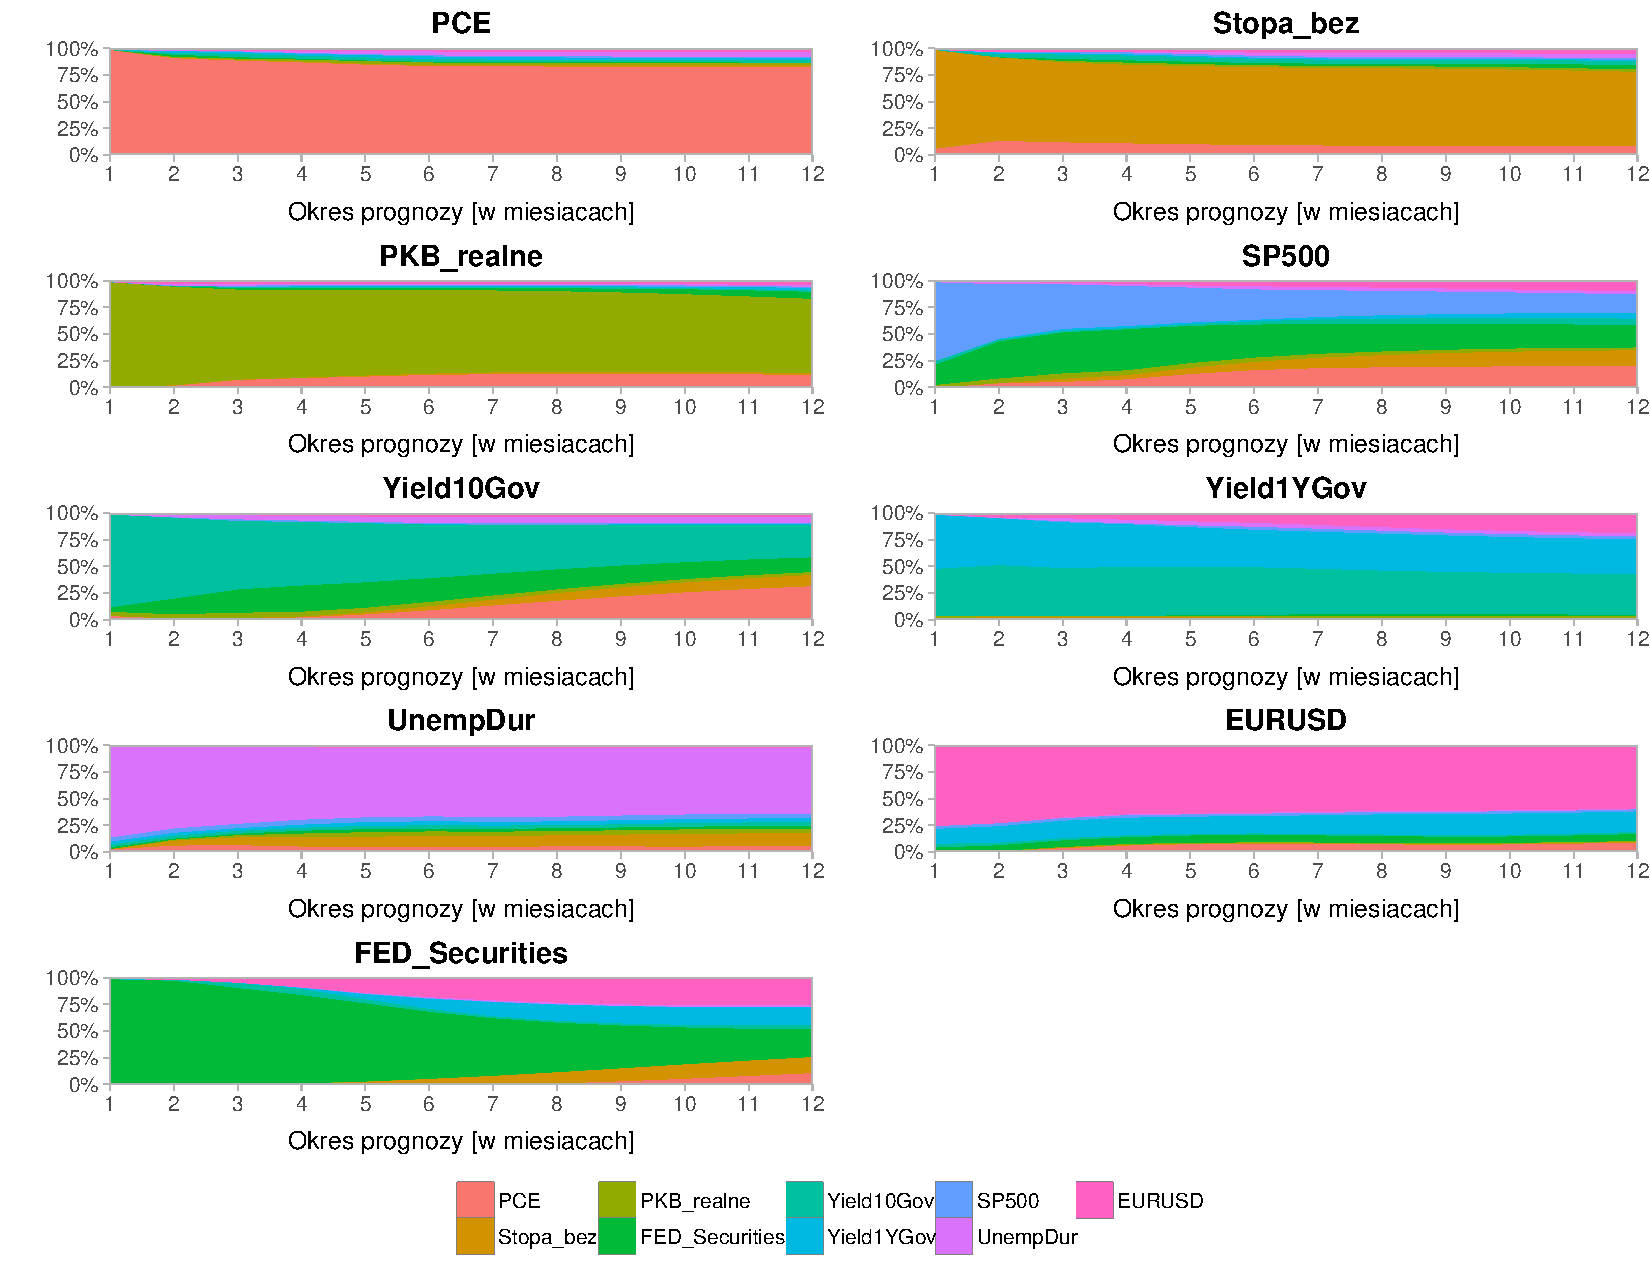
\includegraphics[height=6in, width=6.5in]{FEVDs}
    \captionsetup{format=hang}
    \caption{Dekompozycje wariancji błędów prognoz dla zmiennych z~finalnego modelu VAR}
\end{centering}
\begin{flushleft}
\hspace{1cm}\textit{\footnotesize{Źródło: Opracowanie własne.}} \\
\end{flushleft}
\vspace{-0.5cm}
\end{figure} 

Analizując wykres dekompozycji wariancji indeksu S\&P500 można zaobserwować, iż o~ile w~pierwszym miesiącu na wariancję tej zmiennej wpływa przede wszystkim jej szok własny (74\% zmienności), co jest całkowicie naturalne, to w~perspektywie rocznej najbardziej istotnym czynnikiem kształtującym zmienność tego indeksu jest szok zmiennej reprezentującej wartość papierów dłużnych nabywanych przez Rezerwę Federalną (21\% zmienności przy zaledwie 17\% zmienności wynikającej z~szoku \textit{SP500}). W~przypadku pozostałych analizowanych zmiennych przeważający wpływ w~całym oknie badawczym mają w~przeważającej większości szoki własne tych zmiennych. Takie zachowanie wariancji indeksu S\&P500 może wskazywać na silny wpływ niekonwencjonalnej polityki monetarnej na amerykański rynek akcji w~badanym okresie co wzmacniałoby obserwacje poczynione przy okazji badania funkcji odpowiedzi na impuls. 

Wykres dekompozycji wariancji błędów prognoz dla dziesięcioletnich rentowności amerykańskich obligacji skarbowych wskazuje, iż wpływ szoku niekonwencjonalnej polityki monetarnej na zmienność \textit{Yield10Gov} wynosił od 4\% w~pierwszym miesiącu przez 25\% w~czwartym aż po 14\% w~rocznej perspektywie - konsumując dużą część spadku wpływu zmienności własnej (z~87\% do 31\%). Potwierdza to istotność oddziaływania decyzji amerykańskich władz monetarnych na rynek długoterminowych obligacji skarbowych w~krótkiej i~średniej perspektywie odnotowaną w~poprzednim podrozdziale, a~także przy analizie funkcji odpowiedzi na impuls. Poza wpływem zmiennej \textit{FED_Securities} na \hyperlink{fig15}{wykresie 14} widać również inne istotne powiązania pomiędzy zmiennymi wykorzystanymi w~finalnym modelu wektorowe-autoregresji:
\begin{itemize}
\setlength\itemsep{0.05cm}
\item duży udział szoku na rentowności dziesięcioletnich amerykańskich obligacji skarbowych w~zmienności rentowności obligacji rocznych (od 44\% do 38\%) przy praktycznym braku symetrycznej zależności - co może potwierdzać rolę obligacji dziesięcioletnich jako punktu odniesienia całego rynku obligacji skarbowych,
\item blisko 33\%-owy udział szoku zmiennej \textit{PCE} w~wariancji zmiennej \textit{Yield10Gov} (udział ten jest wyższy nawet od udziału szoku własnego zmiennej 31\%), co może wskazywać na silny wpływ odczytów poziomu cen na kształtowanie się rentowności długoterminowych obligacji,
\item 21\% zmienności S\&P500 zdaje się tłumaczyć szok na wskaźniku cen \textit{PCE} - co wskazywałoby na jego istotność w~procesie decyzyjnym uczestników amerykańskiego rynku akcji,
\item 18\%-owy udział szoku na kursie EUR/USD w~całkowitej wariancji zmiennej \textit{Yield1YGov} przy 20\% relacji odwrotnej, co może być tłumaczone istotnym udziałem podmiotów zagranicznych w~tym fragmencie rynku amerykańskich dłużnych papierów skarbowych,
\item 15\% zmienności S\&P500 zdaje się tłumaczyć szok na wskaźniku bezrobocia \textit{Stopa_bez} - co wskazywałoby na jego istotność w~procesie decyzyjnym uczestników amerykańskiego rynku akcji,
\item 13\% wariancji realnego produktu krajowego brutto tłumaczy zmienność indeksu prywatnych wydatków konsumpcyjnych,
\item około 12\% zmienności średniej długości trwania bezrobocia mogą tłumaczyć szoki na stopie bezrobocia, co wydaje się oczywiste, dziwić może jedynie niska skala wpływu,
\item największy wpływ na wariancję zmiennej \textit{FED_Securities} (poza szokiem jej samej) miały szoki zmiennych: kurs EUR/USD (24\%), rentowność rocznych obligacji skarbowych (17\%), stopa bezrobocia (15\%), roczna zmiana \acs{PKB} realnego (13\%) oraz wskaźnik \acs{PCE} (12\%). Zmienne te pokrywają się z~celami banku centralnego Stanów Zjednoczonych, co nie powinno dziwić w sytuacji, gdy wartość zmiennej \textit{FED_Securities} w~latach 2008-2016 zależała ściśle od decyzji Rezerwy Federalnej. Jednakże kolejność i~istność poszczególnych celów amerykańskich władz monetarnych znacznie się różni się od tej z~dekompozycji wariancji błędów prognoz.
\end{itemize}

Analiza dekompozycji wariancji błędów prognoz potwierdza poprzednie obserwacje dotyczące wpływu niekonwencjonalnej polityki pieniężnej na rynek dłużnych papierów skarbowych oraz rynek akcji. Nie potwierdziły się jednak obserwacje dotyczące wpływu zmiennej \textit{FED_Securities} na poziom produkcji - największy wpływ na wariancje zmiennej \textit{PKB_realne} miały szoki własne tej zmiennej (około 70\% w~rocznej perspektywie). Kolejnym i~zarazem ostatnim etapem badania będzie wygenerowanie prognoz z~finalnego modelu \acs{VAR}, sprawdzenie ich jakości porównując je do wartości rzeczywistych (tzw. \textit{backtesting}) oraz interpretacja rocznych prognoz dla okresu lipiec 2016 - czerwiec 2017.

\subsection*{\normalsize{Analiza prognoz uzyskanych z~finalnego modelu VAR}}

Analizę prognoz uzyskanych z~finalnego modelu wektorowej autoregresji rozpoczęto od przeprowadzenia wstecznych testów jakości prognoz dla lat 2008-2016. W~tym celu dla każdego miesiąca pomiędzy lipcem 2008~a~czerwcem 2016~oszacowano osobny model \acs{VAR}, uzyskując łącznie 96~takich modeli. Starano się przy tym wykorzystywać ośmioletnią próbkę danych dla każdego miesiąca, czego nie udało się osiągnąć dla miesięcy z~lat 2008-2009 ze względu na dostępność danych jedynie od stycznia 2002~roku. Z~tak wyestymowanych 96~modeli wygenerowano następnie roczne prognozy, porównano je z~rzeczywistymi realizacjami zmiennych i~wyliczono dla nich pierwiastki błędów średniokwadratowych. Aby zapewnić porównywalność pomiędzy tymi błędami postanowiono zastosować ich standaryzację - dzieląc je przez ich własną średnią i~otrzymano znormalizowane pierwiastki błędów średniokwadratowych (ang. \textit{Normalized Root-Mean-Square Errors - NRMSE}). Wyliczone miesięczne \acs{NRMSE} dla wszystkich zmiennych zostały zagregowane i~uśrednione do lat (patrz \hyperlink{tab7}{tabela 8}). 

\hypertarget{tab7}{}
\begin{table}[!ht]
\rowcolors{2}{lightgray}{white}
\footnotesize
\captionsetup{format=hang, position=top}
\caption{Błędy NRMSE prognoz finalnego modelu VAR w~latach 2008-2016 (jako \% średniej)}
\begin{tabular}{cccccccccc}
\toprule
\textbf{Year} & \textbf{PCE} & \textbf{\begin{tabular}[c]{@{}c@{}}Stopa\\ bezr.\end{tabular}} & \textbf{\begin{tabular}[c]{@{}c@{}}PKB\\ realne\end{tabular}} & \textbf{\begin{tabular}[c]{@{}c@{}}FED\\ Securities\end{tabular}} & \textbf{\begin{tabular}[c]{@{}c@{}}Yield-\\ 10Gov\end{tabular}} & \textbf{SP500} & \textbf{\begin{tabular}[c]{@{}c@{}}Yield-\\ 1YGov\end{tabular}} & \textbf{\begin{tabular}[c]{@{}c@{}}Unemp-\\ Dur\end{tabular}} & \textbf{EURUSD} \\ \midrule
\textbf{2008} & 56\% & 49\% & 344\%  & 30\%  & 71\%  & 41\%  & 597\%  & 48\% & 89\% \\ 
\textbf{2009} & 68\% & 65\% & 867\% & 60\% & 82\% & 142\% & 225\% & 58\% & 96\% \\
\textbf{2010} & 23\% & 30\% & 326\% & 18\% & 37\% & 16\% & 124\% & 22\% & 18\% \\ 
\textbf{2011} & 23\% & 11\% & 106\% & 24\% & 32\% & 17\% & 129\% & 23\% & 16\% \\ 
\textbf{2012} & 32\% & 12\% & 83\% & 14\% & 20\% & 9\% & 61\% & 21\%  & 11\% \\
\textbf{2013} & 31\% & 6\% & 72\% & 14\% & 33\% & 9\% & 39\% & 21\% & 9\% \\
\textbf{2014} & 23\% & 9\% & 42\% & 15\% & 7\% & 6\% & 35\% & 16\% & 10\% \\ 
\textbf{2015} & 5\% & 4\% & 45\% & 24\% & 17\% & 14\% & 33\% & 12\% & 7\% \\ 
\textbf{2016} & 4\% & 2\% & 47\% & 2\% & 9\% & 6\% & 13\% & 21\% & 4\% \\ 
\textbf{Średnia} & 29\% & 21\% & 214\% & 22\% & 34\% & 29\% & 139\% & 27\% & 29\% \\ 
\bottomrule
\end{tabular}
\begin{flushleft}
\hspace{1cm}\textit{\footnotesize{Źródło: Opracowanie własne.}} \\
\end{flushleft}
\vspace{-0.5cm}
\end{table} 

Analiza \hyperlink{tab7}{tabeli 8}~wskazuje, iż najgorsza jakość prognoz została uzyskana w~2009~roku - był to okres najbardziej gwałtownej zmiany wskaźników gospodarczych, a~najlepsza w~2016~roku, co jest zgodne z~oczekiwaniami, gdyż do tego okresu model był dopasowywany. Jakość prognoz z~roku na rok ulegała poprawie, co pozwala być pozytywnie nastawionym do prognoz na okres z~poza próbki. Większość zmiennych okazała się być prognozowana na dobrym poziomie jakości - średnie błędy \acs{NRMSE} w~96~miesięcznych prognozach nie przekroczyły 30\% dla wszystkich zmiennych poza zmiennymi: \textit{PKB_realne} (214\%) oraz \textit{Yield1YGov} (139\%). Najwyższą jakość prognoz uzyskano z~kolei dla: \textit{FED_Securities} oraz \textit{Stopa_bez}, gdzie w~badaniu dla lat 2008-2016 popełniano błędy na poziomie około 1/5 ich wartości średniej. Jeszcze lepsze wyniki uzyskuje się patrząc na sam 2016~rok, gdzie 2/3 zmiennych jest prognozowana przy błędach nie przekraczający 10\% wartości średniej, a~jedynie \acs{PKB} realne (47\%) wyraźnie negatywnie odstaje od pozostałych wskaźników. W~związku z~tym, iż jakość prognoz modelu wektorowej autoregresji można potraktować jako test dopasowania modelu do danych, takie wyniki dla zmiennej \textit{PKB_realne} skłaniają do osłabienia wniosków wynikających dla tej zmiennej z~analizy funkcji odpowiedzi na impuls i~dekompozycji wariancji błędów prognoz.

\hypertarget{fig16}{}
\begin{figure}[!ht]
\begin{centering}
  \hspace{-0.55cm}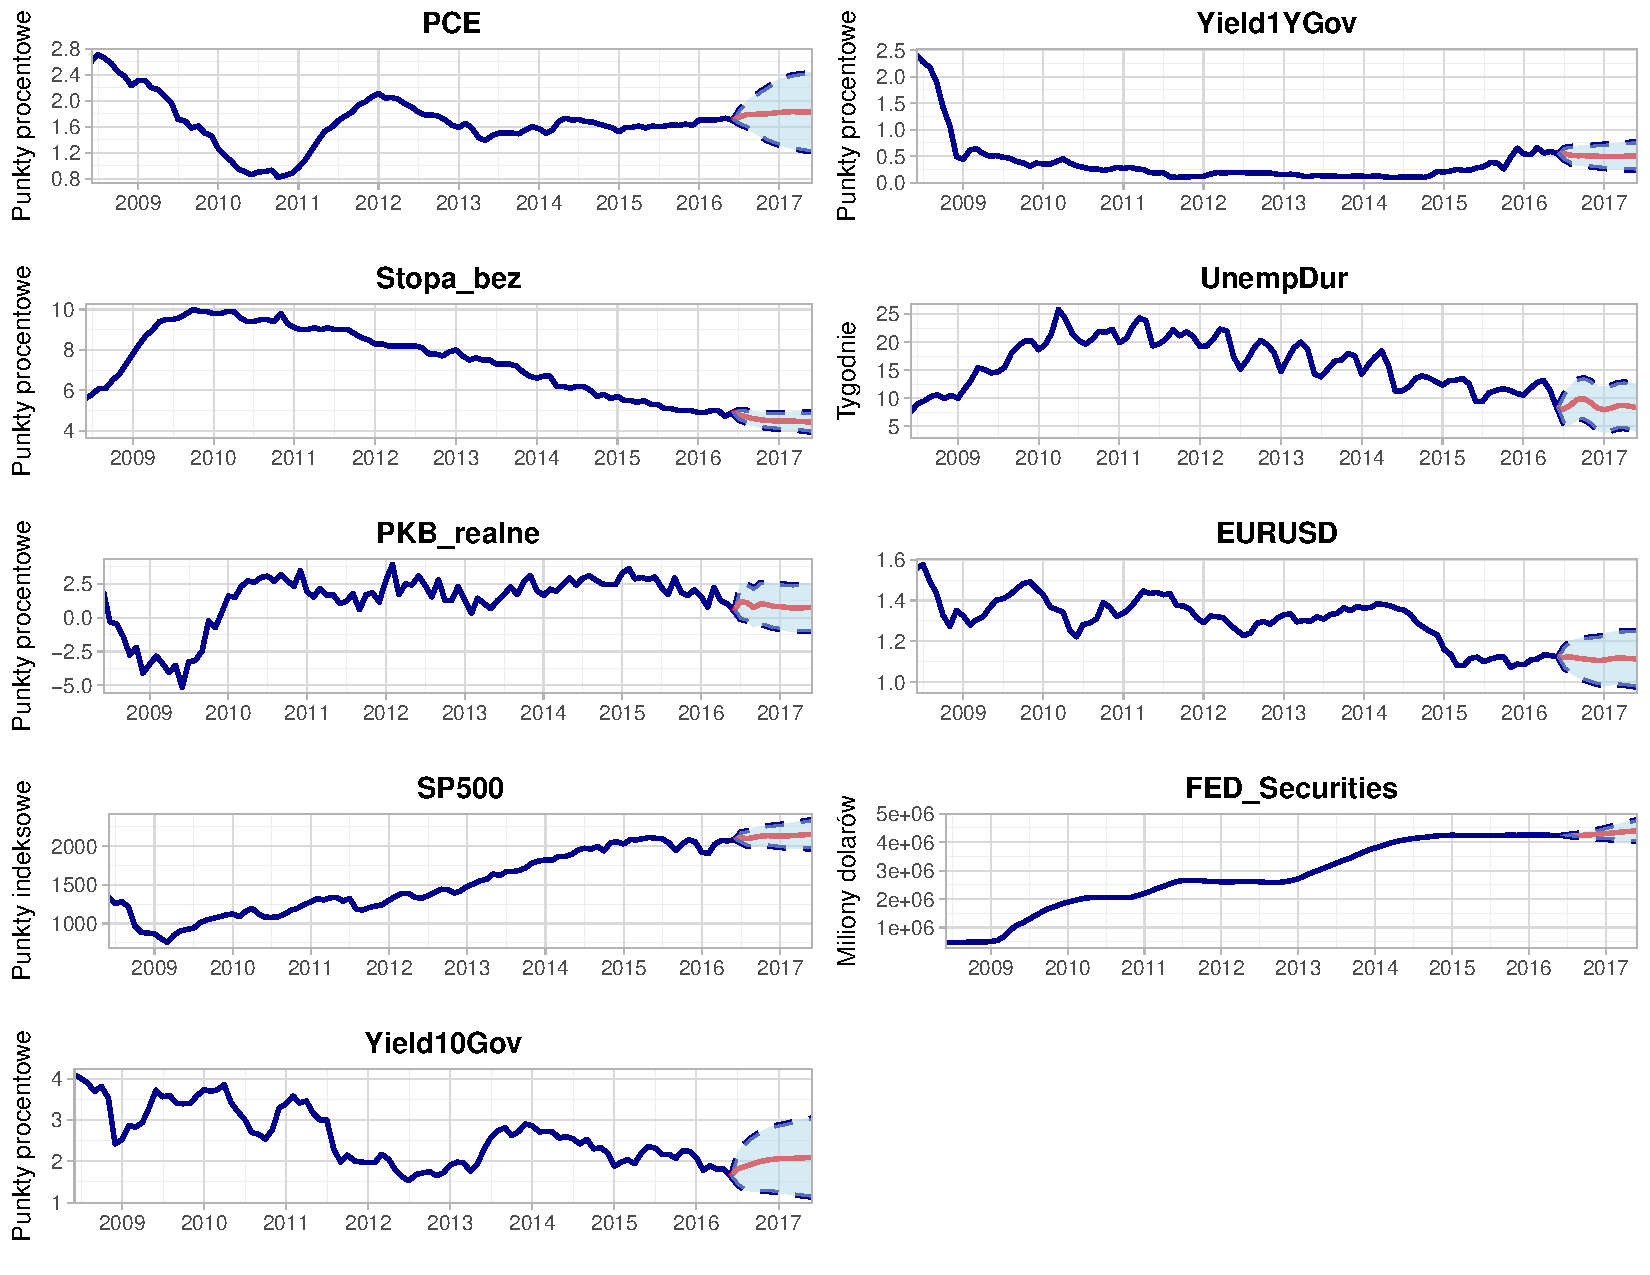
\includegraphics[height=6in, width=6.5in]{Progs}
    \captionsetup{format=hang}
    \caption{Roczne prognozy zmiennych z~finalnego modelu wektorowej autoregresji dla okresu lipiec 2016 - czerwiec 2017 oraz 95\% przedziały ufności tych prognoz}
\end{centering}
\vspace{-0.5cm}
\begin{flushleft}
\hspace{1cm}\textit{\footnotesize{Źródło: Opracowanie własne.}} \\
\end{flushleft}
\vspace{-0.5cm}
\end{figure}

\hyperlink{fig16}{Wykres 15} prezentuje roczne prognozy finalnego modelu wektorowej autoregresji wygenerowane dla wszystkich zmiennych oraz 95\% przedziały ufności tych prognoz wyznaczone za pomocą metody \textit{bootstrap}. Okres prognozy obejmuje 12~miesięcy od lipca 2016~roku do czerwca 2017. Najważniejsze wnioski płynące z~analizy wykresów tych prognoz to:

\vspace{-0.15cm}
\begin{itemize}
\setlength\itemsep{0.05cm}
\item wzrost w~ciągu roku wskaźnika \acs{CPI} z~poziomu 1,6\% do 1,8\% - kontynuacja wzrostu cen w amerykańskiej gospodarce,
\item pogłębienie spadku stopy bezrobocia z~4,9\% w~czerwcu 2016 do 4,6\% w~czerwcu~2017,
\item stabilizacja rocznej zmiany \acs{PKB} realnego na poziomie nie przekraczającym jednego punktu procentowego,
\item powolny wzrost wartości papierów dłużnych w~bilansie Rezerwy Federalnej (200 miliardów dolarów w~ciągu roku),
\item wzrost rentowności dziesięcioletnich amerykańskich obligacji skarbowych od 1,6\% do 2\% oraz stabilizacja rocznych rentowności na poziomie 0,5\%,
\item wzrost wartości indeksu S\&P500 o~ponad 100 punktów indeksowych,
\item stabilizacja mediany czasu trwania bezrobocia w~okolicach~8 tygodni,
\item delikatne umocnienie się dolara w~stosunku do euro - spadek kursu EUR/USD z~poziomu 1,12 do około 1,1. 
\end{itemize}

\noindent Analiza prognoz wygenerowanych z~finalnego modelu wektorowej autoregresji wskazuje w~przypadku większości zmiennych na stabilizację ich wartości w~rocznej perspektywie lub kontynuację dotychczasowych trendów. Najbardziej wartościowymi obserwacjami wydają się prognoza dalszego wzrostu poziomu cen oraz spadku stopy bezrobocia przy stabilizacji rocznej zmiany \acs{PKB} realnego na relatywnie niskim poziomie. Warto pamiętać jednak, iż zmienne \textit{PKB_realne} oraz \textit{Yield1YGov} generowały najwyższe wartości błędów \acs{NRMSE} we wstecznych testach jakości prognoz (kilkukrotnie przekraczające dopuszczalny poziom 30\%), dlatego więc ich prognozy mogą być obarczone dużą skalą niedokładności, związaną z~niewystarczającym dopasowaniem modelu \acs{VAR} dla tych zmiennych. 

\subsection*{\normalsize{Weryfikacja hipotez badawczych}}

W~niniejszym rozdziale zaprezentowano badanie dotyczące wpływu niekonwencjonalnej polityki pieniężnej amerykańskich władz monetarnych na rynek dłużnych papierów skarbowych w~Stanach Zjednoczonych oraz na wskaźniki gospodarcze reprezentujące najistotniejsze segmenty amerykańskiej gospodarki. Główną hipotezą badawczą pracy było stwierdzenie, iż niekonwencjonalna polityka monetarna Rezerwy Federalnej stosowana od 2008~roku zamiast pobudzać do wzrostu realnego \acs{PKB} oraz~zbliżać amerykańską gospodarkę do pełnego zatrudnienia przyczyniła się przede wszystkim do wygenerowania ponadprzeciętnych wzrostów cen akcji notowanych na giełdach w~Stanach Zjednoczonych. Tak sformułowana hipoteza badawcza zakładała nie tylko brak pełnej efektywności kanałów transmisji monetarnej w~przekazywaniu impulsów polityki pieniężnej do realnej gospodarki, ale również strukturalną ułomność kanału kredytowego oraz kanału cen akcji, które pomimo ogromnej stymulacji monetarnej realizowanej poprzez działania banku centralnego, zamierzonej w~przypadku kanału kredytowego oraz niezamierzonej (a~przynajmniej nie deklarowanej) w~przypadku kanału cen akcji, nie przekazały adekwatnie silnego impulsu wzrostowego do amerykańskiej gospodarki. Celem badania zrealizowanego w~tej części pracy było zweryfikowanie przedstawionej hipotezy.

Wyniki badania zaprezentowanego w~pierwszej części omawianego rozdziału wskazują, iż amerykański bank centralny implementując niekonwencjonalne programy polityki monetarnej wpływał istotnie na rynek dłużnych papierów skarbowych w~Stanach Zjednoczonych jednak wpływ ten był zgodny z~intencją banku tylko w~przypadku pierwszego luzowania ilościowego (istotne statystycznie obniżenie rentowności amerykańskich obligacji skarbowych na całej długości krzywej dochodowości). W~przypadku ogłaszania kolejnych niekonwencjonalnych programów oraz w~trakcie ich trwania rentowności amerykańskich obligacji skarbowych reagowały wzrostami lub nie zmieniały istotnie swoich wartości. Wszelkie informacje dotyczące zakończenia tych programów prowadziły natomiast do wzrostów tych rentowności. Aby potwierdzić te obserwacje w~kolejnej części niniejszego rozdziału wyestymowano model wektorowej autoregresji zawierający wskaźniki gospodarcze reprezentujące najistotniejsze segmenty gospodarki Stanów Zjednoczonych.

Wyniki modelu \acs{VAR} przedstawione \hyperlink{podrz32}{w~podrozdziale 3.2.} wskazują na statystycznie istotny, nieobciążony błędami i~silnie oddziałujący wpływ niekonwencjonalnej polityki pieniężnej na tylko dwa segmenty amerykańskiej gospodarki: rynek akcji (reprezentowany przez indeks S\&P500) oraz rynek długoterminowych dłużnych papierów skarbowych (reprezentowany przez rentowność dziesięcioletnich obligacji skarbowych). Analiza tego wpływu na pozostałe segmenty amerykańskiej gospodarki wskazała, iż albo jest on marginalny w~odniesieniu do średniej wartości zmiennej reprezentującej dany segment, albo nie wpływa on istotnie na zmienność danego wskaźnika sektorowego, lub też generuje wysokie wartości błędów prognoz. Może to oznaczać brak istotnego wpływu niekonwencjonalnych działań Rezerwy Federalnej na gospodarkę Stanów Zjednoczonych co wskazywałoby na brak pełnej efektywności kanałów transmisji niekonwencjonalnej polityki monetarnej w~Stanach Zjednoczonych w~latach 2008-2016. 

Analizując wpływ niekonwencjonalnych działań amerykańskich władz monetarnych w~latach 2008-2016 na rynki akcji w~Stanach Zjednoczonych posłużono się funkcją odpowiedzi na impuls polityki monetarnej indeksu S\&P500, która wskazała, iż wzrost wartości zakupionych przez Rezerwę Federalną obligacji o~120~miliardów dolarów mógł spowodować wzrost wartości analizowanego indeksu o~około 150 punktów (10\% jego średniej wartości indeksu w~latach 2008-2016) w~perspektywie rocznej. Z~kolei dekompozycja wariancji błędów prognoz pokazała, iż najistotniejszym czynnikiem (istotniejszym nawet od przeszłych wartości indeksu) kształtującym 20\% zmienności S\&P500 od 2008~roku była niekonwencjonalna polityka Rezerwy Federalnej. Patrząc na wyniki tych analiz oraz wiedząc, iż~10\% wartości analizowanego indeksu odpowiadało w~latach 2008-2016 średnio około 1,5 biliona dolarów można przypuszczać, iż to właśnie rynek akcji wchłonął większość kapitału odpływającego z~rynku dłużnych papierów wartościowych co potwierdziłoby hipotezę główną niniejszej pracy.

Badając wpływ niekonwencjonalnych działań Rezerwy Federalnej w~latach 2008-2016 na rynek długoterminowych dłużnych papierów skarbowych posłużono się funkcją \acs{IRF}, która wskazała, iż wzrost skali niekonwencjonalnej polityki pieniężnej Rezerwy Federalnej o~120~miliardów dolarów mógł doprowadzić do wzrostu rentowności dziesięcioletnich obligacji skarbowych o~około 45~punktów bazowych w~rocznej perspektywie, co ostatecznie potwierdziło wnioski płynące z analizy przeprowadzonej \hyperlink{podrz31}{w~podrozdziale 3.1.} odnośnie odwrotnej od intencji Rezerwy Federalnej reakcji krzywej dochodowości na działania amerykańskiego banku centralnego oraz o~odpływie kapitału z~rynku dłużnych papierów skarbowych. Funkcja dekompozycji wariancji błędów prognoz wskazała z~kolei, iż w~rocznej perspektywie 14\% zmienności rentowności dziesięcioletnich obligacji skarbowych może być wyjaśnione zmiennością skali zakupów dłużnych papierów skarbowych przez Rezerwę Federalną (przy 31\%-owym poziomie wyjaśniania zmiennością własną). Nie jest to oczywiście tak istotny wynik jak w~przypadku indeksu S\&P500 ale pokazuje równie silny wpływ amerykańskich władz monetarnych na ten segment gospodarki Stanów Zjednoczonych.

Porównując uzyskane wyniki z~wynikami przedstawionymi w~artykułach badawczych omówionych w~drugim rozdziale można stwierdzić, iż zgadzają się one ze sobą jedynie częściowo. W~obu z~nich podkreślony zostaje wpływ niekonwencjonalnej polityki monetarnej na rynek akcji w~Stanach Zjednoczonych, jednak oszacowany w~niniejszej pracy wpływ okazał się silniejszy niż ten przedstawiony w~literaturze badawczej. Z~kolei wpływ niekonwencjonalnych działań Rezerwy Federalnej na kształt krzywej dochodowości oszacowany w~niniejszej pracy zdecydowanie różni się od tego przedstawionego w~artykułach badawczych. Autorzy części omówionych w~drugim rozdziale badań przekonują, iż rentowności długoterminowych amerykańskich obligacji skarbowych spadły na skutek niekonwencjonalnej polityki monetarnej prowadzonej przez amerykańskie władze monetarne, w~bieżącej pracy oszacowano, iż zachowanie tych rentowności było całkowicie odwrotne (istotny wzrost rentowności obligacji skarbowych na skutek \acs{NPM}) - wyłączając okres pierwszego luzowania ilościowego.

Wyniki zaprezentowanego w~niniejszym rozdziale badania wskazują na konieczność potwierdzenia głównej hipotezy badawczej niniejszej pracy w~zakresie zaledwie połowicznym - niekonwencjonalna polityka monetarna wpłynęła statystycznie istotnie na wygenerowanie ponadprzeciętnych wzrostów na amerykańskich rynkach akcji. Wpływ nadzwyczajnych działań Rezerwy Federalnej na gospodarkę Stanów Zjednoczonych nie jest tak jednoznaczny. Z~jednej strony oszacowany model \acs{VAR} nie ukazał istotnego wpływu \acs{NPM} na takie zmienne jak stopa bezrobocia, \acs{PCE}, kurs walutowy czy długość trwania bezrobocia, z~drugiej strony istotny wynik dotyczący \acs{PKB} realnego może okazać się obarczony błędami ze względu na słabe dopasowanie modelu. Wygląda więc na to, iż zweryfikowanie tej części hipotezy badawczej wymaga przeprowadzenia dodatkowych badań.
% Zakończenie
%****************************ZAKOŃCZENIE*******************************
\newpage
\chapter*{Zakończenie}
 \addcontentsline{toc}{chapter}{Zakończenie}
 
Niniejsza praca podejmowała problematykę niekonwencjonalnej polityki monetarnej stosowanej przez banki centralne w~sytuacji, gdy konwencjonalne narzędzia przestały przynosić spodziewane efekty. Praca ta skupiała się na zdefiniowaniu najważniejszych założeń \acs{NPM}, opisie zastosowania jej podstawowych instrumentów oraz kanałów jej transmisji. Celem pracy było zbadanie skuteczności tego rodzaju polityki monetarnej w~pobudzaniu wzrostu gospodarczego na przykładzie Stanów Zjednoczonych. Przyjęta na początku pracy hipoteza badawcza zakładała, iż niekonwencjonalna polityka monetarna Rezerwy Federalnej stosowana od 2008~roku zamiast pobudzać do wzrostu realnego \acs{PKB} oraz~zbliżać amerykańską gospodarkę do pełnego zatrudnienia przyczyniła się przede wszystkim do wygenerowania ponadprzeciętnych wzrostów cen akcji notowanych na giełdach w~Stanach Zjednoczonych.

Pierwszy rozdział przedstawiał podstawy teoretyczne niekonwencjonalnej polityki monetarnej od jej najważniejszych założeń, przez jej najpopularniejsze narzędzia na kanałach jej transmisji do realnej gospodarki kończąc. Celem tego rozdziału było zbudowanie fundamentów teoretycznych umożliwiających analizę dalszych części pracy. Drugi rozdział stanowił przegląd wybranych badań z~zakresu niekonwencjonalnej polityki monetarnej prowadzonej przez Rezerwę Federalną w~latach 2008-2016. Wnioski uzyskane w~tym rozdziale z~analizy literatury badawczej posłużyły jako punkt wyjścia do właściwego zdefiniowania modelu badawczego oraz stanowiły punkt odniesienia w~stosunku do dalszych analiz. Rozdział trzeci poświęcony został zdefiniowaniu modeli badawczych oraz analizie wpływu szoków niekonwencjonalnej polityki pieniężnej na kształt krzywej dochodowości amerykańskich obligacji skarbowych oraz na pozostałe wskaźniki gospodarcze. W~rozdziale tym udało się wykazać statystycznie istotny wpływ szoku \acs{NPM} w~skali 120 miliardów dolarów na: wzrost rentowności długoterminowych obligacji skarbowych Stanów Zjednoczonych o~około 45~punktów bazowych oraz wzrost indeksu S\&P500 o~ponad 150~punktów indeksowych.

Hipoteza badawcza zawarta we wstępie niniejszej pracy została potwierdzona jedynie połowicznie - udało się wykazać statystycznie istotny wpływ niekonwencjonalnej polityki monetarnej na wygenerowanie ponadprzeciętnych wzrostów cen akcji notowanych na giełdach w~Stanach Zjednoczonych. Drugiej części hipotezy badawczej nie udało się ani potwierdzić, ani odrzucić - wpływ nadzwyczajnych działań amerykańskich władz monetarnych po 2008~roku na gospodarkę Stanów Zjednoczonych okazał się niejednoznaczny. Cześć wskaźników gospodarczych wykazała drobne reakcje na szoki niekonwencjonalnej polityki monetarnej - skala tych reakcji nie była znacząca z~wyjątkiem PKB realnego, gdzie reakcją na szok \acs{NPM} był wzrost o~50 punktów bazowych, jednak dalsze analizy pokazały, iż reakcja ta może być obarczona błędem słabego dopasowania modelu.

Zagadnienie niekonwencjonalnej polityki pieniężnej banków centralnych i~jej wpływu na gospodarkę oraz rynki finansowe, co oczywiste, nie zostało w~niniejszej pracy wyczerpane. Otwarta pozostaje kwestia wpływu \acs{NPM} na amerykańską gospodarkę, co daje pole do dalszych prac badawczych, w~sytuacji gdy dostępne będą dane z~dłuższego horyzontu badawczego, zawierające w~szczególności okres wychodzenie amerykańskiej gospodarki z~niekonwencjonalnej polityki monetarnej. Warty dokładniejszego zbadania jest też wpływ \acs{NPM} na krzywą dochodowości amerykańskich obligacji skarbowych, gdyż wyniki uzyskane w~niniejszej pracy w~tej kwestii wydają się stać w~sprzeczności z~wynikami pojawiającymi się w~dużej części literatury badawczej. Mimo to wydaje się, iż uprawnione jest stwierdzenie, że zaprezentowane w~niniejszej pracy badanie wnosi nowe, istotne obserwacje do literatury dotyczącej niekonwencjonalnej polityki monetarnej.

%============================================================

%===========================BIBLIOGRAFIA=====================

\begin{thebibliography}{7}
 \addcontentsline{toc}{chapter}{Bibliografia}
\bibitem{bagus23}
	Bagus P., Howden D. [2009], 
	\emph{Qualitative Easing in support of a~tumbling financial system: a~look at the eurosystem's recent balance sheet policies}, Economic Affairs, Vol. 29, Issue 4, 60-65.	 
\bibitem{bernanke11}
	Bernanke B. S. [2010],
	\emph{The Economic Outlook and Monetary Policy}, \url{https://www.federalreserve.gov/newsevents/speech/bernanke20100827a.pdf},
	 System Rezerwy Federalnej, Jackson Hole, dostęp: styczeń 2017.
\bibitem{bernanke18}
	Bernanke B. S. [2013],
	\emph{Transcript of Chairman Bernanke’s Press Conference}, \url{http://www.federalreserve.gov/mediacenter/files/FOMCpresconf20130619.pdf},
	 System Rezerwy Federalnej, Waszyngton, dostęp: styczeń 2017.
\bibitem{bhattarai36}
	Bhattarai S., Chatterjee A. , Park W. Y. [2015], 
\emph{Effects of US Quantitative Easing on Emerging Market Economies},  \url{http://www.dallasfed.org/assets/documents/institute/wpapers/2015/0255.pdf}, Bank Rezerwy Federalnej w~Dallas, Dallas, dostęp: styczeń 2017.
\bibitem{chadha03} 
	Chadha J., Waters A. [2011],
	\emph{Quantitative Easing and Bond Yields: Results from a Macro-Finance Yield Curve}, \url{https://editorialexpress.com/cgi-bin/conference/download.cgi?db_name=CEF2011&paper_id=307}, Kent, dostęp: styczeń 2017.
\bibitem{chen36} 
Chen Q., Filardo A., He D., Zhu F. [2016],
\emph{Financial crisis, US unconventional monetary policy and international spillovers}, Journal of International Money and Finance, Vol.67, s.62-81.
\bibitem{christensen04}
	Christensen J., Rudebusch G. [2012],
	\emph{The Response of Interest Rates to U.S. and U.K. Quantitative Easing}, \url{http://www.frbsf.org/economic-research/files/wp12-06bk.pdf}, Bank Rezerwy Federalnej San Francisco, San Francisco, dostęp: styczeń 2017.	
\bibitem{christensen21}
Christensen J., Krogstrup S. [2016], 
\emph{Unconventional Monetary Policy: Lessons for the Transmission of Quantitative Easing}, \url{http://www.frbsf.org/economic-research/files/wp2014-18.pdf}, Bank Rezerwy Federalnej San Francisco, San Francisco, dostęp: styczeń 2017.
\bibitem{davtyan35}
Davtyan K. [2016], 
\emph{The Distributive Effects of Conventional and Unconventional Monetary Policies}, \url{http://www.ub.edu/irea/working_papers/2016/201606.pdf}, Instytut Badań nad Stosowaną Regionalną i~Publiczną Ekonomią, Barcelona, dostęp: styczeń 2017.	
\bibitem{ebc22}
Europejski Bank Centralny [2004], \textit{The Longer Term Refinancing Operations of the EBC}, \url{http://www.ecb.int/pub/pdf/scpwps/ecbwp359.pdf}, Frankfurt, dostęp: styczeń 2017.
\bibitem{gagnon34}
Gagnon J., Raskin M., Remache J., Sack B. [2011],
	\emph{The Financial Market Effects of the Federal Reserve's Large-Scale Asset Purchases}, International Journal of Central Banking, Vol. 7, 3-43. 
\bibitem{gambacorta35}
Gambacorta L., Hofmann B., Peersman G. [2014],
	\emph{The Effectiveness of Unconventional Monetary Policy at the Zero Lower Bound: A Cross-Country Analysis}, Journal of Money, Credit and Banking, Vol. 46, 615-642. 
\bibitem{kagraoki05}
Kagraoki Y., Moussa Z. [2010],
	\emph{Quantitative Easing, Credibility and the Time-Varying Dynamics of the Term Structure of Interest rate in Japan},
	Journal of International Financial Markets, Institutions and Money, Vol. 25, 181–201.
\bibitem{megg23}	
Meggyesi P. [2010],
 	\emph{Reflections on negative interest rates in
Switzerland}, \url{https://snbchf.com/wp-content/uploads/2012/10/JP-Morgan-on-Negative-Interests.pdf}, J.P. Morgan, Nowy York, dostęp: styczeń 2017.		
\bibitem{nelson01}
 	Nelson C. R., Siegel A.F. [1987], 
  	\emph{Parsimonious Modeling  of  Yield  Curves}, 
  	Journal  of Business, Volume 60, 473-489.
\bibitem{Fed09}
 	System Rezerwy Federalnej [2008],
 	\emph{Notatka prasowa z dnia 25. listopada 2008 roku},
 	\url{http://www.federalreserve.gov/newsevents/press/monetary/20081125b.htm}, Waszyngton, dostęp: styczeń 2017.	
\bibitem{Fed10}
 	System Rezerwy Federalnej [2009],
 	\emph{Notatka prasowa z dnia 18. marca 2009 roku},
 	\url{http://www.federalreserve.gov/newsevents/press/monetary/20090318a.htm}, Waszyngton, dostęp: styczeń 2017.	
\bibitem{Fed12}
 	System Rezerwy Federalnej [2010],
 	\emph{Notatka prasowa z dnia 3. listopada 2010 roku},
 	\url{http://www.federalreserve.gov/newsevents/press/monetary/20101103a.htm}, Waszyngton, dostęp: styczeń 2017.	
\bibitem{Fed13}
 	System Rezerwy Federalnej [2011],
 	\emph{Notatka prasowa z dnia 21. września 2011 roku},
 	\url{http://www.federalreserve.gov/newsevents/press/monetary/20110921a.htm}, Waszyngton, dostęp: styczeń 2017.
\bibitem{Fed14}
 	System Rezerwy Federalnej [2012],
 	\emph{Notatka prasowa z dnia 13. września 2012 roku},
 	\url{http://www.federalreserve.gov/newsevents/press/monetary/20120913a.htm}, Waszyngton, dostęp: styczeń 2017.
\bibitem{Fed15}
 	System Rezerwy Federalnej [2012],
 	\emph{Notatka prasowa z dnia 12. grudnia 2012 roku},
 	\url{http://www.federalreserve.gov/newsevents/press/monetary/20121212a.htm}, Waszyngton, dostęp: styczeń 2017.
\bibitem{Fed16}
 	System Rezerwy Federalnej [2013],
 	\emph{Notatka prasowa z dnia 18. grudnia 2013 roku},
 	\url{http://www.federalreserve.gov/newsevents/press/monetary/20131218a.htm}, Waszyngton, dostęp: styczeń 2017.
\bibitem{Fed17}
 	System Rezerwy Federalnej [2014],
 	\emph{Notatka prasowa z dnia 29. października 2014 roku},
 	\url{http://www.federalreserve.gov/newsevents/press/monetary/20141029a.htm}, Waszyngton, dostęp: styczeń 2017.
\bibitem{svensson02}
	Svensson L.O. [1994],
	\emph{Estimating Forward Interest Rates with the Extended Nelson and Siegel Method},
	Sveriges Riksbank Quarterly Review 1995:3, 13-26. 
\bibitem{swanson37}
	Swanson E. T. [2015],
	\emph{Measuring the Effects of Unconventional Monetary Policy on Asset Prices}, \url{http://www.nber.org/papers/w21816.pdf}, National Bureau of Economic Research, dostęp: styczeń 2015.
\bibitem{tahiri33}
	Tahiri S., Six J.M [2016],
	\emph{TLTRO II: The ECB Is Ready To Lend At Negative Rates}, \url{http://media.mhfi.com/documents/TLTRO-II.pdf}, Standard \& Poor's Rating Services, Nowy Jork, dostęp: styczeń 2017. 	
\bibitem{wen26}	 
	Wen Y. [2013],
	\emph{Evaluating Unconventional Monetary Policies - Why Aren't They More Effective?}, \url{https://research.stlouisfed.org/wp/2013/2013-028.pdf}, Federal Reserve Bank of St. Louis, Saint Louis, dostęp: styczeń 2017. 	
\end{thebibliography}

%===========================Spis Tabel i Rysunków============

%**********************Spis Tabel i Rysunków************************
\newpage

\chapter*{{\huge Zestawianie spisów}} 
 \addcontentsline{toc}{chapter}{Zestawianie spisów}
 
 
\begin{flushleft}
{\Large\textbf{Wykaz skrótów}}
\vspace{0.5cm}
\end{flushleft}

\begin{acronym}[12345678]
\setlength{\parskip}{0pt}
\setlength{\partopsep}{0pt}
\setlength{\topsep}{0pt}
\setlength{\parsep}{0pt}
\setlength{\itemsep}{0pt}
  %list of acronyms
  \acro{ABS}{Asset-Backed Securities}
  \acro{AIC}{Akaike Information Criterion}
  \acro{AFPE}{Akaike's Final Prediction Error}
  \acro{AIC}{Akaike Information Criterion}
  \acro{BVAR}{Bayesian Vector Autoregression}
  \acro{CE}{Credit Easing}
  \acro{CPI}{Consumer Price Index}
  \acro{EBC}{Europejski Bank Centralny}
  \acro{FED}{System Rezerwy Federalnej}
  \acro{FEVD}{Forecast Error Variance Decomposition}
  \acro{FOMC}{Federal Open Market Committee}
  \acro{GSE}{Government-Sponsored Enterprise}
  \acro{HICP}{Harmonised Indices of Consumer Prices}
  \acro{HQIC}{Hannan–Quinn Information Criterion}
  \acro{IRF}{Impulse Response Functions}
  \acro{PCA}{Principal Component Analysis}
  \acro{PCE}{Personal Consumption Expenditure}
  \acro{PIIGS}{Portugal, Ireland, Italy, Greece, Spain}
  \acro{PKB}{Produkt Krajowy Brutto}
  \acro{LSAP}{Large-Scale Asset Purchases}
  \acro{LTRO}{Long Term Refinancing Operations}
  \acro{MEP}{Maturity Extension Program}
  \acro{MNK}{Metoda Najmniejszych Kwadratów}
  \acro{MWW}{Test statystyczny Manna-Whitneya-Wilcoxona}
  \acro{NBER}{National Bureau of Economic Research}
  \acro{NIR}{Negative Interest Rates}
  \acro{NLSM}{Non-linear Least Squares Method}
  \acro{NPM}{Niekonwencjonalna Polityka Monetarna}
  \acro{NRMSE}{Normalized Root-Mean-Square Error} 
  \acro{OIS}{Overnight Indexed Swap}
  \acro{OLS}{Ordinary Least Squares}
  \acro{OT}{Operation Twis}
  \acro{QE}{Quantitative Easing (1/2/3)}
  \acro{QLE}{Qualitative Easing}
  \acro{SBN}{Szwajcarski Bank Narodowy}
  \acro{SC}{Schwarz Criterion}
  \acro{SVAR}{Structural Vector Autoregression}
  \acro{SW}{Shapiro-Wilk test}
  \acro{RMSE}{Root-Mean-Square Error}
  \acro{TLTRO}{Targeted Long Term Refinancing Operations (1/2)}
  \acro{TT}{Taper Tantrum}
  \acro{UMP}{Unconventional Monetary Policy}
  \acro{VAR}{Vector Autoregressive Model}
  \acro{VECM}{Vector Error Correction Model}
  \acro{VIX}{Volatility Index}
\end{acronym}

\ifnum\haveACRO>0  \fi

\vspace{-1cm}
%Spis tabel i wykresów
\listoftables
\listoffigures

%=========================ZAŁĄCZNIKI=========================

%********************************************************************
%***********************ZAŁĄCZNIKI***********************************
%********************************************************************
\titlespacing*{\chapter}{0pt}{-80mm}{40pt} %przesuwanie tytułu rozdziału do góry

\begin{landscape} %strony horyzontalnie
\chapter*{Załączniki}
\addcontentsline{toc}{chapter}{Załączniki}
\vspace{-1cm}
\section*{{\large Załącznik 1. Zmienne wybrane do wstępnej analizy pod kątem zastosowania w~modelu wetorowej autoregresji}}
\vspace{-0.5cm}
\hypertarget{zal1}{}
\begin{table}[h]
\centering
\tiny
\begin{tabular}{|c|c|c|c|c|c|c|llll}
\cline{1-7}
\multirow{2}{*}{\textbf{l.p.}} & \multirow{2}{*}{\textbf{Segment rynku}} & \multirow{2}{*}{\textbf{Nazwa zmiennej}} & \textbf{Nazwa w modelu} & \multirow{2}{*}{\textbf{Jednostka}} & \textbf{Stopień}  & \multirow{2}{*}{\textbf{Źródło}} &  &  &  &  \\ 
 &  &  & \textbf{VAR} & & \textbf{zintegrowania} &  &  &  &  &  \\
\cline{1-7}
1. & \multirow{5}{*}{Poziom cen} & Indeks prywatnych wydatków konsumpcyjnych & PCE & Roczna zmiana (w \%) & 0 & \url{https://fred.stlouisfed.org/series/PCE} &  &  &  &  \\ \cline{1-1} \cline{3-7}
2.            &                                                  & Index cen dóbr produkcyjnych & PPI                              & Roczna zmiana (w \%) & 0 & \url{https://fred.stlouisfed.org/series/PPIACO}            &  &  &  &  \\ \cline{1-1} \cline{3-7}
3.            &                                                  & 
Baza monetarna & Baza\_mon                        & Miliony dolarów &  1   & \url{https://fred.stlouisfed.org/series/MBCURRCIR\#0}      &  &  &  &  \\ \cline{1-1} \cline{3-7}
4.   &                                    & Oczekiwania inflacyjne & InflExp                          & Punkty procentowe    & 0 & \url{https://fred.stlouisfed.org/series/MICH}             &  &  &  & \\ \cline{1-1} \cline{3-7} 
5.           &  &  Wartość papierów wartościowych w bilansie Rezerwy Federalnej                                 & FED\_Securities                  & Miliony dolarów      & 1 & \url{https://fred.stlouisfed.org/series/WSHOL}            &  &  &  &  \\ \cline{1-7}
6.            & \multirow{3}{*}{Rynek pracy}                     & Stopa bezrobocia & Stopa\_bez                       & Punkty procentowe  & 2  & \url{https://fred.stlouisfed.org/series/UNRATE}          &  &  &  &  \\ \cline{1-1} \cline{3-7}
7.            &                                                  & Poziom zatrudnienia pozarolniczego & Zatrudnienie                     & Tysiące osób     & 2  & \url{https://fred.stlouisfed.org/series/PAYEMS}            &  &  &  &  \\ \cline{1-1} \cline{3-7}
8.            &                                                  & Mediana czasu trwania bezrobocia                                                            & UnempDur                         & Tygodnie             & 1 & \url{https://fred.stlouisfed.org/series/LNU03008276}      &  &  &  &  \\ \cline{1-7}
9.            & \multirow{2}{*}{Poziom produkcji}                & Roczna zmiana PKB realnego & PKB\_realne                      & Punkty procentowe & 1 & \url{http://www.macroadvisers.com/monthly-gdp}            &  &  &  &  \\ \cline{1-1} \cline{3-7}
10.            &                                                  & Indeks Produkcji Przemysłowej & IPP                              & Punkty indeksowe &  1  & \url{https://fred.stlouisfed.org/series/INDPRO}           &  &  &  &  \\ \cline{1-7}
11.           & \multirow{3}{*}{Rynek obligacji skarbowych}      & Rentowność rocznych obligacji skarbowych & Yield1YGov                       & Punkty procentowe  & 2  & \url{https://fred.stlouisfed.org/series/DGS1}              &  &  &  &  \\ \cline{1-1} \cline{3-7}
12.           &                                                  & Rentowność dziesięcioletnich obligacji skarbowych & Yield10Gov                       & Punkty procentowe  & 1  & \url{https://fred.stlouisfed.org/series/DGS10}             &  &  &  &  \\ \cline{1-1} \cline{3-7}
13.           &                                                  & Spread pomiędzy rentownością dziesięcioletnich i dwuletnich obligacji                 & Spread2Y10Y                      & Punkty procentowe  & 1 & \url{https://fred.stlouisfed.org/series/T10Y2Y\#0}        &  &  &  &  \\ \cline{1-7}
14.           & \multirow{3}{*}{Rynek obligacji korporacyjnych}  & Rentowność obligacji korporacyjnych z ratingiem AAA & CorpAAAYields                    & Punkty procentowe    & 1 & \url{https://fred.stlouisfed.org/series/BAMLC0A1CAAAEY\#0} &  &  &  &  \\ \cline{1-1} \cline{3-7}
15.           &                                                  & Rentowność obligacji korporacyjnych z ratingiem BBB                                        & CorpBBBYields                    & Punkty procentowe    &  1 & \url{https://fred.stlouisfed.org/series/BAMLC0A4CBBBEY}    &  &  &  &  \\ \cline{1-1} \cline{3-7}
16.           &                                                  & Rentowność obligacji korporacyjnych z ratingiem CCC                              & CorpCCCYields                    & Punkty procentowe    & 1  & \url{https://fred.stlouisfed.org/series/BAMLH0A3HYCEY\#0}  &  &  &  &  \\ \cline{1-7}
17.           & \multirow{2}{*}{Rynek międzybankowy}             & Efektywna Stopa Funduszy Federalnych & EFFR                             & Punkty procentowe    &  0   & \url{https://fred.stlouisfed.org/series/EXUSUK}           &  &  &  &  \\ \cline{1-1} \cline{3-7}
18.           &                                                  & TED spread                                                                                 & TED\_spread                      & Punkty procentowe    &  1   & \url{https://fred.stlouisfed.org/series/TEDRATE}         &  &  &  &  \\ \cline{1-7}
19.           & \multirow{3}{*}{Stopy wolne od ryzyka}           & Trzydziestoletnia stopa swap                                                                          & Swap30Year                       & Punkty procentowe    &  1 & \url{https://fred.stlouisfed.org/series/DSWP30}           &  &  &  &  \\ \cline{1-1} \cline{3-7}
20.           &                                                  & Dziesięcioletnia stopa swap                                                                          & Swap10Year                       & Punkty procentowe    &  1  & \url{https://fred.stlouisfed.org/series/DSWP10}           &  &  &  &  \\ \cline{1-1} \cline{3-7}
21.           &                                                  & Roczna stopa swap & Swap1Year                        & Punkty procentowe  & 2  & \url{https://fred.stlouisfed.org/series/DSWP1}             &  &  &  &  \\ \cline{1-7}
22.           & \multirow{5}{*}{Rynek walutowy}                  & Indeks wartości dolara ważony handlem & USD\_Trade                       & Roczna zmiana (w \%) & 1 & \url{https://fred.stlouisfed.org/series/TWEXB}             &  &  &  &  \\ \cline{1-1} \cline{3-7}
23.           &                                                  & Kurs walutowy EUR/USD & EURUSD                           & Kurs walutowy  &  1  & \url{https://fred.stlouisfed.org/series/EXUSEU}           &  &  &  &  \\ \cline{1-1} \cline{3-7}
24.           &                                                  & Kurs walutowy GPB/USD  & GBPUSD                           & Kurs walutowy    &  0 & \url{https://fred.stlouisfed.org/series/EXUSUK}           &  &  &  &  \\ \cline{1-1} \cline{3-7}
25.           &                                                  & Kurs walutowy USD/JPY  & USDJPY                           & Kurs walutowy   & 1 & \url{https://fred.stlouisfed.org/series/EXJPUS}            &  &  &  &  \\ \cline{1-1} \cline{3-7}
26.           &                                                  & Kurs walutowy USD/CNY & USDCNY                           & Kurs walutowy   & 2  & \url{https://fred.stlouisfed.org/series/EXCHUS}            &  &  &  &  \\ \cline{1-7}
27.           & Rynek akcji                                      & Indeks S\&P500                                                                                    & SP500                            & Punkty indeksowe     & 1 & \url{https://fred.stlouisfed.org/series/SP500}           &  &  &  &  \\ \cline{1-7}
28.           & Rynek nieruchomości                              & Indeks cen domów & House\_Price                     & Punkty indeksowe   & 1 & \url{https://fred.stlouisfed.org/series/HPIPONM226S}       &  &  &  &  \\ \cline{1-7}
29.           & Rynek instrumentów pochodnych                    & Indeks VIX & VIX                              & Punkty indeksowe     & 1 & \url{https://fred.stlouisfed.org/series/VIXCLS\#0}        &  &  &  &  \\ \cline{1-7}
30.           & Rynek kredytów bankowych                         & Wartość kredytów udzielonych przez banki komercyjne & Kred\_bank                       & Miliony dolarów  &  2  & \url{https://fred.stlouisfed.org/series/TOTBKCR}           &  &  &  &  \\ \cline{1-7}
31.           & Poziom konsumpcji                                &  Wydatki konsumpcyjne                                  & Pers\_cons                       & Punkty indeksowe  & 1   & \url{https://fred.stlouisfed.org/series/PCEPI}           &  &  &  &  \\ \cline{1-7}
32.           & Rynek surowcowy                                  & Cena złota & Gold\_Price                      & Dolary za uncje      & 1 & \url{https://fred.stlouisfed.org/series/GOLDAMGBD228NLBM}  &  &  &  &  \\ \cline{1-7}
\end{tabular}
\begin{flushleft}
 \textit{\tiny{Źródło: Opracowanie własne.}} \\
\end{flushleft}
\end{table}

\end{landscape}

\newpage
\hypertarget{zal2}{}
\section*{{\large Załącznik 2. Diagramy dopasowań oraz reszt zmiennych w~modelu VAR}}

\hypertarget{fig100}{}
\begin{figure}[H]
\begin{subfigure}{.5\textwidth}
\caption{Indeks prywatnych wydatków konsumpcyjnych}
\hspace{-3cm}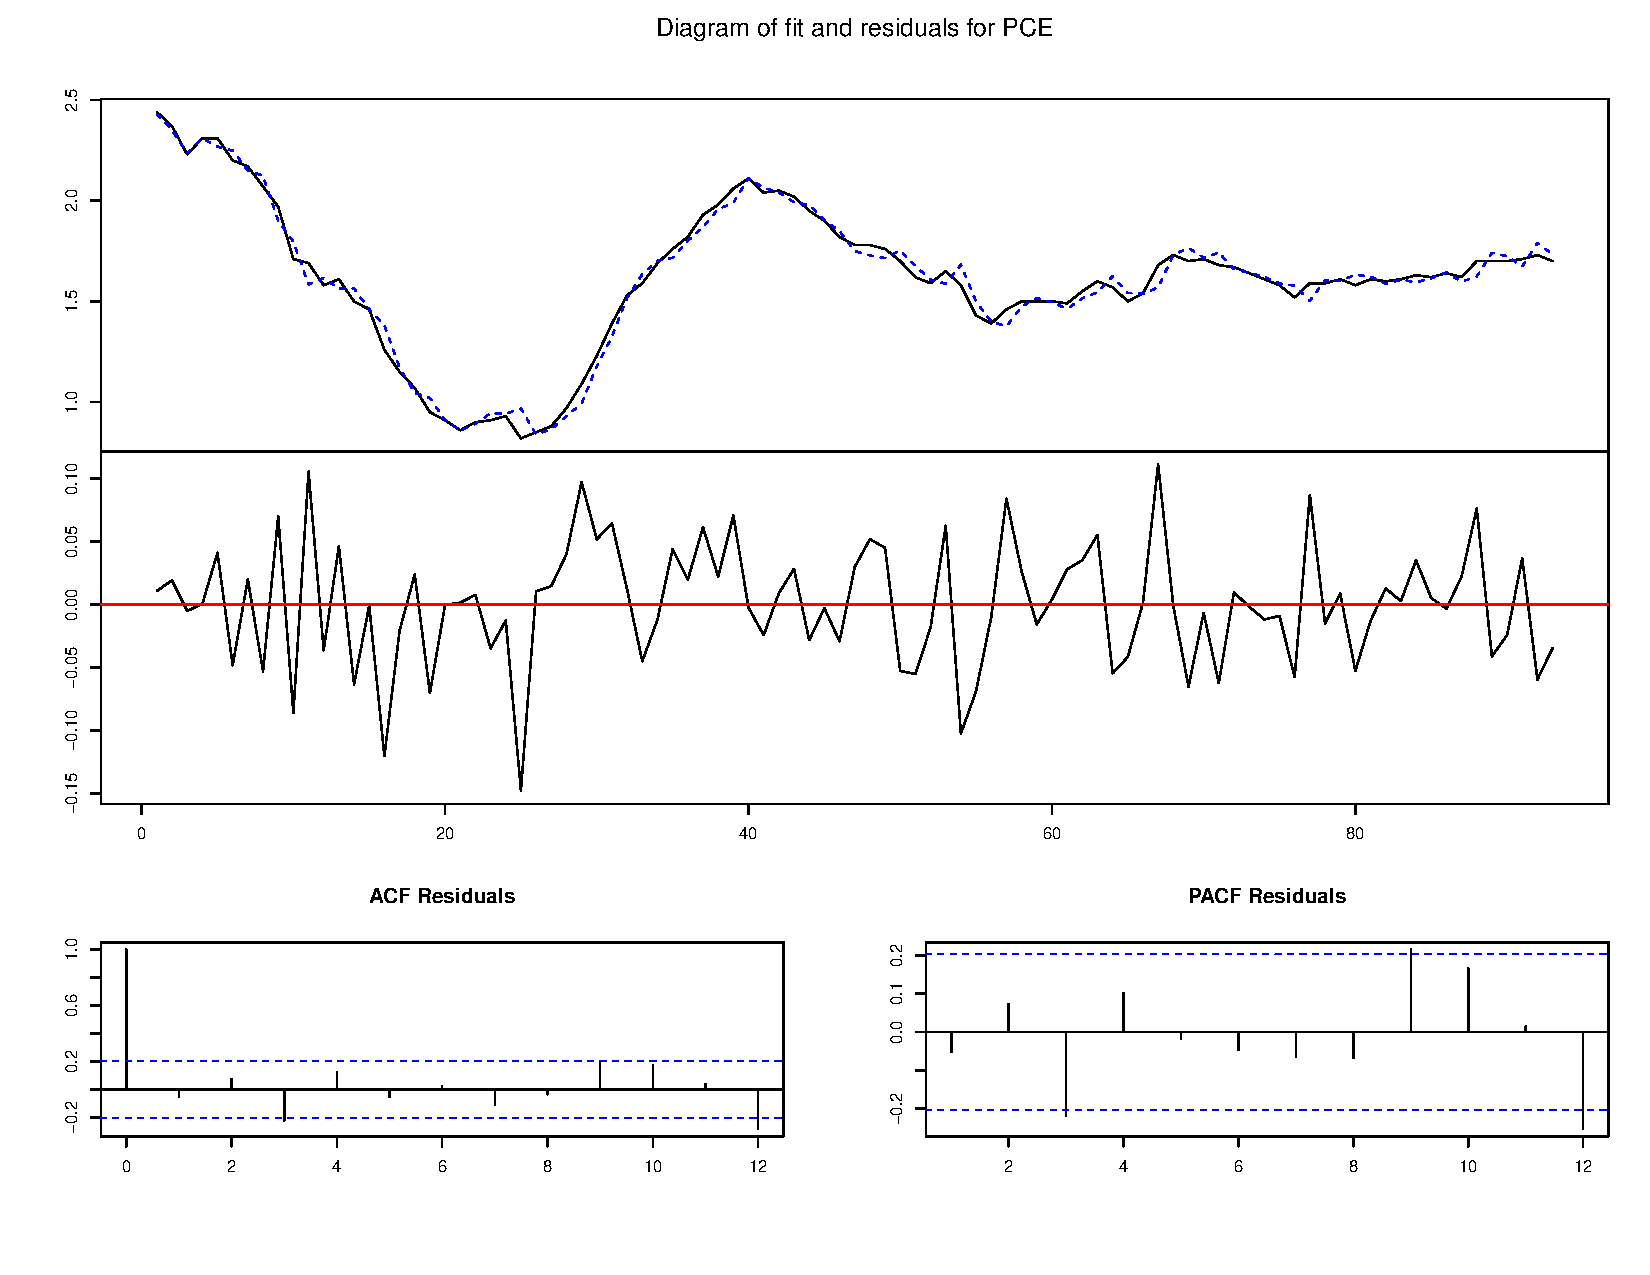
\includegraphics[height=4in]{PCE}
\end{subfigure}
\vspace{-0.75cm}
\begin{flushleft}
\hspace{1cm}\textit{\footnotesize{Źródło: Opracowanie własne.}} \\
\end{flushleft}
\end{figure}

\vspace{-1cm}

\hypertarget{fig101}{}
\begin{figure}[H]
\ContinuedFloat
\centering
\begin{subfigure}{.5\textwidth}
\caption{Stopa bezrobocia}
\hspace{-3cm}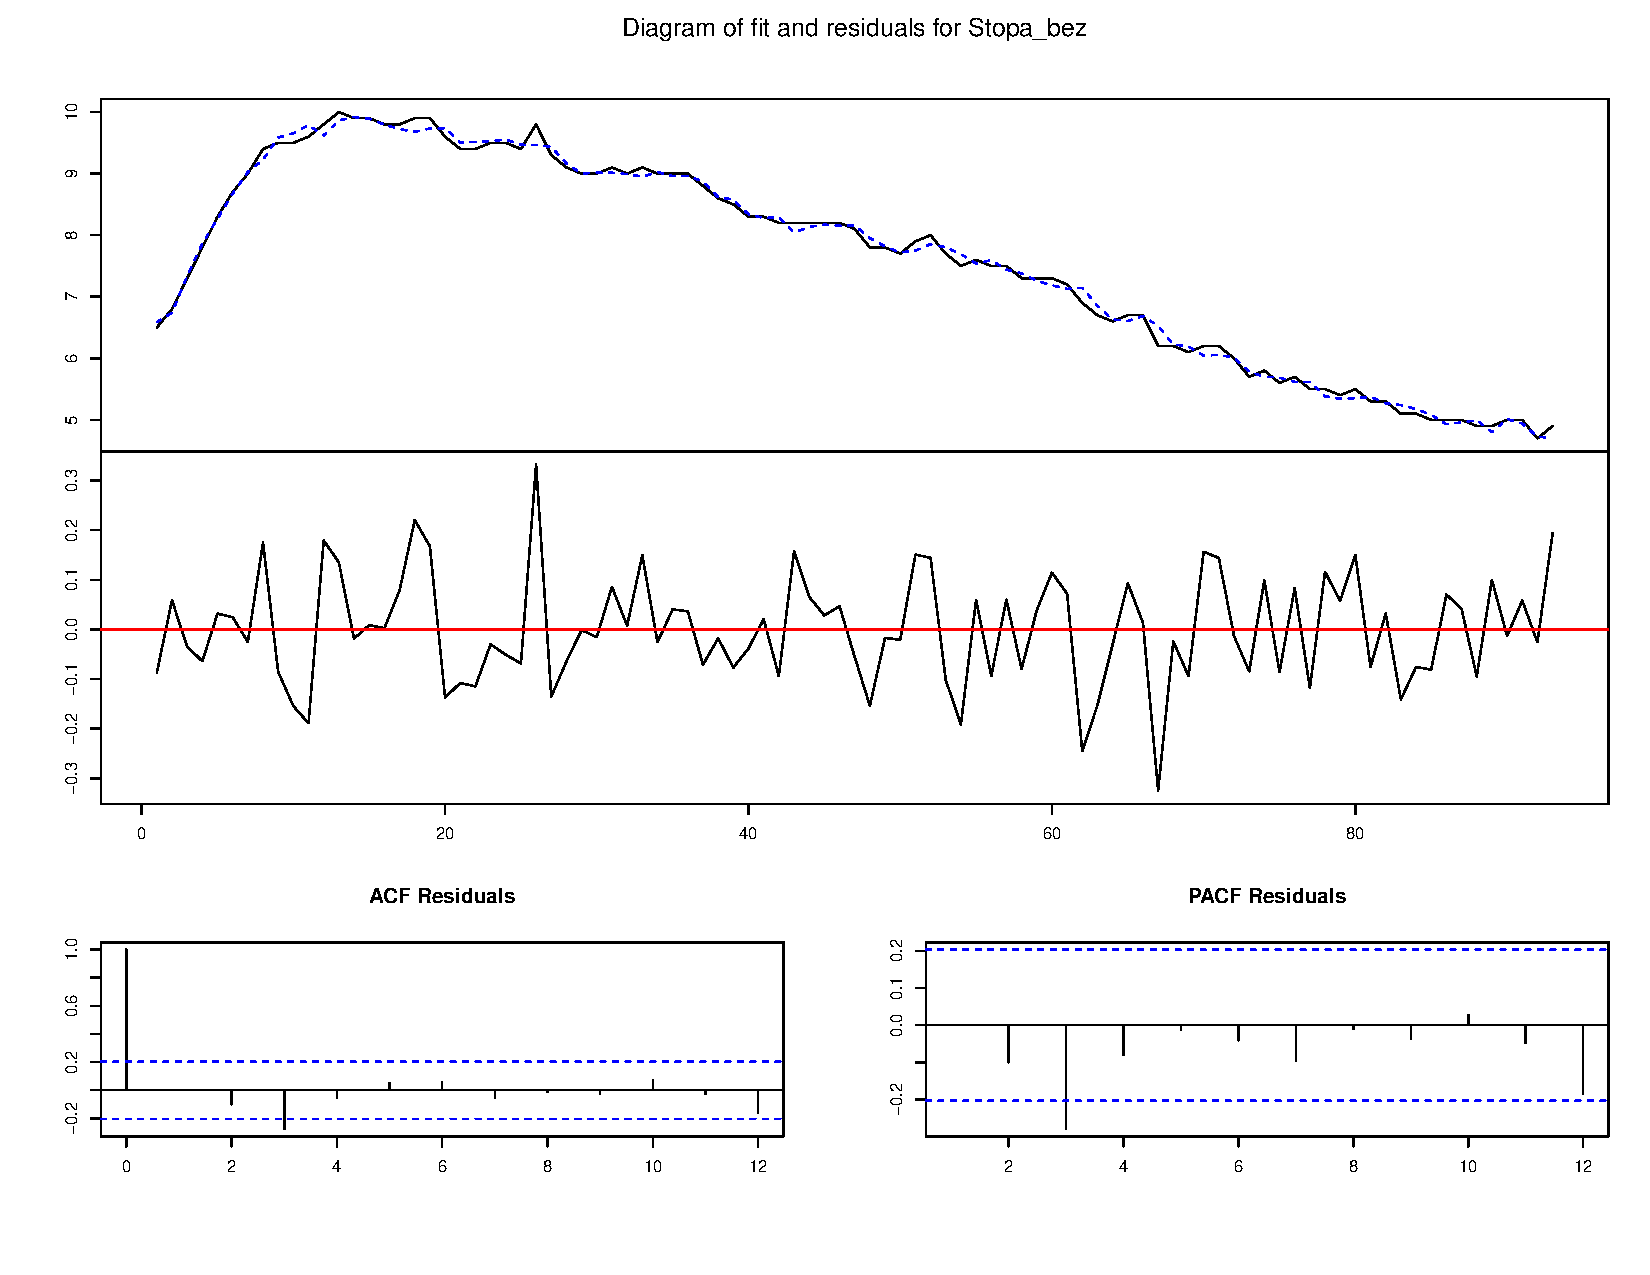
\includegraphics[height=4in]{StopaBez}
\end{subfigure}
\vspace{-0.75cm}
\begin{flushleft}
\hspace{1cm}\textit{\footnotesize{Źródło: Opracowanie własne.}} \\
\end{flushleft}
\end{figure}

\vspace{-1cm}

\hypertarget{fig102}{}
\begin{figure}[H]
\ContinuedFloat
\centering
\begin{subfigure}{.5\textwidth}
\caption{Roczna zmiana PKB realnego}
\hspace{-3cm}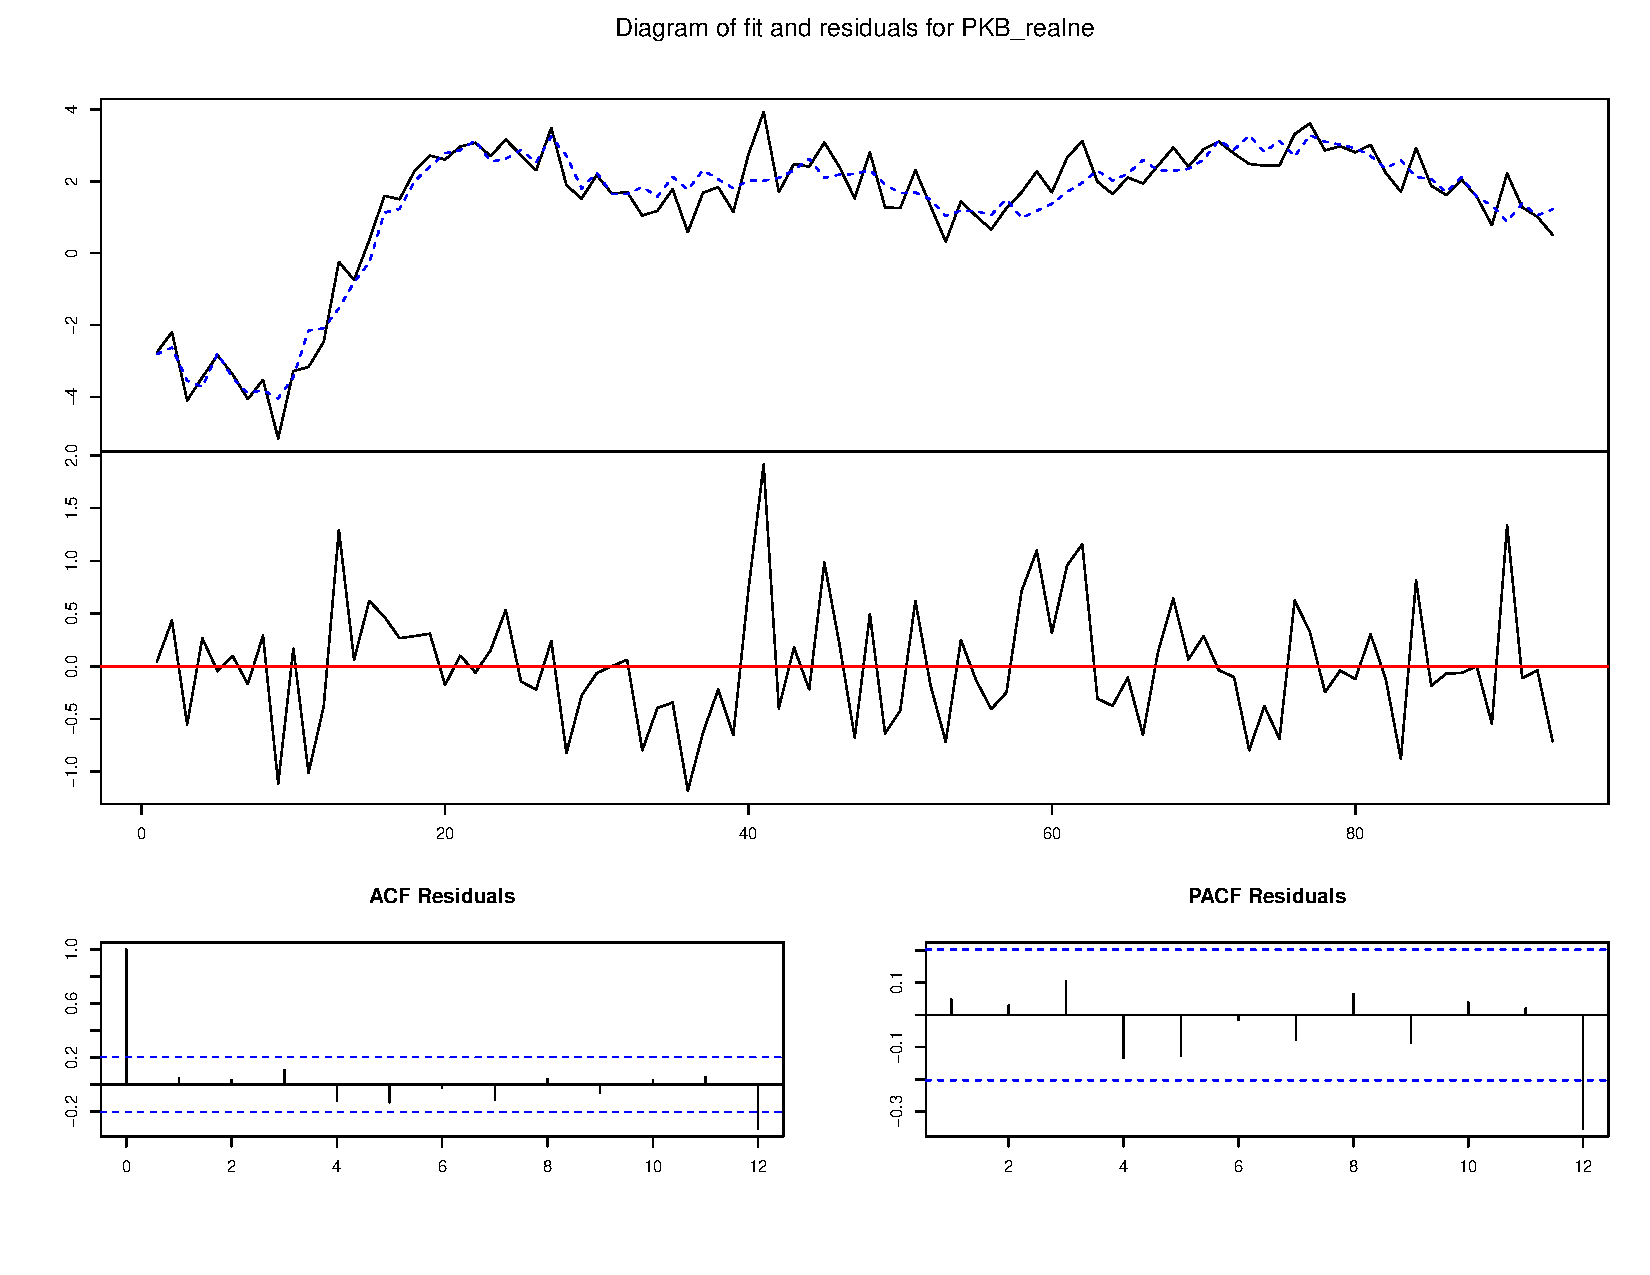
\includegraphics[height=4in]{PKB}
\end{subfigure}
\vspace{-0.75cm}
\begin{flushleft}
\hspace{1cm}\textit{\footnotesize{Źródło: Opracowanie własne.}} \\
\end{flushleft}
\end{figure}

\vspace{-1cm}

\hypertarget{fig103}{}
\begin{figure}[H]
\ContinuedFloat
\centering
\begin{subfigure}{.5\textwidth}
\caption{Indeks S\&P500}
\hspace{-3cm}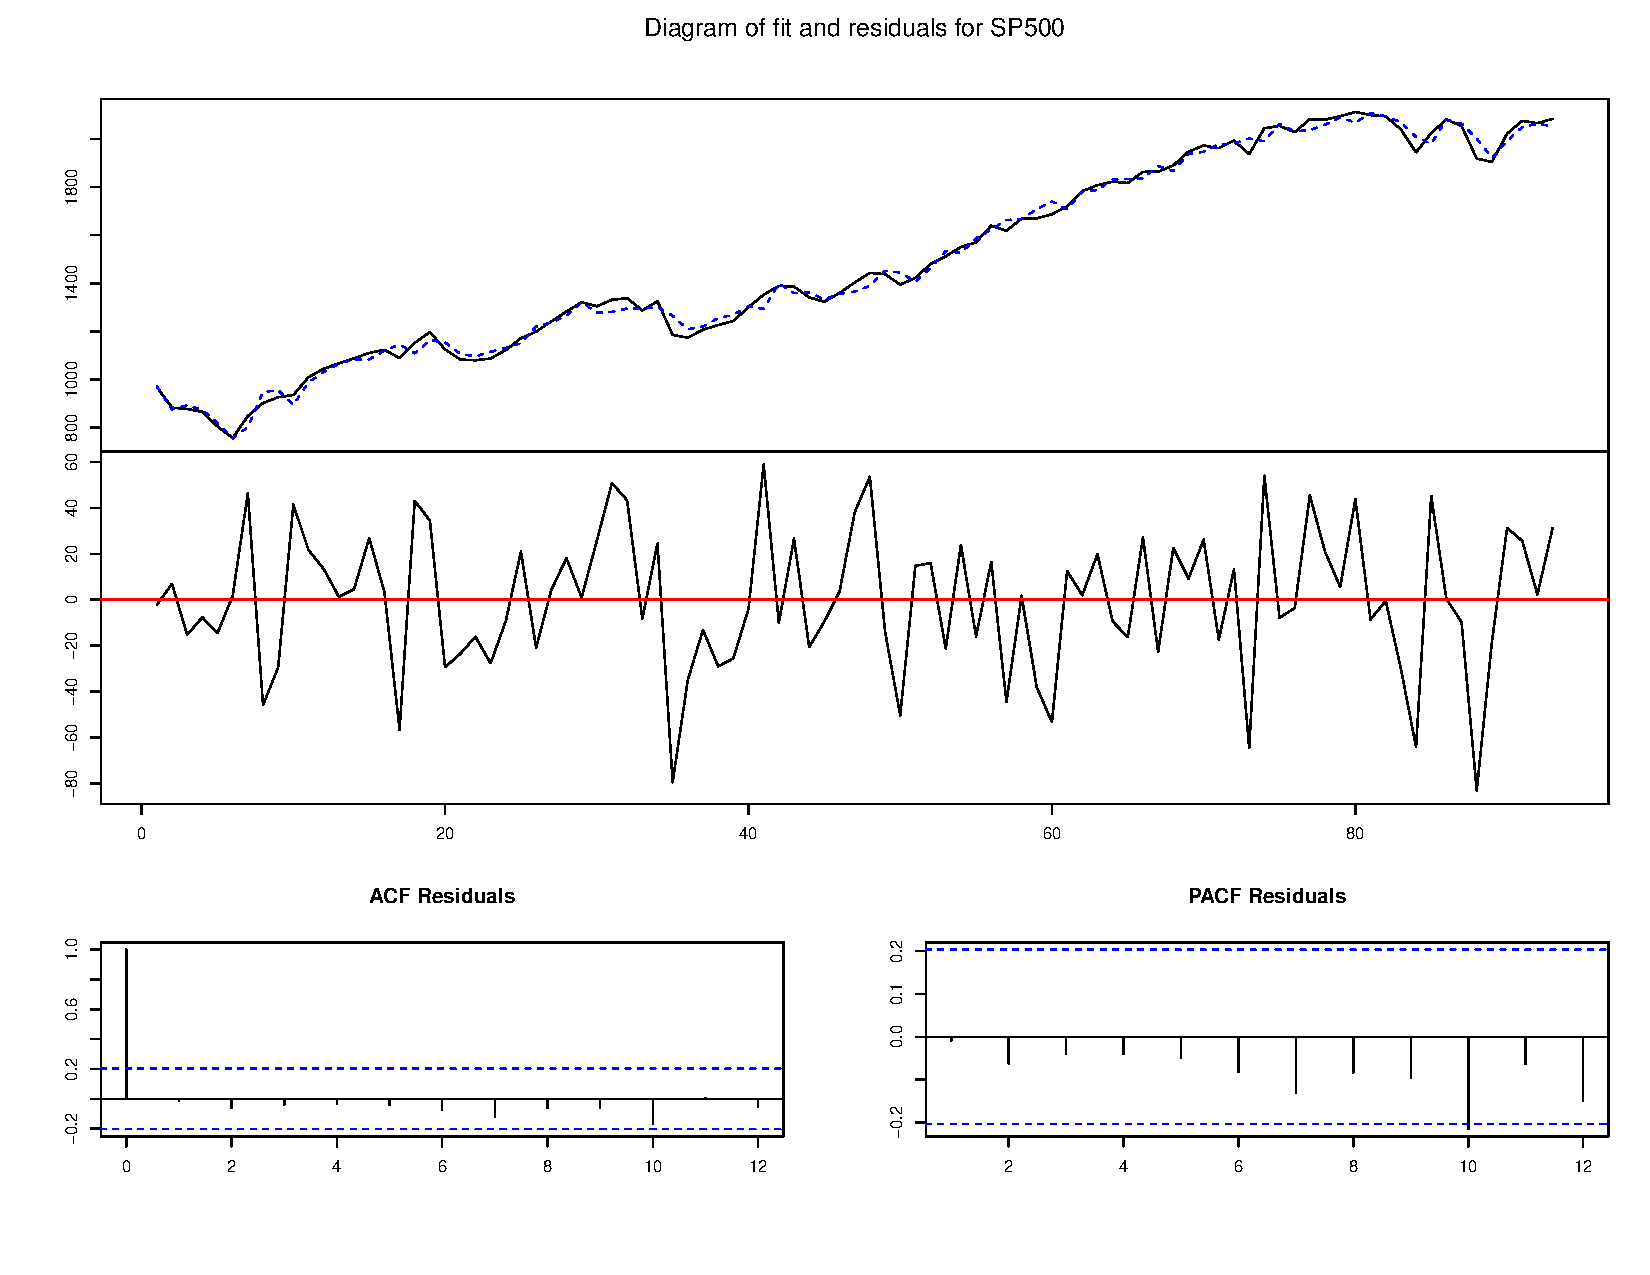
\includegraphics[height=4in]{SP500}
\end{subfigure}
\vspace{-0.75cm}
\begin{flushleft}
\hspace{1cm}\textit{\footnotesize{Źródło: Opracowanie własne.}} \\
\end{flushleft}
\end{figure}

\vspace{-1cm}

\hypertarget{fig104}{}
\begin{figure}[H]
\ContinuedFloat
\centering
\begin{subfigure}{.5\textwidth}
\caption{Rentowność rocznych obligacji skarbowych}
\hspace{-3cm}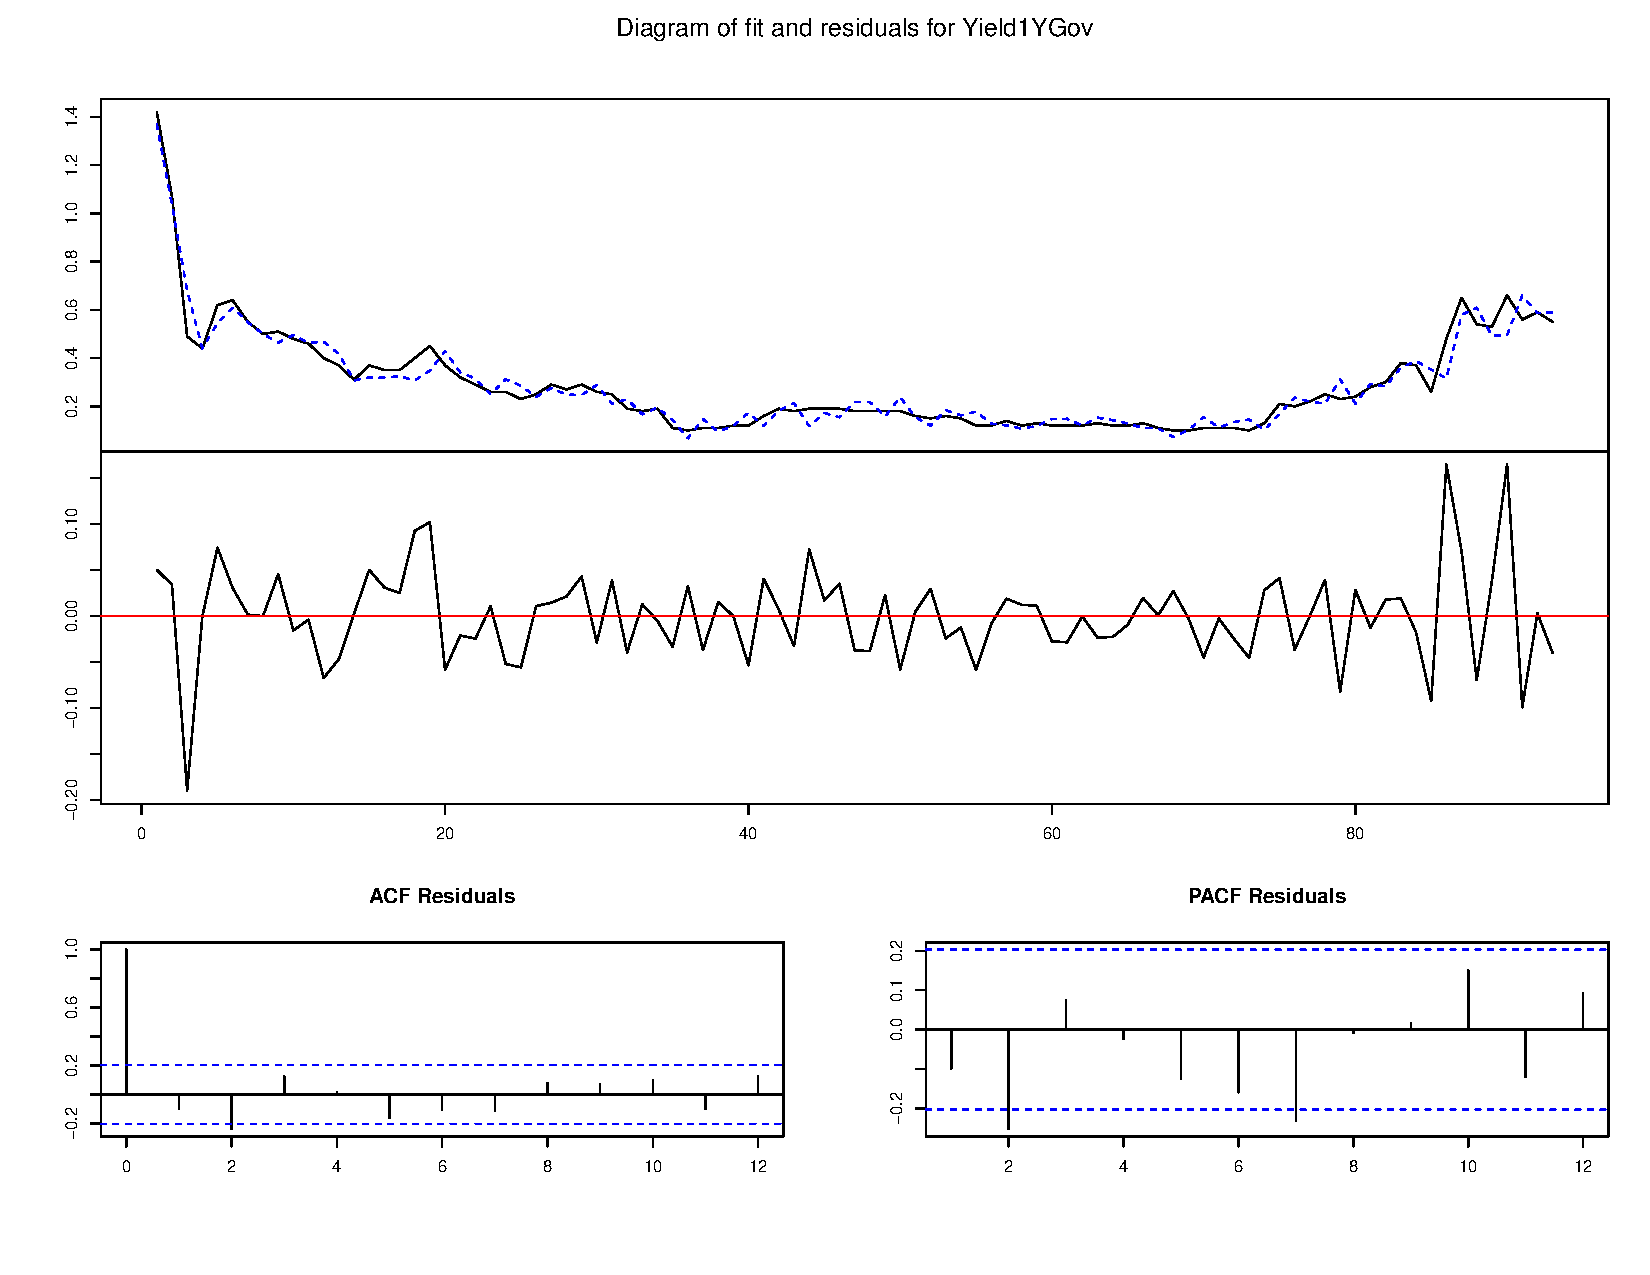
\includegraphics[height=4in]{Yield1}
\end{subfigure}
\vspace{-0.75cm}
\begin{flushleft}
\hspace{1cm}\textit{\footnotesize{Źródło: Opracowanie własne.}} \\
\end{flushleft}
\end{figure}

\vspace{-1cm}

\hypertarget{fig105}{}
\begin{figure}[H]
\ContinuedFloat
\centering
\begin{subfigure}{.5\textwidth}
\caption{Rentowność 10-letnich obligacji skarbowych}
\hspace{-3cm}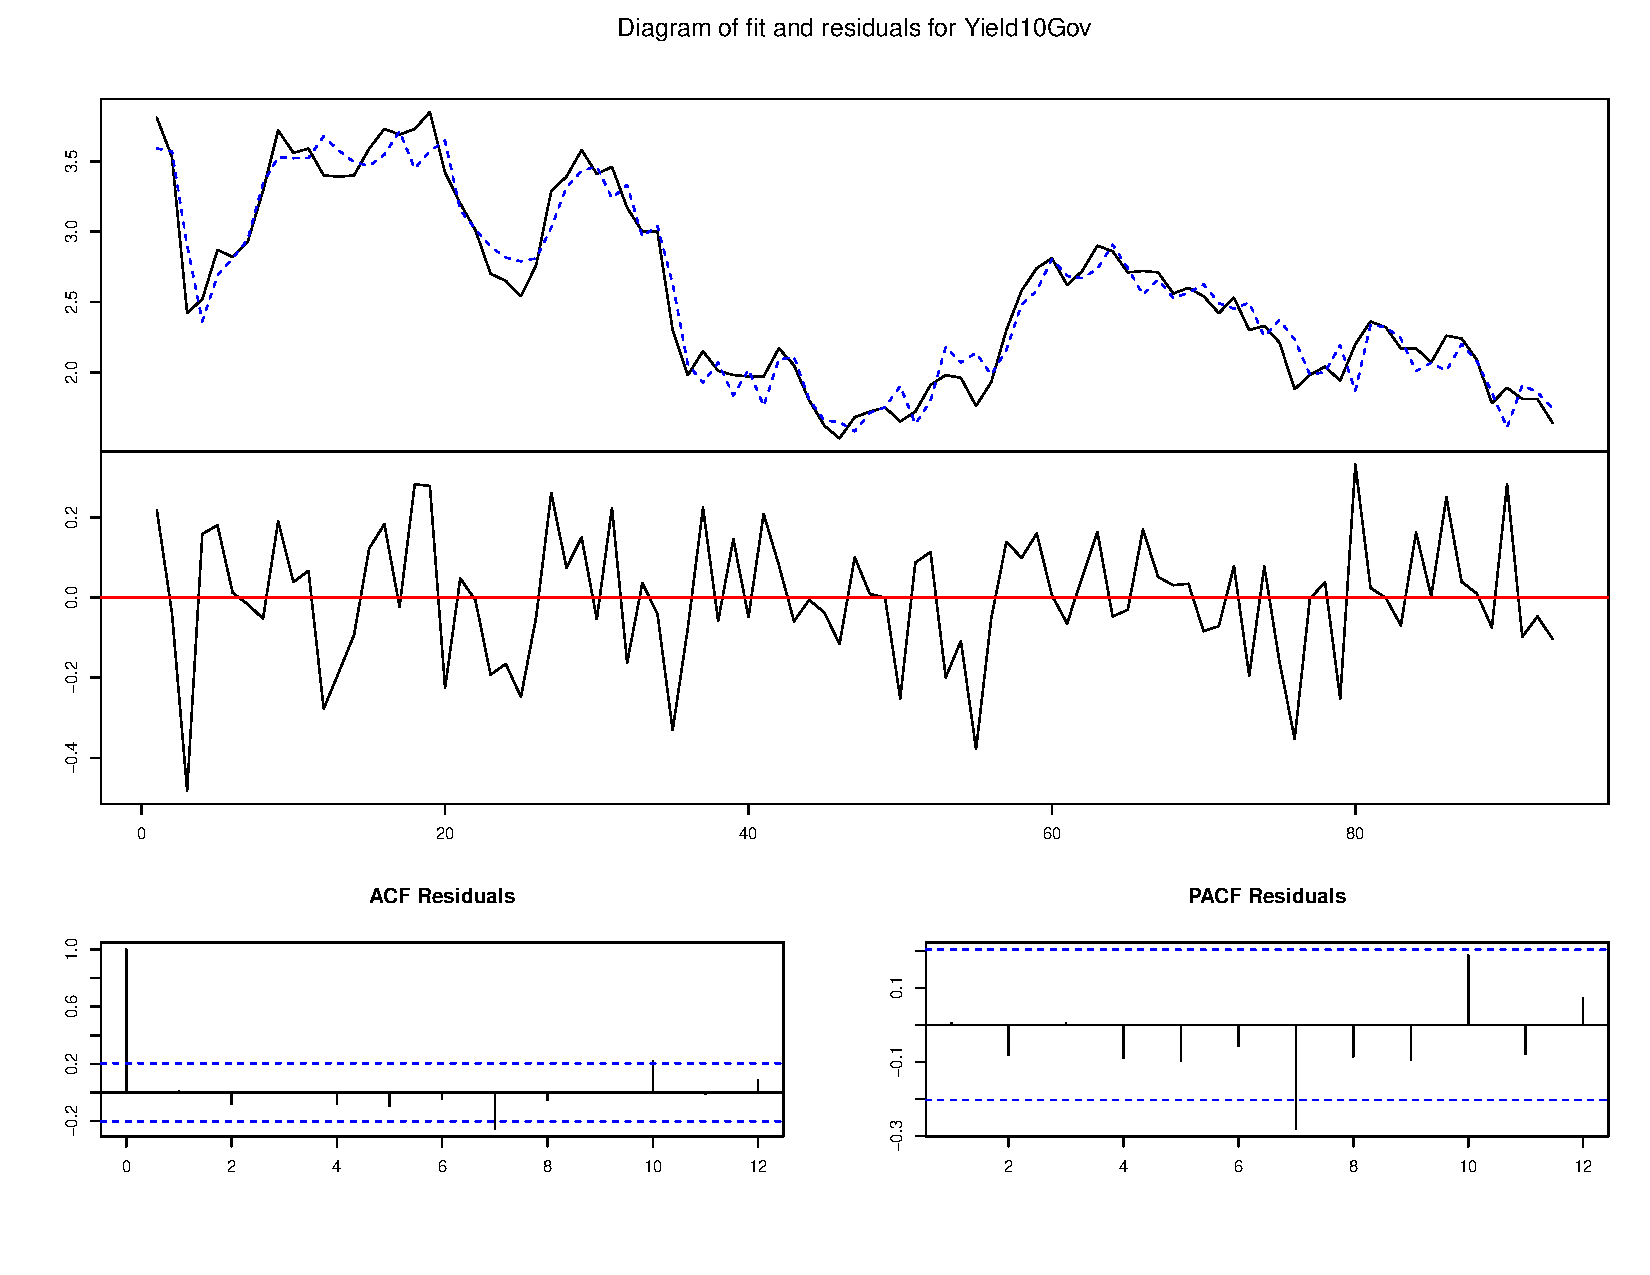
\includegraphics[height=4in]{Yield10}
\end{subfigure}
\vspace{-0.75cm}
\begin{flushleft}
\hspace{1cm}\textit{\footnotesize{Źródło: Opracowanie własne.}} \\
\end{flushleft}
\end{figure}

\vspace{-1cm}

\hypertarget{fig106}{}
\begin{figure}[H]
\ContinuedFloat
\centering
\begin{subfigure}{.5\textwidth}
\caption{Wartość papierów wartościowych FED}
\hspace{-3cm}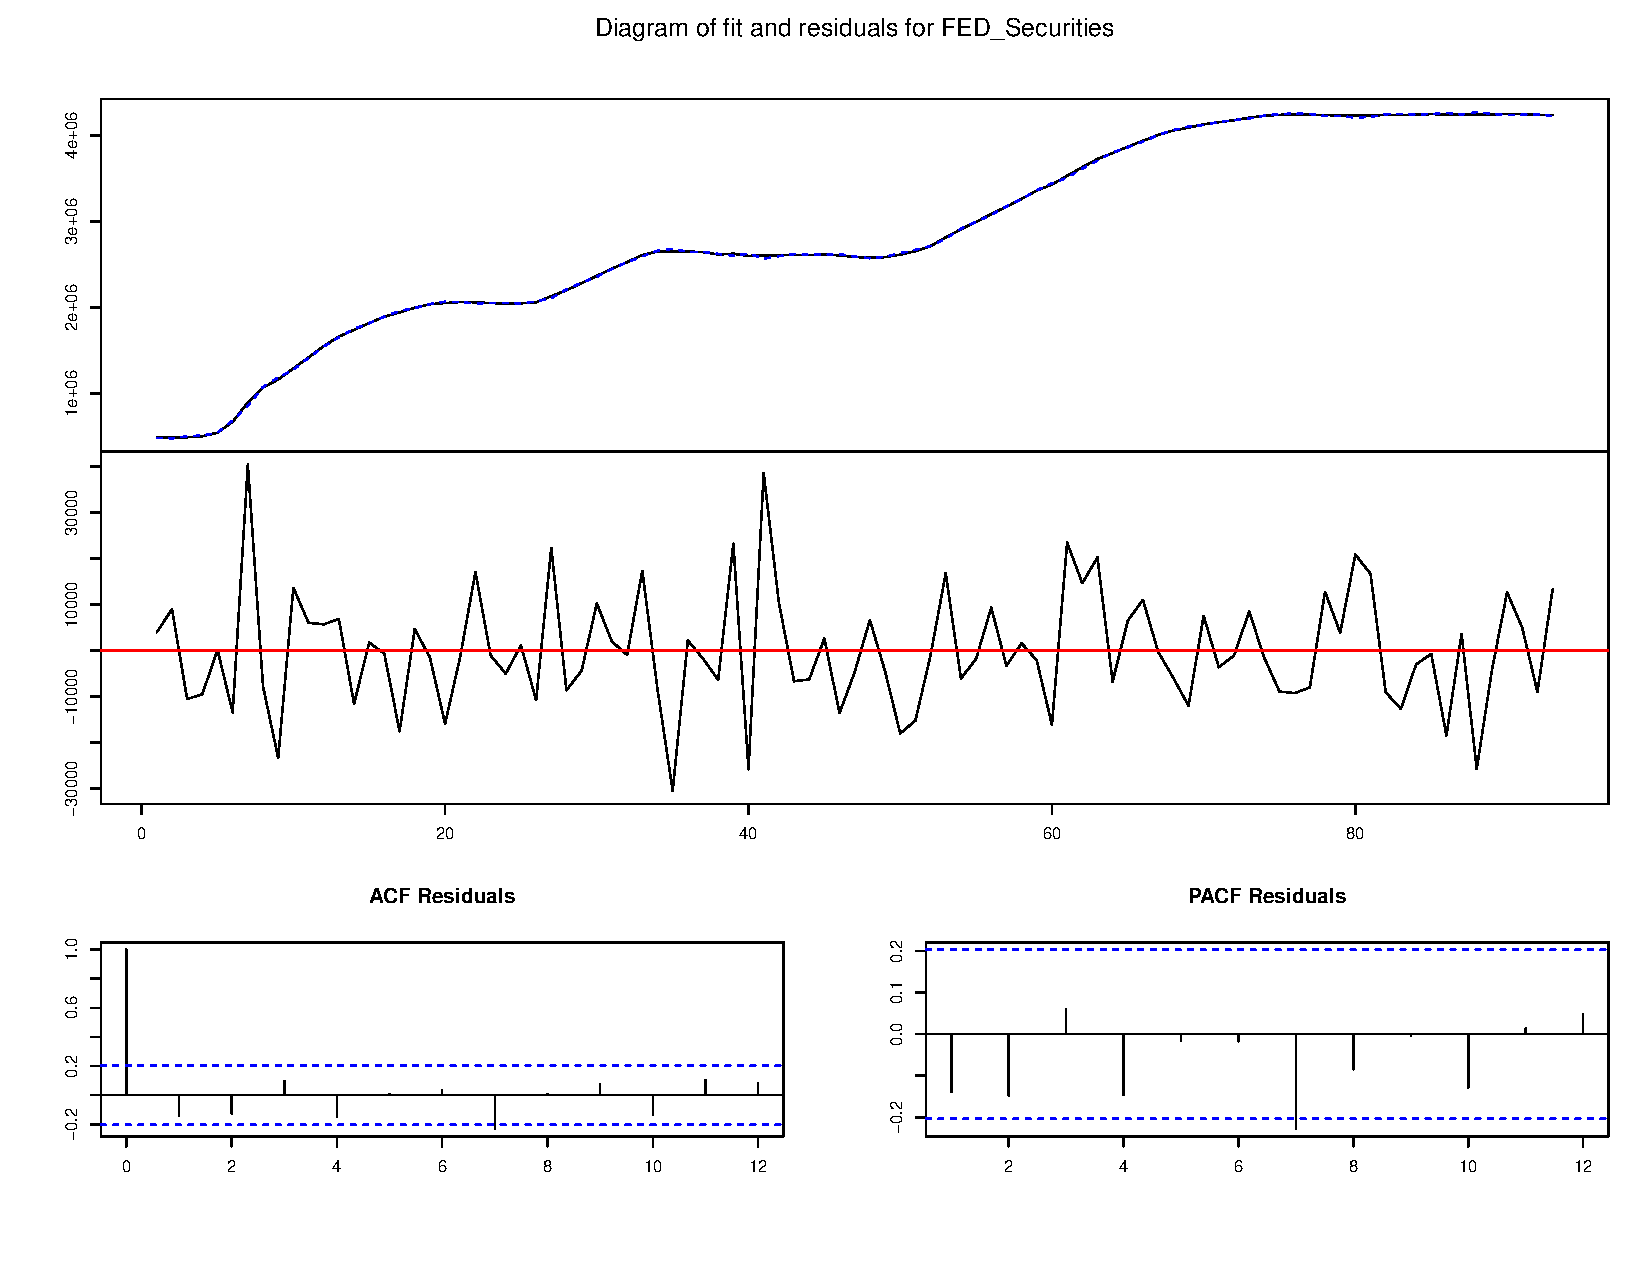
\includegraphics[height=4in]{FED}
\end{subfigure}
\vspace{-0.75cm}
\begin{flushleft}
\hspace{1cm}\textit{\footnotesize{Źródło: Opracowanie własne.}} \\
\end{flushleft}
\end{figure}

\vspace{-1cm}

\hypertarget{fig107}{}
\begin{figure}[H]
\ContinuedFloat
\centering
\begin{subfigure}{.5\textwidth}
\caption{Mediana czasu trwania bezrobocia}
\hspace{-3cm}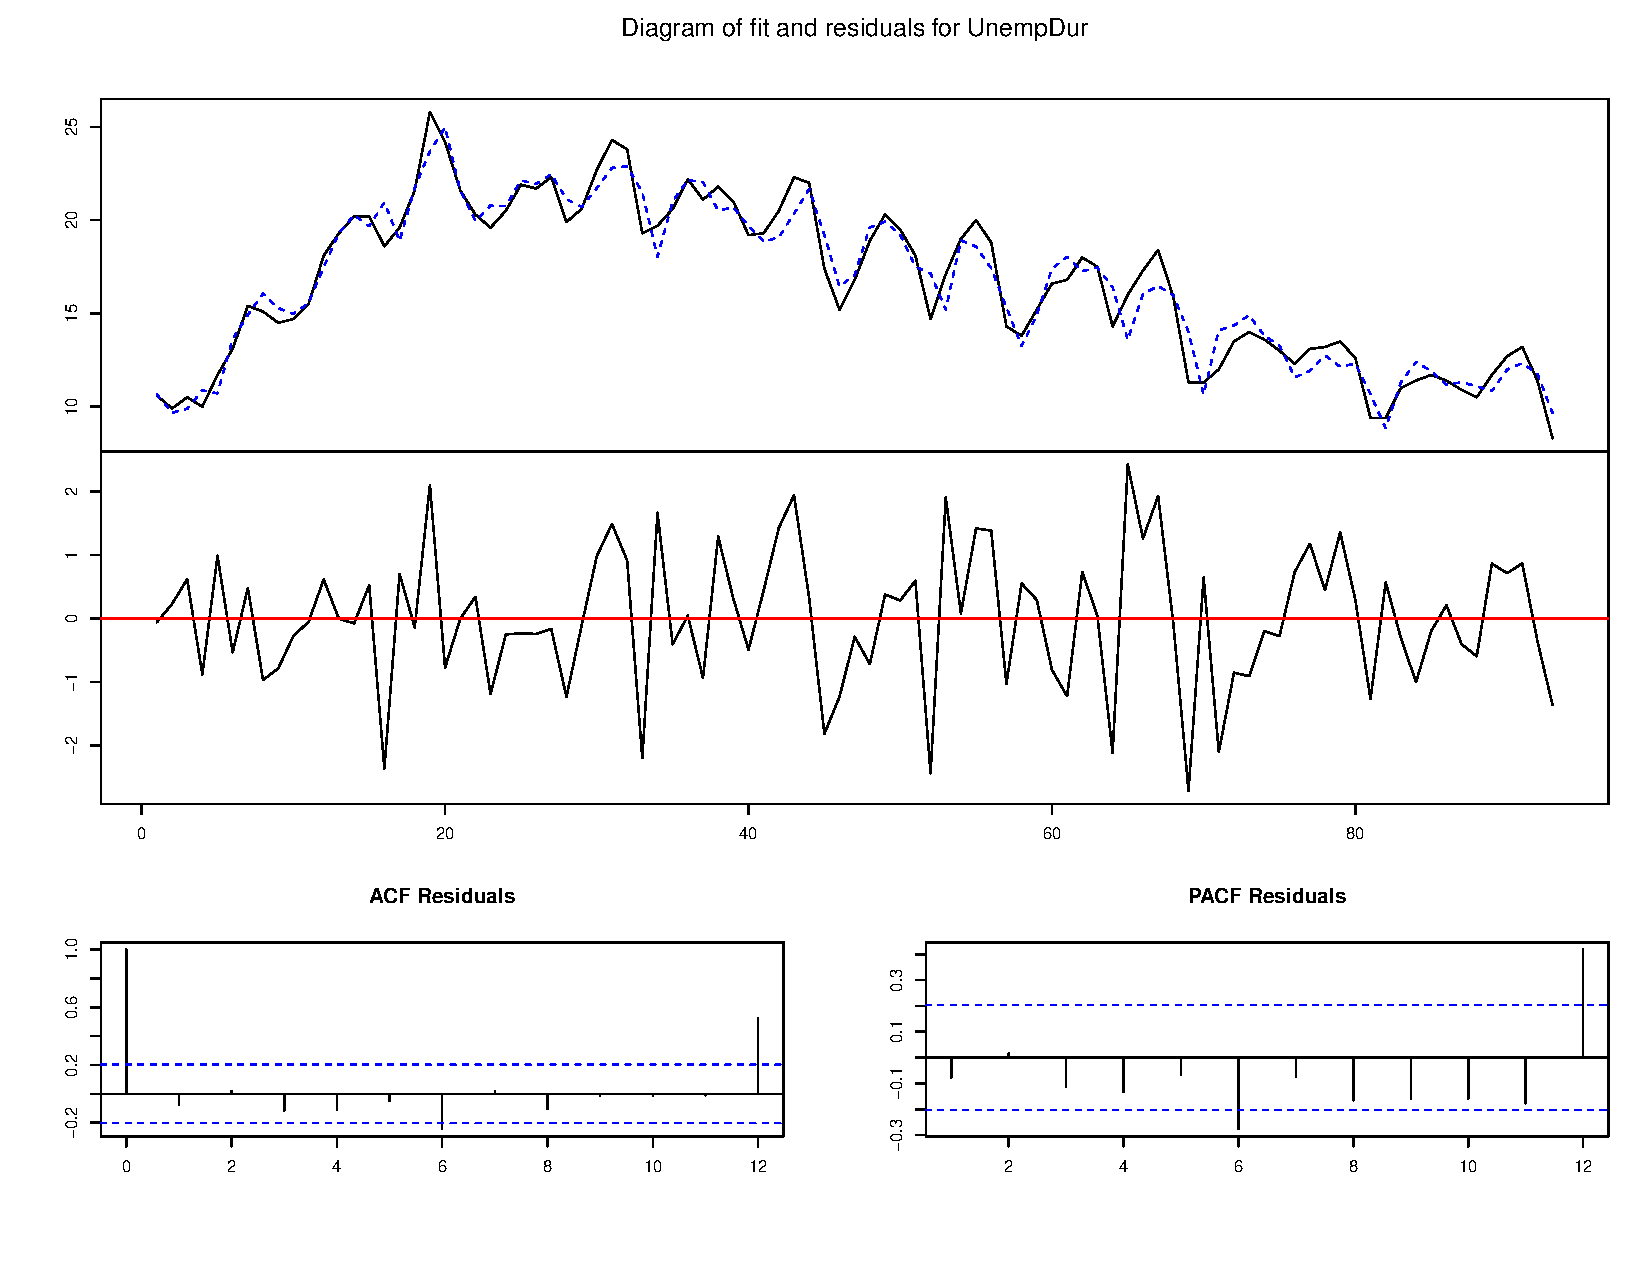
\includegraphics[height=4in]{Unemp}
\end{subfigure}
\vspace{-0.75cm}
\begin{flushleft}
\hspace{1cm}\textit{\footnotesize{Źródło: Opracowanie własne.}} \\
\end{flushleft}
\end{figure}

\vspace{-1cm}

\hypertarget{fig108}{}
\begin{figure}[H]
\ContinuedFloat
\centering
\begin{subfigure}{.5\textwidth}
\caption{Kurs walutowy EUR/USD}
\hspace{-3cm}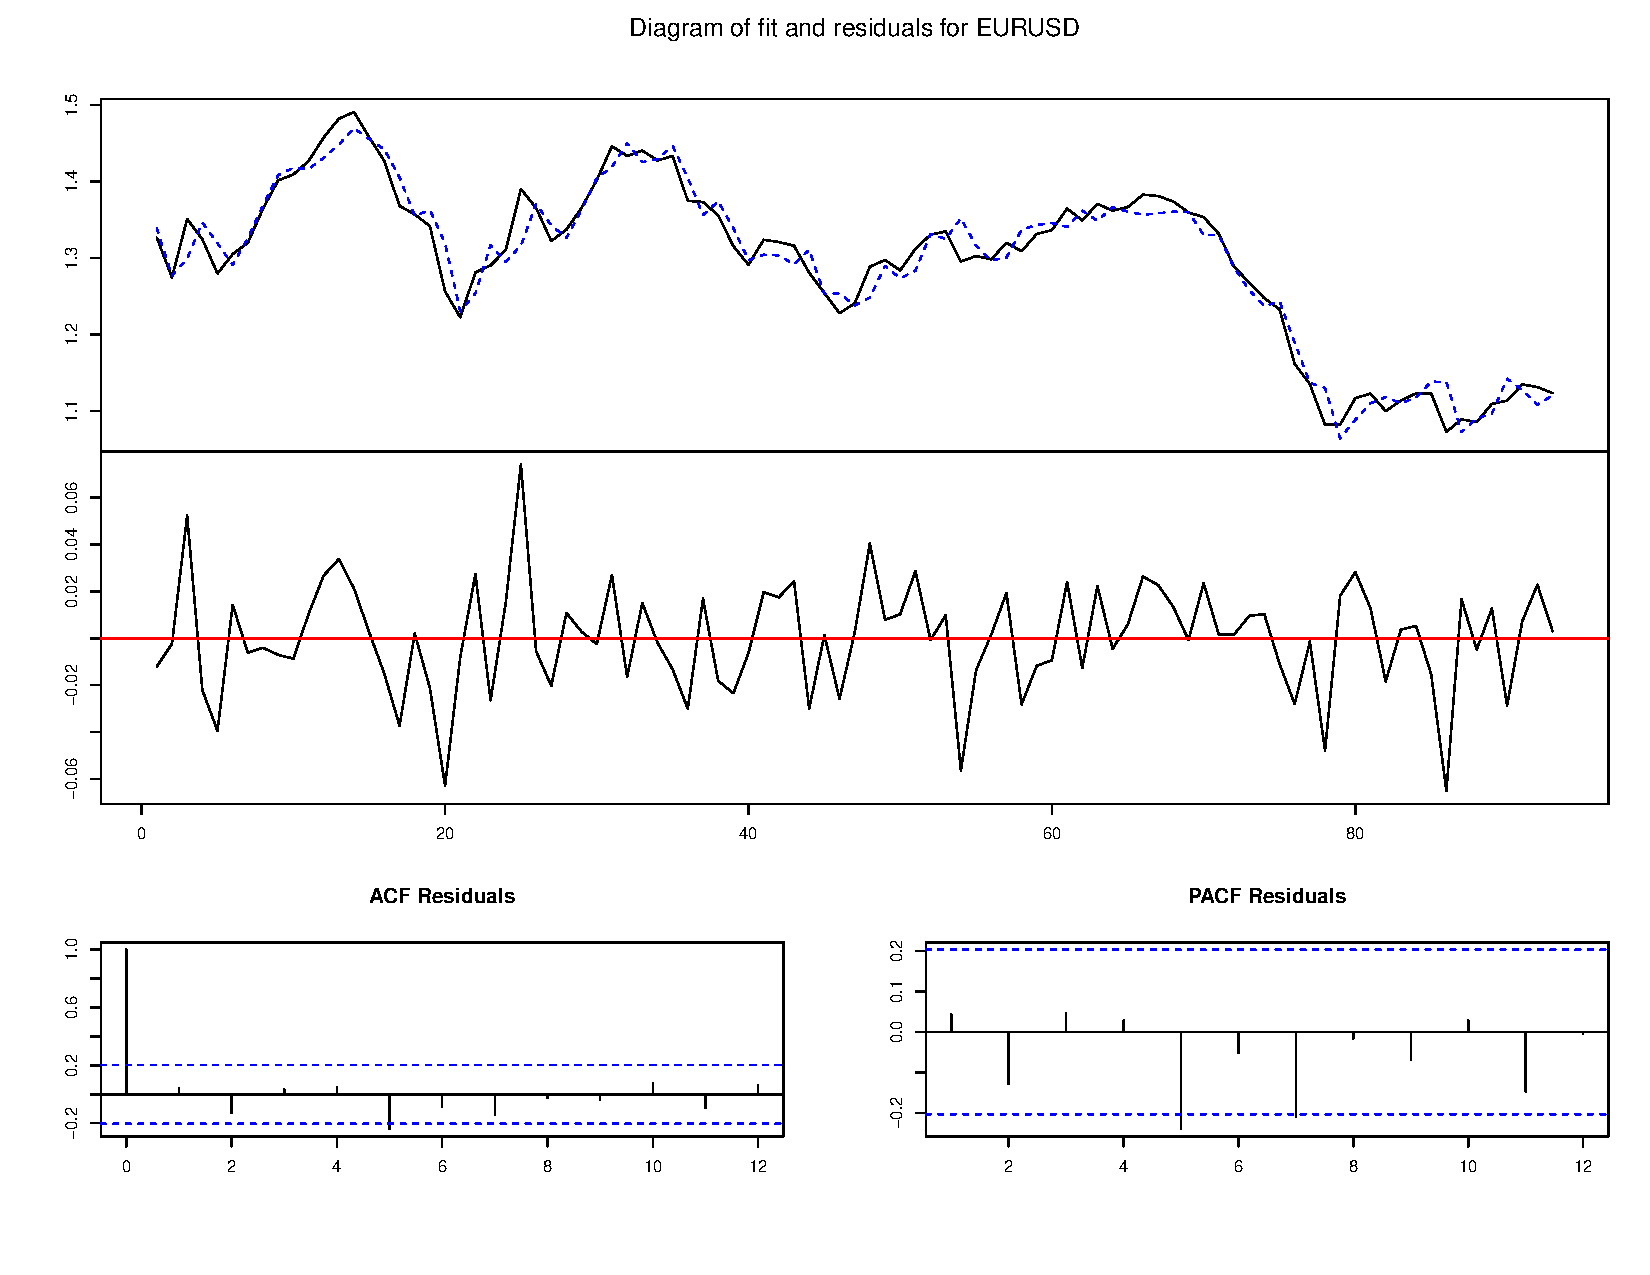
\includegraphics[height=4in]{EURUSD}
\end{subfigure}
\vspace{-0.75cm}
\begin{flushleft}
\hspace{1cm}\textit{\footnotesize{Źródło: Opracowanie własne.}} \\
\end{flushleft}
\end{figure}


%============================================================
\end{document}

%============================================================